\documentclass[a4paper,12pt]{article}

\documentclass[a4paper,12pt]{article}

%%% Работа с русским языком
\usepackage{cmap}					% поиск в PDF
\usepackage{mathtext} 				% русские буквы в формулах
\usepackage[T2A]{fontenc}			% кодировка
\usepackage[utf8]{inputenc}			% кодировка исходного текста
\usepackage[russian,english]{babel}	% локализация и переносы
\usepackage{indentfirst}            % красная строка в первом абзаце
\frenchspacing                      % равные пробелы между словами и предложениями

%%% Дополнительная работа с математикой
\usepackage{amsmath,amsfonts,amssymb,amsthm,mathtools} % пакеты AMS
\usepackage{icomma}                                    % "Умная" запятая

%%% Свои символы и команды
\usepackage{centernot} % центрированное зачеркивание символа
\usepackage{stmaryrd}  % некоторые спецсимволы

\usepackage{ifthen}

\renewcommand{\epsilon}{\ensuremath{\varepsilon}}
\renewcommand{\phi}{\ensuremath{\varphi}}
\renewcommand{\kappa}{\ensuremath{\varkappa}}
\renewcommand{\le}{\ensuremath{\leqslant}}
\renewcommand{\leq}{\ensuremath{\leqslant}}
\renewcommand{\ge}{\ensuremath{\geqslant}}
\renewcommand{\geq}{\ensuremath{\geqslant}}
\renewcommand{\emptyset}{\ensuremath{\varnothing}}

\DeclareMathOperator{\sgn}{sgn}
\DeclareMathOperator{\ke}{Ker}
\DeclareMathOperator{\im}{Im}
\DeclareMathOperator{\re}{Re}

\newcommand{\N}{\mathbb{N}}
\newcommand{\Z}{\mathbb{Z}}
\newcommand{\Q}{\mathbb{Q}}
\newcommand{\R}{\mathbb{R}}
\newcommand{\Cm}{\mathbb{C}}
\newcommand{\F}{\mathbb{F}}
\newcommand{\id}{\mathrm{id}}

\newcommand{\imp}[2]{
	(#1\,\,$\ra$\,\,#2)\,\,
}
\newcommand{\System}[1]{
	\left\{\begin{aligned}#1\end{aligned}\right.
}
\newcommand{\Root}[2]{
	\left\{\!\sqrt[#1]{#2}\right\}
}

\renewcommand\labelitemi{$\triangleright$}

\let\bs\backslash
\let\Lra\Leftrightarrow
\let\lra\leftrightarrow
\let\Ra\Rightarrow
\let\ra\rightarrow
\let\La\Leftarrow
\let\la\leftarrow
\let\emb\hookrightarrow

%%% Перенос знаков в формулах (по Львовскому)
\newcommand{\hm}[1]{#1\nobreak\discretionary{}{\hbox{$\mathsurround=0pt #1$}}{}}

%%% Работа с картинками
\usepackage{graphicx}    % Для вставки рисунков
\setlength\fboxsep{3pt}  % Отступ рамки \fbox{} от рисунка
\setlength\fboxrule{1pt} % Толщина линий рамки \fbox{}
\usepackage{wrapfig}     % Обтекание рисунков текстом

%%% Работа с таблицами
\usepackage{array,tabularx,tabulary,booktabs} % Дополнительная работа с таблицами
\usepackage{longtable}                        % Длинные таблицы
\usepackage{multirow}                         % Слияние строк в таблице

%%% Теоремы
\theoremstyle{plain}
\newtheorem{theorem}[equation]{Theorem}
\newtheorem{lemma}[equation]{Lemma}
\newtheorem{proposition}[equation]{Proposition}
\newtheorem*{exercise}{Exercise}
\newtheorem*{problem}{Problem}

\theoremstyle{definition}
\newtheorem{definition}[equation]{Definition}
\newtheorem*{corollary}{Corollary}
\newtheorem*{note}{Note}
\newtheorem*{reminder}{Reminder}
\newtheorem*{example}{Example}

\theoremstyle{remark}
\newtheorem*{solution}{Solution}

%%% Оформление страницы
\usepackage{extsizes}     % Возможность сделать 14-й шрифт
\usepackage{geometry}     % Простой способ задавать поля
\usepackage{setspace}     % Интерлиньяж
\usepackage{enumitem}     % Настройка окружений itemize и enumerate
\setlist{leftmargin=25pt} % Отступы в itemize и enumerate

\geometry{top=25mm}    % Поля сверху страницы
\geometry{bottom=30mm} % Поля снизу страницы
\geometry{left=20mm}   % Поля слева страницы
\geometry{right=20mm}  % Поля справа страницы

\setlength\parindent{0pt}         % Устанавливает длину красной строки 0pt
\linespread{1.3}                  % Коэффициент межстрочного интервала
%\setlength{\parskip}{0.5em}      % Вертикальный интервал между абзацами
%\setcounter{secnumdepth}{0}      % Отключение нумерации разделов
%\setcounter{section}{-1}         % Нумерация секций с нуля
\usepackage{multicol}			  % Для текста в нескольких колонках
\usepackage{soulutf8}             % Модификаторы начертания

%%% Содержаниие
\usepackage{tocloft}
\tocloftpagestyle{main}
%\setlength{\cftsecnumwidth}{2.3em}
%\renewcommand{\cftsecdotsep}{1}
%\renewcommand{\cftsecpresnum}{\hfill}
%\renewcommand{\cftsecaftersnum}{\quad}

%%% Шаблонная информация для титульного листа
\newcommand{\CourseName}{Introduction to Calculus}
\newcommand{\FullCourseNameFirstPart}{\so{INTRODUCTION TO CALCULUS}}
\newcommand{\SemesterNumber}{I}
\newcommand{\LecturerInitials}{Nikolay Gusev}
\newcommand{\CourseDate}{fall 2022}
\newcommand{\AuthorInitials}{Danil Klishch}
\newcommand{\VKLink}{https://vk.com/dan.klishch}
\newcommand{\GithubLink}{https://github.com/daniild71r/lectures_tex_club}

%%% Колонтитулы
\usepackage{titleps}
\newpagestyle{main}{
	\setheadrule{0.4pt}
	\sethead{\CourseName}{}{\hyperlink{intro}{\;Back to table of contents}}
	\setfootrule{0.4pt}                       
	\setfoot{MIPT, \CourseDate}{}{\thepage} 
}
\pagestyle{main}

%%% Нумерация уравнений
\makeatletter
\def\eqref{\@ifstar\@eqref\@@eqref}
\def\@eqref#1{\textup{\tagform@{\ref*{#1}}}}
\def\@@eqref#1{\textup{\tagform@{\ref{#1}}}}
\makeatother                      % \eqref* без гиперссылки
\numberwithin{equation}{subsection}  % Нумерация вида (номер_секции).(номер_уравнения)
\mathtoolsset{showonlyrefs=false} % Номера только у формул с \eqref{} в тексте.

%%% Гиперссылки
\usepackage{hyperref}
\usepackage[usenames,dvipsnames,svgnames,table,rgb]{xcolor}
\hypersetup{
	unicode=true,            % русские буквы в раздела PDF
	colorlinks=true,       	 % Цветные ссылки вместо ссылок в рамках
	linkcolor=black!15!blue, % Внутренние ссылки
	citecolor=green,         % Ссылки на библиографию
	filecolor=magenta,       % Ссылки на файлы
	urlcolor=NavyBlue,       % Ссылки на URL
}

%%% Графика
\usepackage{tikz}        % Графический пакет tikz
\usepackage{tikz-cd}     % Коммутативные диаграммы
\usepackage{tkz-euclide} % Геометрия
\usepackage{stackengine} % Многострочные тексты в картинках
\usetikzlibrary{angles, babel, quotes}

%%% Мои кастомные команды
\newcommand{\df}[2]{\begin{definition}\textit{#1} -- #2\end{definition}}

\newcommand{\abs}[1]{\left\lvert #1 \right\rvert}
\newcommand{\grad}{\mathrm{grad}\:}
\newcommand{\dlta}{\text{d}}
\newcommand{\thus}{\;\Rightarrow\;}
\newcommand{\isconst}{=\text{const}}

\newcommand{\defeq}{\vcentcolon=}
\newcommand{\defev}{\stackrel{\Delta}{\Longleftrightarrow}}
\newcommand{\deriv}[3][1]{%
	\ifthenelse{#1>1}{%
		\frac{\dlta^{#1} {#2}}{\dlta {#3}^{#1}}
	}{%
		\frac{\dlta {#2}}{\dlta {#3}}
	}%
}
\newcommand{\vc}[3]{
	\ensuremath{\begin{pmatrix} #1 \\ #2 \\ #3 \end{pmatrix}}
}
\newcommand{\vb}[2]{
	\ensuremath{\begin{pmatrix} #1 \\ #2 \end{pmatrix}}
}
\newcommand{\fnis}[1]{#1{:}\;}
\newcommand{\RR}{\mathbb{R}}
\newcommand{\NN}{\mathbb{N}}
\newcommand{\sconstr}{\;\vert\;}
\newcommand{\diag}{{\rm diag}}

\newcommand{\floor}[1]{\left\lfloor#1\right\rfloor}
\newcommand{\ceil}[1]{\left\lceil#1\right\rceil}


%%% Всю шаблонную информацию можно менять тут
\newcommand{\FullCourseNameFirstPart}{\so{ТЕОРИЯ~ФУНКЦИЙ}}
\newcommand{\FullCourseNameSecondPart}{\so{КОМПЛЕКСНОГО~ПЕРЕМЕННОГО}}
\newcommand{\SchoolName}{ФПМИ}
\newcommand{\TrackName}{ПМФ}
\newcommand{\SemesterNumber}{V}
\newcommand{\LecturerInitials}{Половинкин Евгений Сергеевич}
\newcommand{\AutherInitials}{Маланчук София}
\newcommand{\VKLink}{https://vk.com/smalanchuk0}
\newcommand{\OverleafLink}{https://www.overleaf.com/read/vgjwvzdrzvqc}
\newcommand{\GithubLink}{https://github.com/MIPT-Group/Lectures_Tex_Club/}
\newcommand{\CourseName}{ТФКП} %  Используется в преамбуле для создания названия предмета в верхнем контитуле   
\newcommand{\CourseDate}{Осень 2020}           %  Используется в преамбуле для создания даты в нижнем контитуле

%\includeonly{lectures/lect05,lectures/lect06}  % Чтобы скомпилировать только часть лекций

\begin{document}
    \begin{titlepage}
	\clearpage\thispagestyle{empty}
	\centering
	
	\textit{Федеральное государственное автономное учреждение \\
		высшего образования}
	\vspace{0.5ex}
	
	\textbf{Московский физико-технический институт
    \\
    (национальный исследовательский университет)
    \\
     КЛУБ ТЕХА ЛЕКЦИЙ}
	\vspace{20ex}
	
	\rule{\linewidth}{0.5mm}
	{\textbf{\FullCourseNameFirstPart}}
	\\
	{\textbf{\FullCourseNameSecondPart}}
	\rule{\linewidth}{0.5mm}
	
	\SemesterNumber\ СЕМЕСТР
	\\
	Физтех-школа: \textit{\SchoolName}
	\\
	Направление: \textit{\TrackName}
	\\
	Лектор: \textit{\LecturerInitials}
	\vspace{1ex}
	
	\begin{figure}[!ht]
		\centering
		\includegraphics[width=0.6\textwidth]{logo_LTC}
	\end{figure}
\begin{flushright}
	\noindent
	Автор(ы): \href{\VKLink}{\textit{\AutherInitials}}
	\\
	\href{\OverleafLink}{\textit{Проект на overleaf}}
	\\
	\href{\GithubLink}{\textit{Проект на github}} 
\end{flushright}
	
	\vfill
	Долгопрудный, \CourseDate\ год.
	\pagebreak
	
\end{titlepage}
    \hypertarget{intro}{}
    \tableofcontents
    \newpage
    \begin{flushright}
    \textit{Лекция 1 (от 07.09)}
\end{flushright}
\section{$\S 1.$ Комплексные числа}
\Def
Пусть $z = \left( x;y \right) \in \RR^2$. Пусть определены операции:
\begin{enumerate}
    \item \textbf{Сложение:} $z_1 + z_2 = \left( x_1+x_2; y_1+y_2 \right)$
    \item \textbf{Умножение на действительное число:} $\lambda z = \left(\lambda
        x, \lambda y \right)$
    \item \textbf{Расстояние:} $\rho(z_1, z_2) = \left| \left| z_1 - z_2 \right|
    \right| = \sqrt{\left( x_1 - x_2 \right)^2 + (y_1 - y_2)^2}$
\end{enumerate}
Добавим операцию
умножения друг на друга:
\begin{align*}
  & z_1 \cdot z_2 = \left( x_1 \cdot x_2 - y_1 \cdot y_2; x_1 \cdot y_2 + x_2 \cdot y_1 \right)
\end{align*}
Будем называть это \textbf{комплексными числами} $\CC$.
\\
Пусть $1 \sim (1; 0)$~--- \textbf{единица}, $i \sim (0;1)$~--- \textbf{мнимая
  единица}.
\\
Тогда $z = 1 \cdot x + i \cdot y \Leftrightarrow z = x + iy$~---
\textbf{алгебраическая запись}.
\\
Назовем $x = \Real z$ \textbf{действительной частью}, $y =
\Img z$~--- \textbf{мнимой}.
\\
\textbf{Сопряженным} к $z = x+iy$ называем $\bar{z} = x-iy$,
\textbf{модулем}~--- выражение $\left| z \right| = \sqrt{x^2+y^2}$. Легко
видеть, что $z\bar{z} = \left| z \right|^2$, полагая $i^2 = -1$.
\\
Можно представлять комплексные числа в виде $x = r \cos \varphi$, $y = r \sin
\varphi$, называя $r$ \textbf{модулем}, $\varphi$ \textbf{аргументом}, а $\arg z
\in (-\pi; \pi]$~--- одно из таких $\varphi$~--- \textbf{главным аргументом}.
Также \textbf{аргументом} называется множество $\Arg z = \left\{ \arg z + 2\pi k
    \mid k \in \ZZ \right\}$.
\\
Видим, что
\begin{align*}
  & z = \left| z \right|\cos \varphi + i \left| z \right|\sin \varphi = \left| z \right|\left( \cos \varphi + i \sin \varphi \right)
\end{align*}
Введем \textbf{комплексную экспоненту}~--- $e^{i\varphi} = \cos \varphi + i \sin
\varphi$, тогда $z = \left| z \right|e^{i\varphi}$.
\\
Для произведения тогда выполняется
\begin{align*}
  & z_1z_2 = \left| z_1 \right|\left( \cos \varphi_1 + i \sin \varphi_2 \right)\left| z_2 \right|\left( \cos \varphi_2 + i \sin \varphi_2 \right) = \left| z_1 \right|\cdot \left| z_2 \right| \left( \cos \left( \varphi_1+\varphi_2 \right) + i \sin \left( \varphi_1+\varphi_2 \right)\right)
\end{align*}
\begin{align*}
  & \left|z_1z_2\right| = \left| z_1 \right|\cdot \left| z_2 \right|
\end{align*}
\begin{align*}
  & \Arg(z_1z_2) = \Arg z_1 + \Arg z_2
\end{align*}
\textbf{Суммой Минковского} называется множество $A+B = \sets{a+b \mid a\in A, \
  b \in B}$.
\\
На комплексных числах определено \textbf{деление} на $z\neq 0$: $z_1z = z_2
\Rightarrow z = \dst \frac{z_2}{z_1}$; если $z_2=1$, то $z = \dst \frac{1}{z_1}
= z_1^{-1}$.
\\
Нахождение частного эквивалентно решению системы
\begin{align*}
  & \left\{ \begin{matrix}
          x_1x-y_1y=x_2 \\
          y_1x+x_1y = y_2
      \end{matrix} \right.
\end{align*}
Это можно выразить как
\begin{align*}
  & z = \frac{\bar{z_1}z_2}{\left| z_1 \right|^2} = \frac{\left| z_2 \right|e^{i \varphi_2}}{\left| z_1 \right| e^{i \varphi_1}} = \frac{\left| z_2 \right|}{\left| z_1 \right|}e^{i\left( \varphi_2-\varphi_1 \right)}
\end{align*}
Зная, что $e^{i \varphi_1}e^{i \varphi_2} = e^{i\left( \varphi_1+\varphi_2
  \right)}$, можем записать \textbf{формулу Муавра}:
\begin{align*}
  & \forall n \in \NN \ z^n = \left| z \right|^ne^{i n \varphi} 
\end{align*}
Также определена операция \textbf{извлечения корня} из $z^n = a \neq 0$.
Полагаем $z=re^{i\varphi}$, $a = \left| a \right|e^{i\alpha}$. Тогда $r^n =
\left| \alpha \right|$, а $n \varphi = \alpha + 2 \pi k, \ k \in \ZZ$. Отсюда $r
= \sqrt[n]{\left| a \right|}$, $\varphi_k = \dst \frac{\alpha+2\pi k}{n}$. тогда
определим корень как
\begin{align*}
  & \sets{\sqrt[n]{a}} = \sets{\sqrt[n]{\left| a \right|}\left( \cos \frac{\alpha + 2 \pi k}{n} + i \sin \frac{\alpha + 2 \pi k}{n} \right)\mid k \in \{0, \dots, n-1\}}
\end{align*}
\Example
\begin{align*}
  & \sets{\sqrt[4]{i}} = \sets{\exp\left( i \frac{\dst \frac{\pi}{2} + 2 \pi k}{4} \right)\mid k \in \{0, \dots, 3\}}
\end{align*}
\section{$\S 2.$ Последовательность. Предел. Ряды. Функции. Расширенная
  комплексная плоскость}
\Def
\textbf{Окрестностью} назовем $B_r(z_0) = \left\{ z \in \CC: \left| z-z_0
    \right| < r \right\}$. \textbf{Проколотой окрестностью} назовем
$\os{\circ}{B}_r(z_0) = \left\{ z \in \CC: 0 < \left| z-z_0 \right| < r
\right\}$. \textbf{Замкнутой окрестностью} назовем $\bar{B}_r(z_0) = \left\{ z
    \in \CC: \left| z-z_0\right| \leq r \right\}$.
\Def
Множество $\left\{ z_n \right\}_{n=1}^\infty$, $z_n  = x_n + iy_n$ называется
\textbf{последовательностью}.
\Def
Число $A \in \CC$ называется \textbf{пределом последовательности $z_n$} (пишем
$\dst \lim_{n \to \infty}z_n = A$) тогда и только тогда, когда выполняется
\begin{equation}\label{(2.1)}
    \forall \varepsilon > 0 \ \exists N(\varepsilon):\ \forall n \geq N(\varepsilon)\in \NN \hookrightarrow z_n \in B_{\varepsilon}(A)
\end{equation}
\asm
\begin{align*}
  & \exists \lim_{n \to \infty}z_n = A = a+ib \Leftrightarrow \left\{ \begin{matrix}
          \dst \lim_{n \to \infty}x_n = a \\
          \dst \lim_{n \to \infty}y_n = b
      \end{matrix} \right.
\end{align*}
\pr Докажем в обе стороны.
\begin{itemize}
    \item $\Rightarrow$:
    \begin{align*}
      & \left| x_n - a \right| \leq \left| z_n - A \right| < \varepsilon
    \end{align*}
    \begin{align*}
      & \left| x_n - a \right| \leq \left| z_n - A \right| < \varepsilon
    \end{align*}
    \item $\Leftarrow$:
    \begin{align*}
      & \exists N_z(\varepsilon) = \max\left\{ N_x\left( \frac{\varepsilon}{2} \right), N_y\left( \frac{\varepsilon}{2} \right) \right\}: \ \forall n \geq N_z(\varepsilon) \hookrightarrow \\
      & \left| z_n-A \right|\leq \left| x_n-a \right|+\left| y_n-b \right| < \frac{\varepsilon}{2} +\frac{\varepsilon}{2} = \varepsilon
    \end{align*}
\end{itemize}
\corollary
Все свойства последовательностей действительных чисел (пределы суммы,
произведения, критерий Коши и т.~д.) переносятся на последовательности
комплексных.
\Def
\textbf{Рядом, порожденным последовательностью $\left\{ z_n \right\}$}, называют
последовательность $S_N = \dst \sum_{n=1}^Nz_n$. Говорят, что ряд
\textbf{сходится}, если $\dst \lim_{N \to \infty}S_N = S$. Этот предел называют
\textbf{суммой ряда} и записывают как $\dst \sum_{n=1}^\infty z_n$.
\asm
Сходимость $\dst \sum_{n=1}^\infty z_n$ равносильна сходимости $\dst
\sum_{n=1}^\infty x_n$ и $\dst \sum_{n=1}^\infty y_n$.
\pr
Очевидно из свойств пределов и критерия Коши.
\Def
Говорят, что $\dst \lim_{n\to \infty}z_n = \infty$, если $\forall \varepsilon >
0 \ \exists N(\varepsilon): \ \forall n \geq N(\varepsilon)\in \NN \hookrightarrow
\left| z_n \right|> \varepsilon$. \textbf{Окрестностью бесконечности} называют
$B_\varepsilon(\infty) = \left\{ z \in \CC: \left| z \right| > \varepsilon
\right\}$.
\Def
\textbf{Расширенной комплексной плоскостью} $\CCC$ называается $\CC \cup \left\{
    \infty \right\}$, причем $\infty$ вводится с системой окрестностей.
\Note
$\CCC$~--- компакт.
\pr ~
\begin{itemize}
    \item Если $\left\{ z_n \right\}$ ограничена, то по теореме Вейерштрасса
    можно выделить подпоследовательность, сходящуюся к $z \in \CC$.
    \item Если $\left\{ z_n \right\}$ неограничена, то $\forall k \in \NN
    \ \exists n_k > n_{k-1}: \ \left| z_{n_k} \right| > k$, а занчит, $z_n \to
    \infty \in \CCC$.
\end{itemize}
Значит, это компакт.
\\
Рассмотрим $\RR^3$ с координатами $(\xi, \eta, \zeta)$. Пусть $\xi = x$, $\eta =
y$, $z = x+iy \in \CC$.
\Def
\textbf{Сфера Римана:}
\begin{equation}\label{(2.2)}
    S: \ \xi^2+\eta^2+\zeta^2 = \zeta
\end{equation}
\begin{figure}[h!]
		\centering
		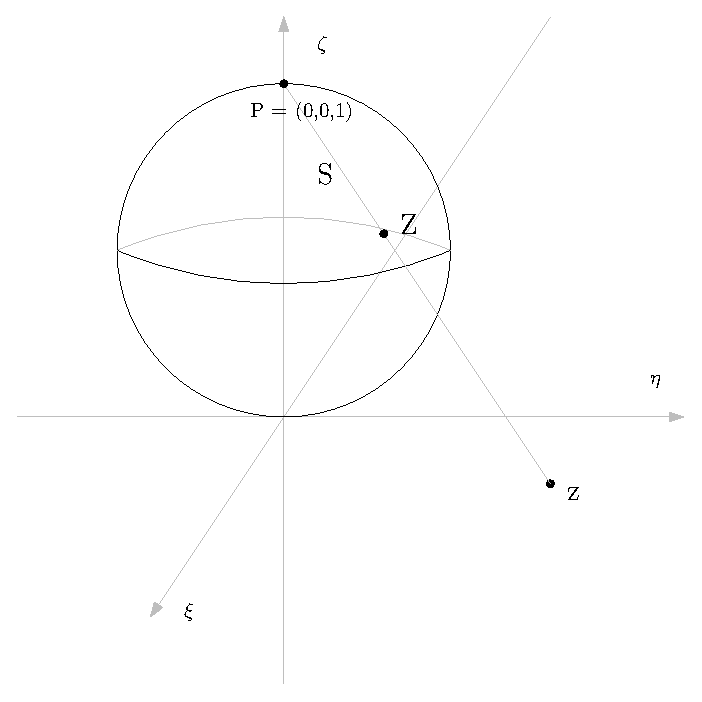
\includegraphics[scale=0.75]{Riemann.eps}
    \caption{Сфера Римана}
		\label{fig:2.1}
\end{figure}
\Def
\textbf{Стереографическая проекция:}
\begin{align*}
  & \forall z \in \CC \ \exists Z \in (\xi, \eta, \zeta): \ \left\{ \begin{matrix}
          \xi = tx \\
          \eta = ty \\
          \zeta = 1-t
      \end{matrix} \right., \ t \in [0;1]
\end{align*}
\begin{align*}
  & t = \frac{1}{1+ \left| z \right|^2}, \ \xi = \frac{x}{1+ \left| z \right|^2}, \ \eta = \frac{y}{1+ \left| z \right|^2}, \ \zeta = \frac{\left| z \right|^2}{1+ \left| z \right|^2}
\end{align*}
\begin{align*}
  & S \setminus P \leftrightarrow \CC, \ P \leftrightarrow \infty
\end{align*}
\textbf{Свойства}
\begin{enumerate}
    \item Любая пряая или окружность на комплексной плоскости переходит в
    окружность на сфере Римана.
    \item Если любые две кусочно гладкие кривые $\gamma_1$ и $\gamma_2$
    пересекаются под углом $\alpha$ на комплексной плоскости, то их образы
    $\tilde{\gamma}_1$, $\tilde{\gamma}_2$ будут пересекаться под тем же углом
    $\alpha$ на сфере Римана.
\end{enumerate}
\Def
$f: G \mapsto D$, где $G$~--- область, $D \subseteq \CCC$~--- область или вся
(расширенная) комплексная плоскость; $f(z) = u(x,y) + iv(x,y)$~---
\textbf{функция комплексного переменного.}
\Def
Пусть $z_0$~--- предельная точка $G \subseteq \CCC$ и $f: G \mapsto \CCC$; тогда
число $A$ назыается \textbf{пределом} $f$ в этой точке (пишется $\dst \lim_{z \to
  z_0} f(z_0)$) тогда и только тогда, когда выполняется
\begin{equation}\label{(2.3)}
    \forall \varepsilon > 0 \ \exists \delta(\varepsilon) > 0: \ z \in \os{\circ}{B}_\delta(z_0)\cap G \hookrightarrow f(z) \in B_\varepsilon (A)
\end{equation}
\asm
\begin{align*}
  & \exists \lim_{z \to z_0}f(z) = A = a+ib \Leftrightarrow \left\{ \begin{matrix}
          \dst \lim_{(x,y)\os{G}{\to}(x_0,y_0)}u(x,y) = a \\
          \dst \lim_{(x,y)\os{G}{\to}(x_0,y_0)}v(x,y) = b
      \end{matrix} \right.
\end{align*}
\pr
Очевидно по аналогии с последовательностями.
\Def
$f: G \mapsto \CCC$ \textbf{непрерывна} в $z_0 \in G \subseteq \CCC$, если
$z_0$~--- предельная точка $G$ и $\dst \lim_{z \to z_0} = f(z_0)$.
\asm
Функция непрерывна тогда и только тогда, кода ее действителная и мнимая части
непрерывны.
\pr Очевидно по аналогии с пределом.
\Def
\textbf{Функциональным рядом} называется сумма вида $\dst \sum_{n=1}^\infty
f_n(z)$, где $\forall n \in \NN \ f_n :G \mapsto \CC$.
\Def
Ряд \textbf{сходится равномерно}, если он:
\begin{enumerate}
    \item $\forall z \in G$ сходится к некоторой $S(z)$;
    \item $\forall \varepsilon > 0 \ \exists N(\varepsilon) > 0: \ \forall N \geq N
    (\varepsilon) \ \left| \dst \sum_{n=1}^Nf_n(z) - S(z) \right|\leq
    \varepsilon$.
\end{enumerate}
Все критерии и признаки для таких рядов аналогичны таковым в действительном
анализе.    
    \setcounter{section}{9}
\section{Глава 10. Кратные интегралы}
\subsection{Определение кратного интеграла}
\subsubsection{Случай, когда $f(x)$ - ограниченная функция.}
\begin{Def}
Пусть $f$ -- ограниченная функция, заданная на измеримом по Лебегу Жордану) множестве $E \subset \R^n$ конечной меры. 

$\textbf{Разбиением}$ множества $E$ называется $E=\bigsqcup\limits_{k=1}^N E_k$, где $E_k$ - измеримые по Лебегу (Жордану). \newline В качестве $\Delta x_k$ будем брать меру множеств $E_k$. 

Обозначим $M_k=\sup\limits_{x\in E_k} f\left(x\right) ,\  m_k=\inf\limits_{x\in E_k}f\left(x\right)$ \newline
Суммы Дарбу - Лебега (Жордана): верхняя $\mathcal{U}(P, f)=\sum\limits_{k=1}^N M_k \cdot \mu_{(J)}(E_k)$, нижняя $L(P, f)\?=\sum\limits_{k=1}^N m_k \cdot \mu_{(J)}(E_k)$.
\newline Верхний интеграл Лебега или Римана (L)(R)$\ \overline{I}_E(f)=\inf\limits_P \mathcal{U}(P, f)$,\newline Нижний интеграл Лебега или Римана (L)(R)$\ \underline{I}_E(f)=\sup\limits_P L(P, f)$
\end{Def}
\begin{Def}
Если (R)$\ \overline{I}_E(f)=$ (R)$\ \underline{I}_E(f)$, то $f$ называется интегрируемой по Риману на $E$, $\int\limits_E f(x)dx=$ (R)$\ \overline{I}_E(f)$ \newline
Если (L)$\ \overline{I}_E(f)=$ (L)$\ \underline{I}_E(f)$, то $f$ называется интегрируемой по Лебегу на $E$, $\int\limits_E f(x)d\mu (x)\?= \text{(L) }\overline{I}_E(f)$
\end{Def}
\textbf{Утв. 1} Функция $f$ интегрируема по Риману на $[a,b]$(в смысле старого определения) $\Leftrightarrow$ $f$ интегрируема по Риману на $E=[a,b] \subset \R^1$.
\begin{proof}
$(\Rightarrow)$	Составим цепочку неравенств:
\begin{equation}
\underline{I}(f) \overset{(1)}{\leqslant} \text{(R) }\underline{I}_{[a,b]}(f)\overset{(2)}{\leqslant} \text{(L) }\underline{I}_{[a,b]}(f)\overset{(3)}{\leqslant}\text{(L) } \overline{I}_{[a,b]}(f) \overset{(4)}{\leqslant} \text{(R) } \overline{I}_{[a,b]}(f)\overset{(5)}{\leqslant} \overline{I}(f)\tag{10.1.1}\label{10.1.1} 
\end{equation}

Неравенство (1) следует из того, что в старом определении мы делили на отрезки, которые пересекаются в концах, а в новом определении идет разбиение на непересекающиеся, измеримые по Жордану множества.

Неравенство (2) следует из того, что нижние интегралы в смысле Римана и в смысле Лебега отличаются тем, на какие множества мы разбиваем: измеримые по Жордану или Лебегу. Но так как каждое измеримое по Жордану автоматически измеримо по Лебегу, то в $\text{(L) }\underline{I}_{[a,b]}(f)$ мы берем точную верхнюю грань по большему множеству.

Неравенства (4), (5) следуют из выше доказанных, но в обратном порядке.

Доказательство неравенства (3): хотим установить, что для любых двух разбиений $P_1, P_2\ L(P_1, f) \leqslant \mathcal{U}(P_2, f)$, что и докажет требуемое неравенство. Для этого необходимо взять общее измельчение разбиений $P=P_1 \bigcup P_2$ и получить цепочку неравенств $L(P_1, f) \leqslant L(P, f) \leqslant \mathcal{U}(P, f) \leqslant \mathcal{U}(P_2, f)$. Получим это: составим два произвольных разбиения 
$P_1 : E = \bigsqcup\limits_{k=1}^{N_1} E_k^{(1)},\ P_2 : E = \bigsqcup\limits_{k=1}^{N_2} E_k^{(2)}$. Тогда общее измельчение $ P : E = \bigsqcup\limits_{k=1}^{N_1} \bigsqcup\limits_{j=1}^{N_2} E_k^{(1)} \bigcap E_j^{(2)}$.
Докажем неравенство для нижних сумм:

 $L(P_1, f)=\sum\limits_{k=1}^{N_1} \inf\limits_{x\in E_k^{(1)}}f(x) \cdot \mu_{(J)}(E_k^{(1)}) =
\sum\limits_{k=1}^{N_1} \inf\limits_{x\in E_k^{(1)}}f(x) \sum\limits_{j=1}^{N_2} \mu_{(J)} (E_k^{(1)}\bigcap E_j^{(2)})\?\leqslant \sum\limits_{k=1}^{N_1}\sum\limits_{j=1}^{N_2}\inf\limits_{x\in E_k^{(1)}\bigcap (E_j^{(2)}}f(x)\cdot \mu_{(J)} (E_k^{(1)}\bigcap E_j^{(2)})=L(P,f)$, так как инфимум по $E_k^{(1)}$ не превосходит инфимум по $E_k^{(1)}\bigcap E_j^{(2)}$ для каждого $j$. Аналогично доказывается оставшаяся часть неравенства.

Из доказанного неравенства \ref{10.1.1} следует, что из интегрируемости по Риману в старом смысле, мы получили интегрируемость в новом смысле, так как $\underline{I}(f) = \overline{I}(f)$, а также, что из интегрируемости по Риману следует интегрируемость по Лебегу.

$(\Leftarrow$)
Отступление.
Вспомним критерий интегрируемости:
$$f\in R[a,b] \Leftrightarrow (\forall \varepsilon > 0)(\exists P)\ \mathcal{U}(P, f)-L(P, f)<\varepsilon$$
В доказательстве мы использовали тот факт, что $\overline{I}(f)=\inf\limits_P \mathcal{U}(P, f)$, $\ \underline{I}(f)=\sup\limits_P L(P, f)$, и так как $\mathcal{U}(P, f)-L(P, f)<\varepsilon$, то и $\overline{I}(f) - \underline{I}(f) < \varepsilon$. Эта разность всегда неотрицательная, меньше любого положительного числа, значит равна 0. Вместо интегрируемости по Риману на отрезке можем написать интегрируемость по Риману на любом измеримом по Жордану или Лебегу.

Вернемся к доказательству.

 Пусть функция интегрируема по Риману в новом смысле: $\exists \int\limits_{[a,b]}f(x)dx$, тогда по критерию интегрируемости: $(\forall \varepsilon > 0)(\exists P:[a,b]=\bigsqcup\limits_{k=1}^{N} E_k) \mathcal{U}(P,f)-L(P,f)<\varepsilon$, где $E_k$ - измеримые по Жордану множества. Внутренняя мера Жордана $\mu_{*}^J(E_k)=\sup\limits_{M \subset E_k} |M|$, где $M$ - элементарное множество. Элементарным множеством на прямой является объединение конечного числа промежутков. Тогда 
$$\exists\text{ набор точек } \{a_j^{(k)}, b_j^{(k)}\},\ \bigsqcup\limits_{j=1}^{n_k}[a_j^{(k)}, b_j^{(k)}] \subset E_k,\ \mu_jE_k \backslash \bigsqcup \limits_{j=1}^{n_k}[a_j^{(k)}, b_j^{(k)}]) < \dfrac{\varepsilon}{2\cdot C \cdot N},$$
\mbox{где $|f(x)|\leqslant C$. Возьмем разбиение в старом смысле $Q: a=x_0 < x_1 < \ldots < x_{\nu} = b,$} $\text{где множество точек }\{x_i\}_{i=1}^{\nu} = \{a_j^{(k)}, b_j^{(k)}\}_{j=1}^{n_k},  k=\overline{1,\ldots,N}$.
Оценим $\mathcal{U}(Q, f)-L(Q, f)=\sum\limits_{i=1}^{\nu}(\sup\limits_{[x_{i-1}, x_i]}f(x)-\inf\limits_{[x_{i-1}, x_i]}f(x))\cdot \Delta x_i = \sum\limits_{k=1}^N \sum\limits_{j=1}^{n_k}(\sup\limits_{x\in [a_j^{(k)},b_j^{(k)}]}f(x)-\inf\limits_{x\in [a_j^{(k)},b_j^{(k)}]}f(x) )(b_j-a_j )+\sum\limits_{x\in B}(\sup\limits_{[x_{i-1}, x_i]}f(x)-\inf\limits_{[x_{i-1}, x_i]}f(x))\Delta x_i \leqslant \sum\limits_{k=1}^N(M_k-m_k)\sum\limits_{j=1}^{n_k}(b_j-a_j)+\sum\limits_{i\in B}\ldots \leqslant \sum\limits_{k=1}^N (M_k-m_k)\cdot \mu_{J}(E_k)+2\cdot C\cdot \sum\limits_{i\in B}\Delta x_i < 2\varepsilon$
\end{proof}
.
\begin{wrapfigure}{r}{0.5\linewidth}
	\includegraphics[width=\linewidth]{images/1.png}
\end{wrapfigure}
\begin{Def}
	\mbox{Пусть $ f:E\to\mathbb{R} $} ---  ограниченная измеримая на измеримом по Лебегу множестве \mbox{$ E\subset\mathbb{R}^n $} конечной меры функция.

	Если $ M=\sup\limits_{x\in E}f(x), $ $ m=\inf\limits_{x\in E}f(x), $ то \textbf{разбиением Лебега}, отвечающим разбиению $ Q=\{m=y_0<y_1<\ldots <y_N=M\}, $ называется разбиение
	$ P: E=\bigsqcup\limits_{i=1}^{N}E_i$, \mbox{где $E_i=\{x\in E: fx)\in [y_{i-1}, y_i)\},$} $i=1, \ldots, N-1$.
	\newline
	$E_N= \{x\in E: fx)\in [y_{N-1}, y_N]\}$
	\newline
	\newline
	\mbox{Тогда интегральной суммой Лебега назовем $S(Q, f, \{t_i\})=\sum\limits_{i=1}^N f(t_i)\mu(E_i)$, где $t_i \in E_i,$}$ 
	\newline i = 1, \ldots, N$.
\end{Def} 
\begin{theorem}(Основная теорема об интеграле Лебега от ограниченных функций).
	Если $f(x)$ ограниченная измеримая на измеримом по Лебегу множестве $ E\subset\R^n $ конечной меры  функция, то она интегрируема по Лебегу (суммируема) на $E$, причем ее интеграл равен пределу интегральных сумм с разбиениями Лебега, отвечающими разбиениям  $ Q $, при стремящемся к нулю диаметре последнего, т.е. $$\int\limits_E f(x)d\mu(x)=\lim_{\Delta(Q)\to 0}S(Q,f,\{t_i\}).$$
	Это значит, что $(\forall \varepsilon >0)(\exists \delta > 0)(\forall Q, \Delta(Q)<\delta) \text{ и } \forall \{t_i\}, t_i \in E_i, i=1,\ldots, N,$ где $E=\bigsqcup\limits_{i=1}^N E_i$ --- разбиение Лебега, отвечающее разбиению $Q$ отрезка $[m, M]$, выполняется $|S(Q, f, \{t_i\})-\int\limits_E f(x)d\mu(x)|<\varepsilon$.
\end{theorem}

\begin{proof}
	Прежде всего заметим, что если $P: E=\bigsqcup\limits_{i=1}^N E_i$, то\newline $L(P, f)\leqslant S(Q, f, \{t_i\})\leqslant \mathcal{U}(P, f)$. Кроме того $\mathcal{U}(P, f) - L(P, f) = \sum\limits_{i=1}^N(M_i-m_i)\mu(E_i) \?\leqslant \sum\limits_{i=1}^N (y_i-y_{i-1})\cdot\mu(E_i)\leqslant \Delta(Q) \sum\limits_{i=1}^N\mu(E_i)=\Delta(Q)\mu(E)$. В качестве $\delta = \dfrac{\varepsilon}{\mu(E)}$. Для множеств $ E $ меры нуль утверждение очевидно, так как все суммы (верхние, нижние, интегральные) в этом случае равны нулю.
\end{proof}

\subsubsection{Случай, когда $f(x)\geqslant 0$.}
Пусть $f(x)\geqslant 0$ - измеримая на измеримом по Лебегу множестве $E$ конечной меры функция. В качестве разбиений будем допускать и разбиения на счетное число измеримых по Лебегу множеств: $E = \bigsqcup\limits_{i=0 }^{\infty}E_i,\ E_0:=\{x\in E:f(x)=+\infty\}$. Обратите внимание! Индексацию ведем с 0, и $E_0$ жестко фиксируем. Соглашение: если $\mu(E_0)=0$, то $(+\infty)\cdot \mu(E_0)=0$. Получаем, что мы ничего не можем сказать о $M$, а $m=0$. 

Тогда разбиение принимает вид $Q: 0=y_0<y_1<\ldots$. 

В качестве $E_i = \{x\in E: f(x)\in[y_{i-1}, y_i)\}, i=1,\ldots$.

$\Delta(Q):=\sup\limits_{i=1, \ldots}(y_i-y_{i-1})$, может равняться и $+\infty$.

$L(P, f)=\sum\limits_{i=0}^{\infty}m_i\cdot \mu(E_i),\  \mathcal{U}(P, f)=\sum\limits_{i=0}^{\infty}M_i\cdot \mu(E_i)$ 

\begin{theorem}Основная теорема об интеграле Лебега для неограниченных измеримых функций)
Если $f(x)$ - неотрицательная, измеримая на измеримом по Лебегу множестве $E\subset \R^n$ конечной меры, то она интегрируема по Лебегу на $E$, причем
$\int\limits_E f(x)d\mu(x)\?=\lim\limits_{\Delta(Q)\to0}S(Q, f, \{t_i\}).$ 

При конечном значении интеграла понятие предела такого вида -- то же, что и в предыдущей основной теореме, если же интеграл бесконечен, то требуется, чтобы \newline$(\forall \varepsilon>0)( \exists \delta > 0)(\forall Q, \Delta(Q)<\delta) \text{ и } \forall \{t_i\}, t_i \in E_i, i=1,\ldots$, где $E=\bigsqcup\limits_{i=1}^{\infty} E_i$ --- разбиение Лебега, отвечающее разбиению $Q$ полуоси $[0, +\infty)$, выполняется $S(Q, f, \{t_i\})\geqslant\varepsilon$.
\end{theorem}

\begin{proof}
В случае конечного интеграла, доказательство аналогично доказательству предыдущей теоремы. Если интеграл бесконечен, то и предел интегральных сумм бесконечность, так как все $S$ зажаты между $\mathcal{U}(P, f) \:\text{и} \:L(P, f)$.
\end{proof}

\begin{Def}
Если $\int\limits_E f(x)d\mu(x) < +\infty$, то $f$ называется суммируемой на $E$.
\end{Def}

\subsubsection{Случай, когда $f(x)$ - любого знака.}
Пусть $f(x)$ измерима на измеримом по Лебегу множестве $E \subset \R^n$ конечной меры. Введем $f_+(x):=\max(f(x), 0), f_-(x):=\max(-f(x), 0)$ - это неотрицательные, измеримые функции. Такие функции интегрируемы по Лебегу, то есть существуют $\int\limits_E f_+(x)d\mu(x), \int\limits_E f_-(x)d\mu(x)$. Если хотя бы один из этих интегралов конечен, то $f$ называется интегрируемой по Лебегу. Если оба конечны, то $f$ - суммируемая на $E$.
$$\int\limits_E f_+(x)d\mu(x)- \int\limits_E f_-(x)d\mu(x) = \int\limits_E f(x)d\mu(x)$$
Пример измеримой, но не интегрируемой по Лебегу функции: возьмем отрезок, на одной его половине функция равна $+\infty$, на другой $-\infty$.



    \section{Лекция 3. Недетерминированные конечные автоматы.}

Вспомним формальное определение (\ref{eq:FA}) конечного автомата.

\textbf{\text{Конечный автомат }} $\mathcal{A}$ --- устройство, описываемое набором $\langle Q$, $\Sigma$, $q_0$, $\delta$, $F \rangle$:
\begin{enumerate}
  \item {\bfseries\itshape{Q}} - конечное множество состояний автомата;
  \item $\boldsymbol{\Sigma}$ - алфавит, слова над которым обрабатывает автомат;
  \item $\boldsymbol{q_0}$ - начальное состояние автомата;
  \item $\boldsymbol{\delta}$ : $Q \times (\Sigma\cup\{\varepsilon\} ) \rightarrow 2^{Q}$ - функция переходов
  \item $\boldsymbol{F} \subset \boldsymbol{Q}$ - множество принимающих состояний.
\end{enumerate}


\begin{wrapfigure}{r}{0.3\textwidth}
  \centering
  \begin{tikzpicture}[node distance=2cm,on grid,auto]
    \node[state,initial] (q_0)   {$q_0$};
    \node[state,accepting] (q_1) [right=of q_0] {$q_1$};
    \path[->]
    (q_0) edge [bend left] node {$b$} (q_1)
    (q_0) edge [loop above] node {$a,b$} ()
    (q_1) edge [bend left] node {$\varepsilon$} (q_0);
  \end{tikzpicture}
  \caption{Пример НДА.}
  \label{fig:NFAexample}
\end{wrapfigure}

Рассмотрим рисунок (\ref{fig:NFAexample}). К примеру сразу из определения и графа имеем: $\delta(q_0,\:b)=\{q_0,q_1\}$.

\begin{question}
  Неформально опишите язык, распознаваемый данным автоматом.
\end{question}

\begin{nonum}
  Язык $R$, состоящий из слов, оканчивающихся на $b$.

  В самом деле, в принимающее состояние можно перейти по единственному переходу на котором написан символ $b$, то есть $L(\mathcal{A})\subseteq R$.
  Далее любое слово, оканчивающееся на $b$ принимается автоматом, потому что, обрабатывая все символы слова автомат может оставаться в состояний
  $q_0$, а когда встретится последний символ(он же буква $b$) перейти в состояние $q_1$. Итак, $R\subseteq L(\mathcal{A})$.
\end{nonum}

\subsection{Алгоритм проверки принадлежности слова языку, распознаваемому НКА.} \label{alg:word}

В случае ДКА все тривиально. Просто эмулируем работу автомата на входном слове. Каждое следующее состояние определяется однозначно.
Обработав слово за линейное время выясняем принимается ли оно автоматом.

В случае НКА может быть несколько путей вычесления, к примеру для слова $bb$ в автомате на рисунке (\ref{fig:NFAexample})
есть более одного пути: $$q_0\xrightarrow{b} q_0\xrightarrow{b} q_1,$$
$$q_0\xrightarrow{b} q_1\xrightarrow{\varepsilon} q_0\xrightarrow{b} q_0.$$

Заметим, что не обязательно все возможные пути заканчиваются в принимающем(или не принимающем) состоянии, в приведенном примере один путь
заканчивается, другой --- нет.

\paragraph*{Алгоритм.} Пусть есть слово $w = w_1w_2\ldots w_n$, $w_i\in\Sigma^*$. На $i$"=ом шаге будем помнить и пересчитывать множество состояний
$Q_i=\{q\:|\:q_0\xrightarrow{w[1,i]}q\}$.

Итак, если после обработки слова, в $Q_n$ есть принимающее состояние, то слово принимается.
Для более формального описания алгоритма, введем функцию
$$\varepsilon\text{-closure}(S)=S\cup \{q\:|\:\exists p\in S\: :\: p\xrightarrow{\varepsilon}q\}$$

Наконец, опишем алгоритм формально:

\begin{enumerate}
  \item Построить множество $Q_0$ = $\varepsilon$"=closure($q_0$).
  \item Для $k$ от 1 до $|w|$ построить множества:
        \begin{itemize}
          \item $Q_k'=\{p\:|\:\exists q\in Q_k\: :\: p\in\delta(q,\:w_k)\}$;
          \item $Q_{k+1}=\varepsilon\text{-closure}(Q_k')=\displaystyle{\bigcup _{q'\in Q_k'}}\varepsilon\text{-closure}(q')$;
        \end{itemize}
  \item Если $Q_{|w|}\cap F_{\mathcal{A}}\neq \varnothing$, то ответ <<Да>>, иначе <<Нет>>.
\end{enumerate}


\begin{question}
  Как эффективно вычислить $\varepsilon\text{-closure}(S)$?
\end{question}

\begin{nonum}
  Рассмотрим подграф графа автомата, в котором оставлены только ребра, на которых написано $\varepsilon$.
  И дальше для каждого состояния из $S$ обходом в глубину(или в ширину) будем искать все достижимые состояния.
\end{nonum}


\subsection{Построение НКА по РВ.}

Напомним, что по определению любой регулярный язык
можно построить согласно следующей схеме:

\begin{enumerate}
  \item $\varnothing \in REG$
  \item $\forall\sigma \in \sum \implies \{\sigma\} \in  REG$
  \item $\forall X, Y \in REG: X \circ Y, X|Y, X^* \in REG$
\end{enumerate}

Мы будем строить НКА по РВ для каждого пункта. Более того,
нам потребуется соблюсти технические условия:

\begin{enumerate}[(i)]
  \item НКА имеет ровно одно принимающее состояние;
  \item В начальное состояние НКА не ведёт ни один переход;
  \item Из принимающего состояния НКА нет ни одного перехода.
\end{enumerate}

\begin{question}
  Построить такой автомат для
  \begin{itemize}
    \item Пустого языка;
    \item Языка, состоящего из одного символа.
  \end{itemize}
\end{question}


\begin{nonum}
  Приведем только ответы, корректность очевидна.

  \begin{figure}[!h]
    \centering
    \begin{minipage}{.5\textwidth}
      \centering
      \begin{tikzpicture}[node distance=2cm,on grid,auto]
        \node[state,initial] (q_0)   {$q_0$};
        \node[state,accepting] (q_1) [right=of q_0] {$q_1$};
      \end{tikzpicture}
      \caption{Пустой язык.}
    \end{minipage}%
    \begin{minipage}{.5\textwidth}
      \centering
      \begin{tikzpicture}[node distance=2cm,on grid,auto]
        \node[state,initial] (q_0)   {$q_0$};
        \node[state,accepting] (q_1) [right=of q_0] {$q_1$};
        \path[->]
        (q_0) edge node {$a$} (q_1);
      \end{tikzpicture}
      \caption{Язык $\{a\}$.}
    \end{minipage}
  \end{figure}
\end{nonum}


Осталось построить автоматы для пункта (3) определения регулярного языка. Будем изображать НКА схематично, помечая в них только начальное и принимающее состояния:
\begin{figure}[!h]
  \centering
  \begin{tikzpicture}[node distance=2cm,on grid,auto]
    \draw (0.5,0) ellipse (3cm and 1.5cm);
    \node[state,initial] (q_0)   {$q_0$};
    \node[] at (1,0) {$\mathcal{A}$};
    \node[state,accepting] (q_1) [right=of q_0] {$q_1$};
  \end{tikzpicture}
  \caption{Автомат, удовлетворяющий условиям (i–iii).}
\end{figure}

Далее, мы будем предполагать, что начальное состояние на схеме
находится слева, а принимающее справа.
Допустим уже построены автоматы $\mathcal{A}$ и $\mathcal{B}$ (удовлетворяющие условиям (i–iii)) для регулярных языков
$X$ и $Y$ соответственно. Построим
явно автомат, распознающий $X \cdot Y$.

\begin{figure}[!ht]
  \centering
  \begin{tikzpicture}[node distance=4.5cm,on grid,auto,initial text=]
    \draw (1,0) ellipse (2cm and 1cm);
    \draw (3.5,0) ellipse (2cm and 1cm);
    \draw (2.25, 0) circle (0.5cm);
    \node[state,initial] (q_0)   {$q_0^{\mathcal{A}}$};
    \node[state,accepting] (q_1) [right=of q_0] {$q_F^{\mathcal{B}}$};
    \node[] at (1,0) {$\mathcal{A}$};
    \node[] at (3.5,0) {$\mathcal{B}$};
  \end{tikzpicture}
  \caption{Автомат для конкатенации.}
  \label{fig:concatFA}
\end{figure}

Как видно из рисунка \ref{fig:concatFA}, результирующий автомат получен из автоматов $\mathcal{A}$ и $\mathcal{B}$
следующим образом. Начальное состояние автомата $\mathcal{B}$
\textit{склеено} с начальным состоянием автомата $\mathcal{A}$:
мы удалили из автомата $\mathcal{B}$ начальное состояние $q_0^{\mathcal{B}}$, а все переходы, которые вели из него,
добавили к принимающему состоянию $q_F^{\mathcal{A}}$
автомата $\mathcal{A}$, которое сделали непринимающим.
Дабы определить склейку состояний для произвольных автоматов, скажем, что если бы в состояние $q_0^{\mathcal{B}}$ вели какие-то
переходы, то их бы также направили в состояние, полученное в результате склейки.


Далее строим автомат для языка $X | Y$ используя конструкцию:

\begin{figure}[!ht]
  \centering
  \begin{tikzpicture}[node distance=3cm,on grid,auto,initial text=]
    \node[state,initial] (q_0)   {$q_0$};
    \node[state] (q_0a) [above right=of q_0] {$q_0^{\mathcal{A}}$};
    \node[state] (q_fa) [right=of q_0a] {$q_F^{\mathcal{A}}$};
    \node[state] (q_f) [below right=of q_fa] {$q_F$};
    \node[state] (q_0b) [below right=of q_0] {$q_0^{\mathcal{B}}$};
    \node[state] (q_fb) [right=of q_0b] {$q_F^{\mathcal{B}}$};
    \node[] at (3.6, 2.1) {$\mathcal{A}$};
    \node[] at (3.6, -2.1) {$\mathcal{B}$};
    \draw (3.6, 2.1) ellipse (2.5cm and 1cm);
    \draw (3.6, -2.1) ellipse (2.5cm and 1cm);
    \path[->]
    (q_0) edge node {$\varepsilon$} (q_0a)
    (q_0) edge node {$\varepsilon$} (q_0b)
    (q_fa) edge node {$\varepsilon$} (q_f)
    (q_fb) edge node {$\varepsilon$} (q_f);
  \end{tikzpicture}
  \caption{Автомат для конкатенации.}
  \label{fig:sumFA}
\end{figure}


И наконец перейдём к построению автомата для языка $X^*$:


\begin{figure}[!ht]
  \centering
  \begin{tikzpicture}[node distance=2.5cm,on grid,auto,initial text=]
    \node[state,initial] (q_0)   {$q_0$};
    \node[state] (q_0a) [right=of q_0] {$q_0^{\mathcal{A}}$};
    \node[state] (q_fa) [right=of q_0a] {$q_F^{\mathcal{A}}$};
    \node[state] (q_f) [right=of q_fa] {$q_F$};
    \draw (3.75,0) ellipse (2cm and 1cm);
    \node[] at (3.75,-0.5) {$\mathcal{A}$};
    \path[->]
    (q_0) edge node {$\varepsilon$} (q_0a)
    (q_0) edge [bend left] node {$\varepsilon$} (q_f)
    (q_fa) edge [bend right] node {$\varepsilon$} (q_0a)
    (q_fa) edge node {$\varepsilon$} (q_f);
  \end{tikzpicture}
  \caption{Автомат $C$ для итерации.}
  \label{fig:iterFA}
\end{figure}


\begin{proof}

  По индукции докажем, что для $\forall n>0$ $w\in X^n\Rightarrow w\in L(C)$, то есть докажем включение $X^*\subseteq L(C)$.

  \underline{База}: пустое слово принимается автоматом.

  \underline{Переход}: Рассмотрим слово $w=u_1\cdot u_2\cdot\ldots\cdot u_n$, $u_i\in L(\mathcal{A})$. Слово
  $v=u_1\cdot u_2\cdot\ldots\cdot u_{n-1}\in L(C)$ по предположению индукции. Есть несколько вариантов.
  \begin{itemize}
    \item $v$ --- пустое. Но тогда можно попасть в состояние $q_0^{\mathcal{A}}$, а из него, так как $u_n$ принимается $\mathcal{A}$,
          в состояние $q_F^{\mathcal{A}}$, откуда уже в $q_F$.
    \item $v$ --- непустое. Это означает, что путь по нему из начального состояния в принимающее обязательно прошел через
          $q_F^{\mathcal{A}}$. Тогда вернемся на шаг назад в состояние $q_F^{\mathcal{A}}$, а из него еще на шаг в состояние
          $q_0^{\mathcal{A}}$ по ребру $\varepsilon$. И оттуда уже обрабатываем слово $u_n$.
  \end{itemize}

  Теперь докажем $L(C)\subseteq X^*$.

  Пусть слово $w\in L(c)$. Если $w$ --- пустое, то оно очевидно принадлежит $X^*$. Если же слово не пустое, посмотрим на путь из $q_0$.
  Если этот путь не проходил через ребро $q_F^{\mathcal{A}}\xrightarrow{\varepsilon} q_0^{\mathcal{A}}$, тогда все очевидно.

  Если же этот переход был, найдем первый этот переход, который случился после того, как был обработан какой-то непустой префикс слова $w$.
  Заметим, что этот префикс есть собственный префикс $w$ и по предположению индукции этот префикс принадлежит $X^*$. Заметим, что и суффикс принадлежит
  $X^*$, но тогда и $w$ принадлежит $X^*$.

\end{proof}


\subsection{Построение ДКА по НКА.}

Модифицируем алгоритм проверки принадлежности слова языку, распознаваемому НКА. Заметим, что число множеств $Q_k$,
появлявшихся в алгоритме, конечно, поскольку $Q_k \subseteq 2^{Q_{\mathcal{A}}}$. Поэтому всевозможные множества
можно хранить в конечной памяти, они и будут состояниями ДКА, который мы назовём $2^{\mathcal{A}}$.
Начальным состоянием будет состояние $Q_0$,
принимающими будут множества $Q_k$, содержащие принимающие состояния $\mathcal{A}$, а переходы между состояниями определены, как и в алгоритме:

\begin{enumerate}
  \item $Q_0 = \varepsilon\text{-closure}(q_0)$
  \item $\delta (Q', a)=\varepsilon\text{-closure}(\widetilde{Q}')$, где
        $\widetilde{Q}'=\{q\:|\: \exists p\in Q':\:p\in\delta(p, a)\}=\displaystyle{\bigcup_{p\in Q'}}\delta(p, a).$
\end{enumerate}


\subsection{Построение РВ по НКА.}

\begin{Def}
  \textit{Обобщенный НКА} --- НКА, у которого вместо букв на переходах написаны регулярные выражения.

  Слово $w\in L(\mathcal{A})$, если существует разбиение $w=u_1\cdot u_2\cdot\ldots\cdot u_n$, $u_i\in \Sigma^*$ и существует
  последовательность состояний $q_1, q_2, \ldots, q_n\in F$, такие что $u_1\in R_{q_0, q_1}$, $u_2\in R_{q_1, q_2}$, \ldots, $u_n\in R_{q_{n-1}, q_n}$, где
  $R_{q_i,q_j}$ --- РВ написанное на ребре $q_i\rightarrow q_j$.
\end{Def}

Основная идея такая. Вначале нужно превратить НКА в НКА с одним принимающем состоянием, в который не ведет ни одно ребро и с начальным состоянием
в которое также ничего не ведет (рисунок (\ref{fig:prepare})).

\begin{figure}
  \centering
  \begin{tikzpicture}[node distance=3cm,on grid,auto,initial text=]
    \node[state,initial] (q0)   {$q_0$};
    \node[state, initial] (q1) at (1,3) {};
    \node[state,accepting] (p) at (5, 0) {$p$};
    \node[state,accepting] (r1) at (4.5, 2.5) {};
    \node[state,accepting] (r2) at (3, 2) {};
    \node[state,accepting] (r3) at (5, 4) {};
    \draw (3,3) ellipse (4cm and 2cm);
    \path[->]
    (q0) edge node {$\varepsilon$} (q1)
    (r1) edge node {$\varepsilon$} (p)
    (r2) edge node {$\varepsilon$} (p)
    (r3) edge [bend left, out=30, in=120] node {$\varepsilon$} (p);
  \end{tikzpicture}
  \caption{Начальная подготовка графа.}
  \label{fig:prepare}
\end{figure}


Далее делаем старые принимающие состояние непринимающими и переходим к следующему шагу.

Берем НКА и последовательно удаляем состояния, пересчитывая ребра.

\begin{wrapfigure}{r}{0.45\textwidth}
  \centering
  \begin{tikzpicture}[node distance=2.5cm,on grid,auto,initial text=]
    \node[state,initial] (q)   {$q$};
    \node[state] (p) [right=of q] {$p$};
    \node[state] (r) [right=of p] {$r$};
    \path[->]
    (q) edge node {$R_{q,p}$} (p)
    (p) edge node {$R_{p,r}$} (r)
    (p) edge [loop above] node {$R_{p,p}$} ()
    (q) edge [bend right, in=240] node {$R_{q,r}$} (r);
  \end{tikzpicture}
  \caption{Удаление состояния.}
  \label{fig:deleteNode}
\end{wrapfigure}


Допустим нужно удалить состояние $p$. Нужно рассмотреть все пары $(q, r)$ удовлетворяющие
рисунку (\ref{fig:deleteNode}).
Тогда после удаления $p$ нужно убрать все ребра на рисунке и добавить ребро $q\xrightarrow{R'_{q, r}}r$, где $$R'_{q,r}=R_{q,r}\cup R_{q,p}R^*_{p,p}R_{p,r}$$.

    \begin{flushright}
    \textit{Лекция 4 (от 15.09)}
\end{flushright}

\textbf{Кривая} $\gamma$~--- класс эквивалентных параметризаций $z(t) = x(t) +
iy(t), \ t \in \left[ t_0; t_1 \right]$
\\
\textbf{Параметризации эквивалентны}, если существует монотонная возрастающая
функция $\psi(\tau) = t$, сохраняющая направление.
\\
\textbf{Гладкая кривая (ГК)}~--- такая кривая $\gamma$, что существует параметризация
$z(t) = x(t) + iy(t)$, $x \in C^1 \left( \left[ t_0; t_1 \right] \right)$, $y
\in C^1 \left( \left[ t_0; t_1 \right] \right)$, $\forall t \in \left[ t_0; t_1
\right] \ z'(t) \neq 0$.
\\
\textbf{Замкнутая ГК (ЗГК)}~--- такая ГК, что $z(t_0) = z(t_1)$, $z'(t_0+0) =
z'(t_1-0)$.
\\
\textbf{Кусочно гладкая кривая (КГК)}~--- такая непрерывная кривая $\gamma$, что
$\exists t_0 = \theta_0 < \theta_1 < \dots < \theta_{n-1} < \theta_n = t_1$, что
$\forall k \ \gamma_k: \ z(t), \ t \in [\theta_{k-1}, \theta_k]$ есть ГК.
\\
\textbf{Разбиение} отрезка $\left[ t_0, t_1 \right]$: $\lambda = \{t_0 = \tau_0
< \tau_1 < \dots < \tau_{m_\lambda} = t_1\}$.
\\
\textbf{Мелкость (диаметр)} разбиения $\lambda$ $\left| \lambda \right| = \dst
\max_{k \{1, \dots, m_\lambda\}}\left| \tau_k - \tau_{k-1} \right|$.
\Def Пусть $f: \gamma \mapsto \CC$ непрерывна на КГК $\gamma$. Пусть
$\lambda$~--- разбиение $\left[ t_0, t_1 \right]$ для $\gamma: \ z(t)$~---
кусочно гладкой. Пусть $z(t_k) = z_k, \ k \in \{0, \dots, m_\lambda\}$, $\zeta_k
\in \gamma_k = \gamma_{z_{k-1}z_k}$
\begin{align*}
  & \sigma(\lambda) = \sum_{k = 1}^{m_{\lambda}} f(\zeta_k) \Delta z_k
\end{align*}
$\Delta z_k = z_k - z_{k-1}$~--- \textbf{интегральная сумма};
\\
если $\exists \lim \sigma(\lambda) \ \forall \zeta_k, \ \left| \lambda \right|
\to 0$, то этот предел называется \textbf{интегралом Римана от $f$ по $\gamma$}
и записывается как
\begin{equation} \label{(6.1)}
    \int_{\gamma}f(z) dz
\end{equation}
\theorem
Если условия определения интеграла выполняются, то он существует и справедливо:
\begin{equation} \label{(6.2)}
    \int_{\gamma}f(z)dz = \int_{\gamma}\left( u dx - v dy \right) + i \int_\gamma \left( v dx + u dy \right)
\end{equation}
\pr
\begin{align*}
  & \sigma(\lambda) = \sum_{k = 1}^{m_\lambda}\left( u(\xi_k, \eta_k) + iv(\xi_k, \eta_k) \right)\left( \Delta x_k + i \Delta y_k \right) = \sum_{k = 1}^{m_\lambda}\left( u(\xi_k, \eta_k) \Delta x_k - v(\xi_k, \eta_k) \Delta y_k\right) + \\
  & + \left( v(\xi_k, \eta_k) \Delta x_k + u(x_k, y_k) \Delta y_k\right) = \sigma_1(\lambda) + \sigma_2(\lambda) \to \int_{\gamma}\left( u dx - v dy \right) + i \int_\gamma \left( v dx + u dy \right)
\end{align*}
\corollary
Если условия определения интеграла выполняются, то верно:
\begin{equation} \label{(6.3)}
    \int_\gamma f(z) dz = \int_{t_0}^{t_1}f(z(t))z'(t)dt
\end{equation}
\begin{equation} \label{(6.4)}
    \gamma: z(t), \ \int_{t_0}^{t_1}\left( P(t) + iQ(t) \right) dt = \int_{t_0}^{t_1}P(t)dt + i \int_{t_0}^{t_1}Q(t)dt
\end{equation}
\pr
Из \eqref{(6.2)} и свойств криволинейных интегралов II рода
\begin{align*}
  &\int_{\gamma}P(x,y) dx + Q(x,y)dy = \int_{t_0}^{t_1} \left( P(x(t), y(t))x'(t) + Q(x(t), y(t))y'(t) \right) dt
\end{align*}
\underline{\textbf{Общие свойства интеграла}}
\begin{enumerate}
    \item Линейность:
    \begin{align*}
      &\int_{\gamma}\left(\lambda f(z) + \mu g(z)\right) dz = \lambda\int_{\gamma}f(z) dz + \mu \int_\gamma g(z) dz
    \end{align*}
    \item Аддитивность вдоль кривой: если $\gamma = \gamma_1 \cup \gamma_2$
    (общая точка~--- только конец), то
    \begin{align*}
      &\int_{\gamma}f(z) dz = \int_{\gamma_1}f(z) dz + \int_{\gamma_2} f(z) dz
    \end{align*}
    \item Изменение знака при смене направления: если $\gamma^{-1}$~---
    кривая, совпадающая во всех точках с $\gamma$, но противоположно
    направленная, то
    \begin{align*}
      &\int_{\gamma^{-1}}f(z) dz = - \int_{\gamma}f(z) dz
    \end{align*}
    \item Инвариантность относительно замены параметра.
    \item Выполняется неравенство:
    \begin{equation} \label{(6.5)}
        \left| \int_\gamma f(z) dz \right| \leq \int_{\gamma}\left| f(z) \right| \cdot \left| dt \right| = \int_{t_0}^{t_1} \left| f(z(t)) \right| \sqrt{(x'(t))^2 + (y'(t))^2}dt
    \end{equation}
    \pr
    Из \eqref{(6.3)}:
    \begin{equation} \label{(6.6)}
        \left| \sigma(\lambda) \right| \leq \sum_{k = 1}^{m_\lambda}\left| f(\zeta) \right| \cdot \left| \Delta z_k \right|
    \end{equation}
\end{enumerate}
\example
\begin{align*}
  &J_k = \int_{\gamma: \left| z-a \right| = r} (z-a)^k dz, \ k \in \ZZ
\end{align*}
Параметр: $z(t)= a+re^{it}, \ t \in [0;2\pi]$
\begin{align*}
  & dz(t) = rie^{it}dt
\end{align*}
\begin{align*}
  &J_k = \int_{0}^{2\pi} r^ke^{ikt}rie^{it}dt = r^{k+1}i\int_{0}^{2\pi}e^{i(k+1)t} dt
\end{align*}
\begin{align*}
  &J_{-1} = 2 \pi i
\end{align*}
\begin{align*}
  &J_k = r^{k+1}i\int_{0}^{2\pi} \left( \cos(k+1)t + i \sin(k+1)t \right) dt = 0, \ k \neq -1
\end{align*}
\example
\begin{align*}
  &J_1 = \int_{\gamma} dz, \ J_2 = \int_{\gamma}z dz
\end{align*}
$\gamma: z(t)$, и согласно \eqref{(6.3)}
\begin{align*}
  &J_1 = \int_{t_0}^{t_1} z'(t)dt = z(t_1) - z(t_0)
\end{align*}
\begin{align*}
  &J_2 = \int_{t_0}^{t_1} z(t)z'(t)dt = \frac{1}{2}\int_{t_0}^{t_1}\frac{d}{dt}\left( z^2(t) \right)dt = \frac{1}{2}\left( z^2(t_1) - z^2(t_0) \right)
\end{align*}
\theorem
Пусть $f_n: G \mapsto \CC$ непрерывна на $G$ $\forall n \in \NN$, $\gamma$~---
КГК, $\gamma \subseteq G$.
\\
Пусть $\dst \sum_{n=1}^{\infty}f_n(z) \underset{\gamma}{\rightrightarrows} S(z)
\ \forall z \in \gamma$.
Тогда $S(z)$ непрерывна на $\gamma$ и выполняется
\begin{equation} \label{(6.7)}
    \int_{\gamma}S(z) dz = \sum_{n=1}^{\infty}\int_{\gamma}f_n(z)dz
\end{equation}
\pr
Ряд сходится равномерно на $\gamma$
\begin{align*}
  & \Updownarrow
\end{align*}
\begin{equation} \label{(6.8)}
    \forall \varepsilon > 0 \ \exists N(\varepsilon): \ \forall N\geq N(\varepsilon) \ \underset{z \in \gamma}{\sup} \left| S(z) - \sum_{n = 1}^{N}f_n(z) \right| = \underset{z \in \gamma}{\sup} \abs{S - S_N(z)} \leq \varepsilon
\end{equation}
\begin{align*}
  &\exists \delta > 0: \ \forall z_0 \in \gamma, \ z \in \gamma, \ \left| z - z_0 \right| < \delta: \ \left| S(z) - S(z_0) \right| \leq \left| S(z) - S_N(z) \right| +  \left| S_N(z) - \right. \\
  &\left. - S_N(z_0) \right| + \left| S_N(z_0) - S(z_0) \right| \leq \left| S_N(z) - S_N(z_0) \right| + 2 \varepsilon \leq 3 \varepsilon
\end{align*}
\begin{align*}
  & \Downarrow
\end{align*}
\begin{align*}
  & S(z) \rightarrow S(z_0)
\end{align*}
\begin{align*}
  & \Downarrow
\end{align*}
\begin{align*}
  & \exists \int_{\gamma}S(z)dz
\end{align*}
\begin{align*}
  &\forall N \geq N(\varepsilon) \ \left| \int_{\gamma}S(z)dz - \int_{\gamma}S_N(z)dz\right| = \left| \int_\gamma \left( S(z) - S_N(z) \right)dz\right| \leq \int_\gamma \left| S(z) - S_N(z) \right| \left| dz \right| \leq \\
  & \leq \varepsilon \int_{\gamma} \left| dz \right| = \varepsilon l(\gamma) = \varepsilon \cdot const
\end{align*}
Теорема доказана.
\Def
Пусть $g: G \mapsto \CC$ на области $G$; назовем это \textbf{первообразной}
непрерывной функции $f: G \mapsto \CC$, если $g$ регулярна на $G$ и $g'(z) =
f(z) \ \forall z \in G$.
\Def
Выражение $f(z)dz$ называется \textbf{полным дифференциалом в области $G$}, если
существует первообразная $g$ для $f$ на $G$, т.~е. $f(z)dz = g'(z)dz$.
\theorem
Пусть $f:G \mapsto \CC$ непрерывна на области $G$. Тогда:
\begin{enumerate}
    \item если $f dz$~--- полный дифференциал на $G$, то для любой замкнутой КГК
    $\overset{\circ}{\gamma} \subseteq G$ выполняется
    \begin{equation} \label{(6.9)}
        \int_{\overset{\circ}{\gamma}} f(z) dz = 0
    \end{equation}
    \item если для любой замкнутой ломаной кривой $\gamma$ выполняется
    \eqref{(6.9)}, то $f dz$~--- полный дифференциал.
\end{enumerate}
\pr ~
\\
\begin{enumerate}
    \item $\exists g:G \mapsto \CC$, регулярная, такая, что $g'(z) = f(z)$.
    Тогда
    \begin{align*}
      & \int_{\overset{\circ}{\gamma}} f(z) dz \underset{\overset{\circ}{\gamma}: z = z(t)}{=} \int_{t_0}^{t_1} g'(z(t))z'(t)dt = \int_{t_0}^{t_1}\frac{d}{dt}(g(z(t)))dt = g(z(t_1)) - g(z(t_0)) = \\
      & = g(z(t_1)) - g(z(t_1)) = 0
    \end{align*}
    \item Фиксируем $a \in G$ как начальную точку ломаной $\gamma$. $\forall z
    \in G$ $\exists \gamma_{az}$~--- ломаная с началом в $a$ и концом в $z$.
    \begin{align*}
      & g(z) = \int_{\gamma_{az}} f(z) dz
    \end{align*}
    не зависит от $\gamma_{az}$, а лишь зависит от $z$. Действительно, если
    $\exists \gamma_{az}, \ \exists \tilde{\gamma_{az}}$, то пусть
    $\overset{\circ}{\gamma} = \gamma_{az} \cup \tilde{\gamma_{az}}^{-1}$,
    тогда из \eqref{(6.8)}
    \begin{align*}
      & \int_{\overset{\circ}{\gamma}} f(z) dz = 0 = \int_{\gamma_{az}}f dz - \int_{\tilde{\gamma_{az}}}f(z)dz
    \end{align*}
    Докажем, что $\forall z \ g'(z) = f(z)$. Рассмотрим $z_0$; $\exists
    \varepsilon > 0: B_{\varepsilon}(z_0) \subseteq G$, $\Delta z: 0 <
    \left| \Delta z \right| < \varepsilon$. Тогда $z_0 + \Delta z \in G$.
    Рассмотрим
    \begin{align*}
      & \frac{g(z_0+\Delta z) - g(z_0)}{\Delta z}
    \end{align*}
    Тогда
    \begin{align*}
      & g(z+ \Delta z) = \int_{\gamma_{az_0} \cap [z_0; \Delta z + z_0]}
    \end{align*}
    \begin{align*}
      & \Downarrow
    \end{align*}
    \begin{align*}
      & \frac{g(z_0+ \Delta z) - g(z_0)}{\Delta z} = \frac{1}{\Delta z} \int_{[z_0; \Delta z + z_0]} f(z)dz
    \end{align*}
    \begin{align*}
      & \left| \frac{\Delta g}{\Delta z} - f(z_0) \right| = \left| \frac{1}{\Delta z} \int_{[z_0; \Delta z + z_0]}(f(z) - f(z_0))dz \right|
    \end{align*}
    В силу непрерывности $f(z)$, полагая $r(\varepsilon)$~--- радиус шара, где
    $\left| f(z) - f(z_0) \right| < \varepsilon$,
    \begin{align*}
      & \forall z \in B_{r(\varepsilon)}(z_0)\cap B_\varepsilon(z_0) \ \left| \frac{\Delta g}{\Delta z} - f(z_0) \right| \leq \left| \frac{\varepsilon\min\left\{ r(\varepsilon), \varepsilon \right\}}{\min\left\{ r(\varepsilon), \varepsilon \right\}} \right| = \varepsilon
    \end{align*}
\end{enumerate}

    \begin{proof}
	Имеем множество $E$ необязательно конечной меры, $E=\bigsqcup\limits_{k=1}^\infty E_k$, $E_k$ --- измеримые по Лебегу множества, дополнительно предположим, что $f(x)\geqslant 0$. Хотим установить равенство $\int\limits_{E}f(x)d\mu(x)=\sum\limits_{k=1}^\infty \int\limits_{E_k}f(x)d\mu(x)$.
	
	Возьмем исчерпывание множествами конечной меры $E^{(1)}\subset E^{(2)}\subset \ldots,$ такими, что $\lim\limits_{s\to\infty}E^{(s)}=\bigcup\limits_{s=1}^\infty E^{(s)}=E$. Тогда по определению
	$$\int\limits_{E}f(x)d\mu(x)=\lim\limits_{s\to\infty}\int\limits_{E^{(s)}}f(x)d\mu(x).$$ Обозначим $a_k^{(s)}:=\int\limits_{E_k\cap E^{(s)}}f(x)d\mu(x)$. Заметим, что $E_k\cap E^{(s)}$ имеет конечную меру и $E_k\cap E^{(1)} \subset E_k\cap E^{(2)}\subset\ldots$, $\bigcup\limits_{s=1}^\infty \left( E_k\cap E^{(s)}\right) = E_k$, тогда $a_k:=\int\limits_{E_k}f(x)d\mu(x)=\lim\limits_{s\to\infty}\int\limits_{E_k\cap E^{(s)}}f(x)d\mu(x)=\lim\limits_{s\to\infty}a_k^{(s)}$.
	Все $a_k^{(s)}$ --- неотрицательные числа, значит по Лемме 10.3.1 имеет место равенство: $\lim\limits_{s\to\infty}\sum\limits_{k=1}^\infty a_k^{(s)}=\sum\limits_{k=1}^\infty a_k$. Получаем $\lim\limits_{s\to\infty}\sum\limits_{k=1}^\infty\int\limits_{E_k\cap E^{(s)}}f(x)d\mu(x)=\sum\limits_{k=1}^\infty\int\limits_{E_k}f(x)d\mu(x)$. В левой части равенства интегрирование при каждом фиксированном $s$ происходит на подмножествах $E^{(s)}$, которое имеет конечную меру, и для множеств конечной меры $\sigma$-аддитивность уже доказана, значит $\sum\limits_{k=1}^\infty\int\limits_{E_k\cap E^{(s)}}f(x)d\mu(x)=\int\limits_{E^{(s)}}f(x)d\mu(x) \Rightarrow \lim\limits_{s\to\infty}\int\limits_{E^{(s)}}f(x)d\mu(x)=\sum\limits_{k=1}^\infty\int\limits_{E_k}f(x)d\mu(x)$, что и требовалось. Обратное утверждение следует из того, что из суммируемости $f(x)$ на каждом $E_k$ и сходимости ряда $\sum\limits_{k=1}^\infty\int\limits_{E_k}f(x)d\mu(x)$ следует суммируемость функции $f$ на $E$.
	
	Рассмотрим случай функции любого знака. Представим $f = f^+ - f^-$, для каждой из этих функций справедливо выше доказанное свойство: $\int\limits_{E}f^\pm(x)d\mu(x)=\sum\limits_{k=1}^\infty \int\limits_{E_k}f^\pm(x)d\mu(x)$, и взяв разность рядов, получаем $\sigma$-аддитивность для функций любого знака. Обратное утверждение следует из того, что из сходимости ряда $\sum\limits_{k=1}^\infty\int\limits_{E_k}|f(x)|d\mu(x)$, следует сходимость рядов $\sum\limits_{k=1}^\infty \int\limits_{E_k}f^\pm(x)d\mu(x)$, а значит $f^+$ и  $f^-$ суммируемы на $E$, то есть $f$ суммируема на $E$.
\end{proof}

\begin{prop}[Абсолютная непрерывность интеграла Лебега]
	Если $f$ суммируема на измеримом множестве $E\subset \R^n$, то $(\forall \varepsilon > ~0)(\exists \delta > ~0)\linebreak(\forall \text{измеримого множества } e\subset E,\  \mu(e)<\delta)\ |\int\limits_{e}f(x)d\mu(x)|<\varepsilon$.
\end{prop}

\begin{proof}
	
\end{proof}

    \section{Способы ускорения выполнения кода}

\subsection{SRAM (Static RAM)}

\begin{itemize}
	\item Время чтения - 1 такт
	\item Время записи - 2 такта
	\item Тактовая частота зависит от размеров транзистора
\end{itemize}

\subsection{DRAM (Dynamic RAM)}

\begin{itemize}
	\item 1 транзистор + 1 конденсатор
	\item Конденстатор требует перезарядки после каждого чтения
	\item Чтение/запись занимают много времени
	\item Периодическая регенерация (каждый 64 нс) из-за утечек
\end{itemize}

\subsection{DRAM vs SRAM}

Если вы делаете какую-то схему на базе микроконтроллеров и вам не требуется больших
обьемов памяти, намного проще использовать SRAM. Размер памяти в SRAM измеряется порядками
Кб, Мб на каждую схемку.

\subsection{Локальность доступа}

Иногда у вас есть нужен небольшой кусок данных, которые вы часто используете. Хочется 
иметь к нему быстрый доступ. Такая память называется кэш.

\subsection{Информация о кэше в Linux}

\begin{Def}
	\underline{Кэш} --- это память, размер которой меньше размера всей памяти, который вы
	можете адресовать. Он работает намного быстрее и хранит нужный вам кусок.
\end{Def}

Информацию о кэшах в вашем компьютере можно посмотреть в каталоге
/sys/devices/system/cpu/cpu0/cache

\subsection{Уровни кэша (в x86)}

\begin{itemize}
	\item \textbf{L1 (index0 + index1)}  --- самый близкий кэш микроинструкций и текущий данных,
	с которыми оперирую микроинструкции.
	\item \textbf{L2} --- общий кэш, связанный с ограниченным количеством ядер (обычно одним).
	\item \textbf{L3} --- общий кэш, связанный со всеми ядрами.
\end{itemize}

\subsection{Ключевая проблема}

Размер кэша очень маленький. Вся память в несколько Гб нельзя упихать в несколько Мб.

\subsection{Причины кэш-промахов}

\begin{Def}
	\underline{Кэш-промах} --- это когда вы обращаетесь к какому-то участку памяти, который
	отсутствует в памяти.
\end{Def}

\begin{itemize}
	\item Первое обращение к определенной области памяти
	\item Данные были выгружены из-за ограниченного размера кэша.
	\item Данные были выгружены из-за ограниченной ассоциативности. Если обращаться 
	к данным в рандомном порядке, процессор не догадается, какие из них надо закэшировать.
\end{itemize}

\subsection{Как устроен кэш}

\begin{Def}
	\underline{Блок} --- минимальный адресуемый обьем данных в кэше. Это 64 байта для Intel.
\end{Def}

\begin{Def}
	\underline{Кэш-линия} --- блок + метаданные, определяющие адрес в памяти.
\end{Def}

\begin{Def}
	\underline{Набор} --- связан с некоторым адресом в оперативной памяти. Для L3 --- 12 
	линий по 64 байта = 768 байт.
\end{Def}

Кэш состоит из независимых наборов. Для Core i5/Gen10 размер кэша L3 6Мб = 64 байта в блоке *
12 линий в наборе * 8192 наборов.

\subsection{Что значит Cache-Friendly}

\begin{itemize}
	\item По возможности использовать непрерывные блоки данных.
	\item Выравнивать данные по границе кэш-линии: Alignas(64) в Си.
\end{itemize}

\subsection{Как использовать кэш?}

\begin{itemize}
	\item Нет команд, которые бы управляли кэшем. Нельзя програмно положить 
	что-то в кэш.
	\item Компиляторы Си/С++ и пр. могут генерировать код для предзагрузки данных.
	\item Увеличить вероятность попадания в кэш можно размещая данные последовательно.
\end{itemize}

\subsection{Профилирование}

Исследовать программу на производительность можно с помощью команды 
valgrind --tool=cachegrind ПРОГ [АРГ0][... АРГn]

\subsection{Стадии выполнения команд}

Современные процессоры являются \textbf{суперскалярными}. Это означает, что они не обязательно
выполняют команды строго последовательно.

Существуют следующие стадии выполнения команд:
\begin{itemize}
	\item Instruction Fetch
	\item Instruction Decode
	\item Execute
	\item Memory Access
	\item Register Write Back 
\end{itemize}

Каждая стадия задействует отдельные блоки процессора, которые слабо связаны между собой. Поэтому можно начинать выполнять следующую команду даже если не закончили выполнение предыдущей. Такой способ выполнения называет \textbf{конвейеризацией выполнения}.

\subsection{Сверхдлинные конвейеры}

С одной стороны это круто, потому что можно хорошо распараллеливать исполнение команд.
Но в случае условных инструкций длинный ковейер придется долго откатывать.

У современных процессоров длина конвейера - 8...15. 

\subsection{Идея спекулятивного выполнения}

\begin{itemize}
	\item В случае условного выполнения вычисляем сразу обе ветки. Если не угадали ветку, результат просто отбрасываем.
	\item Компилятор может переставлять процессорные инструкции местами, если это не
	вляет на результат.
\end{itemize}

\subsection{Векторные инструкции}

 Было на семах.









    \begin{flushright}
    \textit{Лекция 7 (от 28.09)}
\end{flushright}
\begin{equation}\label{(9.5)}
    \sum_{n=1}^{\infty}f_n(z), \ f_n: G \mapsto \CC
\end{equation}
\Def
Функциональный ряд \eqref{(9.5)} \textbf{сходится локально равномерно на $G$},
если $\forall z \in G \ \exists B_r(z) \subseteq G$, на котором \eqref{(9.5)}
сходится равномерно.
\theorem (Вейерштрасса)
Пусть $f_n: G \mapsto \CC$ регулярны на $G$, а ряд $\dst
\sum_{n=1}^{\infty}f_n(z)$ сходится локально равномерно на $G$.
\\
Тогда
\begin{enumerate}
    \item $S(z)$~--- сумма ряда \eqref{(9.5)}~--- регулярна на $G$.
    \item ряд \eqref{(9.5)} можно почленно дифференцировать:
    \begin{equation}\label{(9.6)}
        \forall k \in \NN, \ \forall z \in G \ S^{(k)}(z) = \sum_{n=1}^{N}f^{(k)}_n(z)
    \end{equation}
    причем ряд \eqref{(9.6)} сходится локально равномерно на $G$.
\end{enumerate}
\pr
Фиксируем произвольную $z_0 \in G$ и $r>0, \ r_1>0: \ \overline{B_{r+r_1}(z_0)}
\subseteq G$. По определению $3$
\begin{equation}\label{(9.7)}
    \forall \varepsilon > 0 \ \exists N(\varepsilon): \ \forall N \geq N(\varepsilon) \sup_{\zeta \in \overline{B_{r+r_1}(z_0)}}\left| S(\zeta) - S_N(\zeta) \right| \leq \varepsilon
\end{equation}
где
\begin{equation}\label{(9.8)}
    S_N(\zeta) = \sum_{n=1}^{\infty}f_n(\zeta)
\end{equation}
\begin{enumerate}
    \item Пусть $\gamma_1 = \{\zeta \mid \left| \zeta - z_0 \right| =
    r+r_1\}$~--- положительно ориентированная.
    $S_N(z)$ регулярна, тогда по интегральной формуле Коши
    \begin{equation}\label{(9.9)}
        \forall z \in B_r(z_0) \ S_N(z) = \frac{1}{2 \pi i}\int_{\gamma_1}\frac{S_N(\zeta)}{(\zeta - z)}d \zeta
    \end{equation}
    По теореме $3$ $\S 6$ $S(z)$ непрерывна на $\overline{B_{r+r_1}}(z_0)$.
    Рассмотрим
    \begin{align*}
      & \left| S_N(z) - \frac{1}{2 \pi i}\int_{\gamma_1}\frac{S(\zeta)}{\zeta - z} d\zeta \right| = \frac{1}{2 \pi}\left| \int_{\gamma_1} \frac{S_N(\zeta) - S(\zeta)}{\zeta - z} d \zeta \right| \leq \frac{1}{2 \pi} \varepsilon \int_{\gamma_1}\frac{\left| d \zeta \right|}{\left| \zeta - z \right|} \leq \frac{\varepsilon}{2 \pi r_1}2 \pi \cdot \\
      & \cdot (r+r_1) = \frac{r+r_1}{r_1}\varepsilon
    \end{align*}
    \begin{align*}
      \forall z \in B_r(z_0) \ S(z) = \frac{1}{2\pi i}\int_{\gamma_1}\frac{S(\zeta)}{\zeta - z}d\zeta
    \end{align*}
    Отсюда следует бесконечная дифференцируемость $S$ в $B_r(z_0)$, а значит,
    регулярность в $z_0$, а в силу произвольности выбора $z_0$~--- во всей $G$.
    \item $S$, $S_N$~--- регулярные функции; по интегральным формулам Коши и
    теореме $3$ $\S 8$
    \begin{align*}
      \forall z \in B_r(z_0) \ S^{(k)}(z) = \frac{k!}{2 \pi i} \int_{\gamma_1} \frac{S(\zeta)}{(\zeta - z)^{k+1}}d\zeta
    \end{align*}
    \begin{align*}
      \forall z \in B_r(z_0) \ S_N^{(k)}(z) = \frac{k!}{2 \pi i}\int_{\gamma_1}\frac{S_N(\zeta)}{(\zeta - z)^{k+1}} d \zeta 
    \end{align*}
    Из \eqref{(9.7)} $\forall \varepsilon > 0 \ \exists N(\varepsilon): \
    \forall N\geq N(\varepsilon)$ выполняется \eqref{(9.7)}.
    \begin{align*}
      \left| S^{(k)}(z) - S_N^{(k)}(z) \right| \leq \frac{k!}{2\pi}\int_{\gamma_1}\frac{\left| S(\zeta) - S_N(\zeta) \right|}{\left| \zeta - z \right|^{k+1}} \left| d\zeta \right|\leq \frac{\varepsilon 2 \pi (r+r_1)k!}{2 \pi r^{k+1}}
    \end{align*}
    что для любого фиксированного $k$ сколь угодно мало.
    \begin{align*}
      \forall z \in B_r(z_0) \ \lim_{N \to \infty}S^{(k)}_N (z) = S^{(k)}(z)
    \end{align*}
\end{enumerate}
\corollary
Всякий степенной ряд
\begin{align*}
  \sum_{n=0}^{\infty}c_n(z-a)^n
\end{align*}
имеет суммой регулярную функцию и дифференцируем почленно.
\corollary
Любая регулярная функция представима в виде ряда Тейлора, а любая представимая
рядом Тейлора регулярна.
\section{$\S 10.$ Некоторые свойства регулярных функций}
\theorem (единственности)
Пусть $f: G \mapsto \CC$ регулярна на $G$; пусть $\exists z_n \to a, \ z_n \in
G, \ a \in G, \ z_n \neq a: \ \forall n \ f(z_n) = 0$.
\\
Тогда $f(z) \equiv 0$ на $G$.
\pr
~
\begin{enumerate}
    \item Т.~к. $a \in G$, то $\exists \rho_0 = \dst \inf_{\zeta \in \partial
      G}\left| a-\zeta \right| > 0: \ B_{\rho_0}(a) \subseteq G $. По теореме
    $2$ $\S 9$ существует разложение $f(z) = \dst \sum_{n=0}^{\infty}c_n(z-a)^n$
    в ряд Тейлора для любого $z \in B_{\rho_0}(a)$.
    \begin{align*}
      f(a) = \lim_{n \to \infty} f(z_n) = 0 = c_0
    \end{align*}
    Пусть существует наименьшее натуральное $m$ такое, что $c_m \neq 0$. тогда
    \begin{align*}
      f(z) = \sum_{n=m}^{\infty}c_n(z-a)^n = (z-a)^mh(z)
    \end{align*}
    \begin{align*}
      h(z) = \sum_{j=0}^{\infty}c_{m+j}(z-a)^j; \ h(a) = c_m \neq 0
    \end{align*}
    $h$ регулярна, значит, $\exists \varepsilon \in (0; \rho_0): \ h(z) \neq 0
    \ \forall z \in B_{\varepsilon}(a)$.
    \\
    Но тогда в $\overset{\circ}{B}_{\varepsilon}(a)$ $((z-a)^m \neq 0) \wedge
    (h(z) \neq 0)$ $\Rightarrow$ $\forall z \in
    \overset{\circ}{B}_{\varepsilon}(a) \ f(z) \neq 0$.
    \\
    Противоречие.
    \\
    Значит, $\forall z \in B_{\rho_0}(a) \ f(z) = 0$.
    \item Рассмотрим произвольное $b \in G \setminus B_{\rho_0}(a)$.
    \\
    Существует спрямляемая $\gamma_{ab} \subseteq G$. Пусть $\rho = \inf\{\left|
        \zeta - z \right| \mid \zeta \in \gamma_{ab}, \ z \in \Gamma\} > 0$;
    $\rho_0 \geq \rho$.
    \\
    Можем построить разбиение $\zeta_0 = a, \zeta_1, \dots, \zeta_{K-1}, \zeta_K
    = b$, такое, что $l(\zeta_k, \zeta_{k+1}) \leq \dst \frac{\rho}{2}$. Пусть
    $B_k = B_{\rho}(\zeta_k), \ k \in \{0, \dots, K\}$.
    \\
    По построению $\zeta_{k+1}\in B_{\rho}(\zeta_k) \cap B_{\rho}(\zeta_{k+1}) =
    B_k \cap B_{k+1}$.
    \\
    По индукции:
    \begin{enumerate}
        \item База: $\zeta_0 = a$, $B_0 \subseteq B_{\rho_0}(a): \ \forall z \in
        B_0 \ f(z) = 0$.
        \item Шаг: если $\forall z \in B_k \ f(z) = 0$, то $[\zeta_k;
        \zeta_{k+1}]\subseteq B_{k+1}\cap B_{k}$, значит, $\forall z \in B_{k+1}
        \ f(z) = 0$ (по п. $1$), а значит, $f(z) = 0$ на $B_k$ и $f(b) = 0 $.
    \end{enumerate}
\end{enumerate}
\corollary
Пусть $f, g: G \mapsto \CC$ регулярны на $G$ и $\exists E \subseteq G$,
содержащее нестационарные последовательности, сходящиеся к точке из $G$. Пусть
$\forall z \in E \ f(z) = g(z)$.
\\
Тогда $\forall z \in G \ f(z) = g(z)$.
\pr
Очевидно из теоремы $1$, полагая $h(z) = f(z) - g(z)$.
\example
$f(z) = e^z = e^{x}e^{iy}$~--- регулярна во всей $\CC$.
\\
$g(z) = \dst \sum_{n=0}^{\infty} \dst \frac{z^n}{n!}$ по теореме Вейерштрасса
регулярна в $G$ как равномерно сходящийся ряд.
\\
Известно, что $\forall z \in \RR \ f(z) = g(z)$, а значит, по теореме
единственности и $\forall z \in \CC \ f(z) = g(z)$.
\example
Докажем, что $\sin^2 z + \cos^2 z = 1$.
\\
Пусть $f(z) = \sin^2 z + \cos^2 z - 1$. Она регулярна в $\CC$.
\\
Известно, что $\forall z \in \RR \ f(z) = 0$, а значит, по теореме
единственности и $\forall z \in \CC \ f(z) = 0$.
\theorem (Морера)
Пусть $f: G \mapsto \CC$ непрервывна в $G$. Пусть для любого замкнутого
треугольника из $G$
\begin{align*}
  \int_{\triangle}f(z) dz = 0
\end{align*}
Тогда $f$ регулярна на $G$.
\pr
Фиксируем $z_0 \in G$. Пусть $\exists B_r(z_0)\subseteq G$.
\\
Внутри $B_r(z_0)$ рассмотрим
\begin{align*}
  g(z) = \int_{\gamma_{z_0 z}}f(\zeta) d \zeta
\end{align*}
причем $\gamma_{z_0z}\subseteq B_{r}(z_0)$.
\\
Аналогично теореме $4$ $\S 6$ $\forall z \in B_r(z_0) \ \exists g'(z) = f(z)$,
т.~е. $g(z)$ регулярна в $B_r(z_0)$.
\\
Из теоремы $3$ $\S8$ $g(z)$ бесконечно дифференциуема. Значит, и $f(z)$
бесконечно дифференцируема, а значит, и регулярна в $B_r(z_0)$.
\\
В силу произвольности $z_0$ $f(z)$ регулярна во всей $G$.
\theorem (о стирании разреза)
Пусть $G$~--- односвязная область, которая интервалом $(A;B)$ разрезана на $2$
односвязные подобласти, т.~е. $G = G_1 \cup G_2 \cup (A;B)$, $G_1 \cap G_2 =
\varnothing$.
\\
Пусть $f_1: G_1 \cup (A;B) \mapsto \CC$ регулярна на $G_1$ и непрерывна на $G_1
\cup (A;B)$; $f_2: G_2 \cup (A;B) \mapsto \CC$ регулярна на $G_2$ и непрерывна
на $G_2 \cup (A;B)$; $\forall z \in (A;B) \ f_1(z) = f_2(z)$.
\\
Тогда
\begin{align*}
  f(z) = \left\{ \begin{matrix}
          f_1(z), \ z \in G_1 \cup (A;B) \\
          f_2(z), \ z \in G_2
      \end{matrix} \right.
\end{align*}
регулярна на $G$.
\pr
Рассмотрим произвольный $\triangle CDE$. Если $\triangle CDE \subseteq G_1 \cup
(A;B)$, то по теореме $2$ $\S7$ следует
\begin{align*}
  \int_{\partial \triangle CDE}f dz = 0
\end{align*}
Аналогично для $\triangle CDE \subseteq G_2 \cup (A;B)$.
\\
Если же $(\triangle CDE \cap G_1 \neq \varnothing)\wedge (\triangle CDE \cap G_2
\neq \varnothing)$,  то пусть $\triangle CDE \cap (A;B)  = (P;Q)$.
\begin{align*}
  \int_{\partial \triangle CDE}f dz =   \int_{\partial \triangle PEQ}f_1 dz +   \int_{\partial PQDC}f_2 dz = 0
\end{align*}
Значит, по теореме Морера $f(z)$ регулярна.

    \section{Исполняемые файлы. Загрузчики}

\subsection{Стадии компиляции}

\begin{itemize}
	\item Получить бинарный код из исходного кода. 
	\item Сделать из этого \textbf{исполняемый файл}.
\end{itemize}

 \subsection{x86 Форматы исполняемых файлов}
 
 \begin{itemize}
 	\item Простой бинарник. Никаких заголовков, только код с нулевым отступом.
 	\item ELF (UNIXes)
 	\item EXE (Windows)
 \end{itemize}

\subsection{ELF}

\begin{itemize}
	\item \textbf{Магические байты}: {0x7F, 'E', 'L', 'F'}
	\item \textbf{Бинарный заголовок}:
		\begin{itemize}
			\item архитектура процессора
			\item разрядность процессора
			\item точка входа
			\item позиции сегментов
		\end{itemize}
\end{itemize}

\subsection{Интерпретатор ELF файлов}

Специальная программа (/lib[64]/ld-linux.so) для загрузки программы в память. 
Она нужна, чтобы:
\begin{itemize}
	\item Загружает сам файл память и все требуемые библиотеки.
	\item Аллоцирует память на стек.
	\item Прыгает на точку входа программы.
\end{itemize}

\subsection{Динамическая библиотека vs Исполняемый файл}

\begin{itemize}
	\item Тот же самый ELF формат
	\item У исполняемого файла должна быть точка входа.
	\item У библиотеки должна быть таблица символов.
\end{itemize}

Команда ld линкует библиотеки.

\begin{Def}
	\underline{Позиционно независимый код} --- код, который может быть загружен в произвольную область памяти. Его можно получиться с помощью опции -fPIC у gcc.
\end{Def}

\subsection{Flat-form файл}

\begin{itemize}
	\item Нет заголовков.
	\item Для запуска достаточно просто перейти на начало файла.
	\item Последняя инструкция должна быть ret.
\end{itemize}

\subsection{Загрузчик ядра}

Этапы работы загрузчика:
\begin{itemize}
	\item Найти ядро на диске.
	\item Загрузить его и разместить в памяти.
	\item Запустить ядро.
\end{itemize}

\subsection{Классический загрузчик}

\begin{itemize}
	\item BIOS определяет порядок дисков загрузки.
	\item На дисках проверяются первые 512 байт содержимого, \textbf{главная загрузочная запись} (master boot record). Она содержит:
		\begin{itemize}
			\item Диск является загрузочным, если последние байты 0x55 или 0xAA.
			\item 64 байта содержат основную таблицу разделов.
			\item 446 байт содержат исполняемый код загрузчика. 
		\end{itemize}
\end{itemize}

\subsection{Условия работы загрузчика}

\begin{itemize}
	\item Процессор находится в реальном режиме работы.
	\item Может общаться с видеопамятью напрямую.
	\item Могут использовать функциональность BIOS для работы с:
		\begin{itemize}
			\item дисками
			\item клавиатурой
			\item COM-портами
		\end{itemize}
\end{itemize}

\subsection{Обзор загрузчиков}

\begin{itemize}
	\item Простые: ntldr (Windows), loadlin (Linux)
	\item Универсальный: GRUB
		\begin{itemize}
			\item Умеет загружать все операционные системы
			\item Выбор ОС и опций загрузки
			\item Красивый графический фон
		\end{itemize}
\end{itemize}

\textbf{А как код GRUB умещается в эти 446 байт?}
Ответ --- никак. На самом деле код разбит на модули, которые подгружаются после
основного кода по необходимости.

\subsection{Загрузка ELF снимка}

\begin{itemize}
	\item Переключение в 24-битный режим адресации памяти
	\item Загрузка файла ядра с диска и размещение его строго после 1Мб 
	в адресном пространстве. 
	\item Найти магические байты GRUB в снимке ядра. Точка входа располагается рядом
	с этими магическими байтами.
	\item Отключаем прерывания.
	\item Переключаемся в защищенный режим.
	\item Запуск!
\end{itemize}

В ноутбуках, особенно ультрабуках, чаще используется другой подход:
\subsection{GUID Таблица разметки}

Каждый диск получает уникальный 128-битный ключ.

Сейчас для разработки загрузчиков используют более высокоуровневую вещь --- 
UEFI API (Unified Extensible Firmware Interface)


    \begin{flushright}
    \textit{Лекция 9 (от 05.10)}
\end{flushright}
\corollary
~
\begin{enumerate}
    \item $a \neq \infty$~--- полюс $f$ $\Leftrightarrow$ $\exists
    \overset{\circ}{B}_{\rho}(a), \ \exists m \in \NN, \ \exists p: B_{\rho}(a)
    \mapsto \CC$~--- регулярная, причем $p(a) \neq 0$, для которой верно:
    \begin{equation}\label{(12.3)}
        f(z) = \frac{p(z)}{(z-a)^m} \ \forall z \in \overset{\circ}{B}_\rho(a)
    \end{equation}
    \item $a = \infty$~--- полюс $f$ $\Leftrightarrow$ $\exists
    \overset{\circ}{B}_{\rho}(\infty), \ \exists m \in \NN, \ \exists h:
    B_{\rho}(\infty) \mapsto \CC$~--- регулярная, причем $\dst\lim_{z \to
      \infty} h(z) = h(\infty) \neq 0$, для которой верно:
    \begin{equation}\label{(12.4)}
        f(z) = z^mh(z) \ \forall z \in \overset{\circ}{B}_\rho(\infty)
    \end{equation}
\end{enumerate}
\Def \label{[12.3]}
Пусть $a$~--- полюс $f$, $m$ определено из \eqref{(12.3)} или
\eqref{(12.4)}. Тогда $m$ называется \textbf{порядком полюса $a$}.
\Def \label{[12.4]}
Пусть $g: B_R(a) \mapsto \CC$ регулярна, и $g(a) = g'(a) = \dots = g^{(n-1)}(a)
= 0$, $g^{(n)}(a)\neq 0$. Тогда $a$ называется \textbf{нулем $n$-го порядка
  функции $g$}.
\corollary
Пусть $g$, $h: B_\rho(a) \mapsto \CC$ регулярны; пусть $a$~--- нуль $k$-го
порядка функции $g$, причем $k \geq 0$, и $m$-го порядка функции $h$, причем $m
\geq 1$. Тогда для $f = \dst \frac{g}{h}$ точка $a$ будет:
\begin{enumerate}
    \item полюсом $(m-k)$-го порядка, если $m > k$;
    \item УОТ, если $m \leq k$.
\end{enumerate}
\pr
По определению \ref{[12.4]}
\begin{align*}
  & g(z) = (z-a)^kg_1(z), \ g_1(a) \neq 0
\end{align*}
\begin{align*}
  & g(z) = (z-a)^mh_1(z), \ h_1(a) \neq 0
\end{align*}
Тогда
\begin{align*}
  & p(z) = \frac{g_1(z)}{h_1(z)}
\end{align*}
регулярна в некоторой окрестности $a$, $p(a) \neq 0$. Тогда из следствия $1$
получаем желаемое.
\note
Существуют неизолированные особые точки. Пусть
\begin{align*}
  & f(z) = \frac{1}{\sin \frac{\pi}{z}}
\end{align*}
Тогда $z_n = \dst \frac{1}{n}$~--- особые точки, но $0$~---
неизолированная особая точка (предельная точка полюсов).
\Exse
Пусть $a$~--- полюс $f$ и существенно особая точка $g$. Чем является $a$ для $h
= fg$?
\Exse
Пусть $a$~--- полюс $f$. Чем является $a$ для $g= f^2$?
\Exse
Пусть $a$~--- существенно особая точка $f$. Чем является $a$ для $g = \dst
\frac{1}{f}$?
\Exse
Пусть $a$~--- полюс $f$. Чем является $a$ для $g = e^f$?
\section{$\S 13.$ Теория вычетов}
\Def
Пусть $a \in \CC$~--- ИОТ $f: \overset{\circ}{B}_\rho(a) \mapsto \CC$. Тогда
\textbf{вычетом $f$ в точке $a$} называется
\begin{equation}\label{(13.1)}
    \us{a}{\res}f = \frac{1}{2\pi i}\int_{\gamma_r}f(z)dz
\end{equation}
где $\gamma_r = \sets{z \mid \abs{z-a} = r}$ положительно ориентирована, $r \in
(0; \rho)$.
\\
\property
$f$ регулярна в $\os{\circ}{B}_\rho(a)$ $\Rightarrow$ существует ряд Лорана с
центром в точке $a$, причем
\begin{equation}\label{(13.2)}
    \begin{split}
        & c_n = \frac{1}{2 \pi i}\int_{\gamma_r}\frac{f(\zeta)}{(\zeta - a)^{n+1}}d \zeta \\
        & \us{a}{\res}f = c_{-1}
    \end{split}
\end{equation}
\lemma
Пусть $a$~--- полюс $m$-го порядка функции $f$. Тогда
\begin{equation}\label{(13.3)}
    \us{a}{\res} f = \frac{1}{(m-1)!}\lim_{z \to a}\frac{d^{m-1}}{dz^{m-1}} \left( (z-a)^mf(z) \right)
\end{equation}
\pr
\begin{align*}
  & f(z) = \frac{c_{-m}}{(z-a)^m} + \dots + \frac{c_{-1}}{z-a} + c_0 + c_1(z-a) + \dots
\end{align*}
\begin{align*}
  & (z-a)^mf(z) = c_{-m}+ c_{-m+1}(z-a) + \dots + c_{-1}(z-a)^{m-1} + \dots
\end{align*}
По теореме Вейерштрасса можно дифференцировать ряд:
\begin{align*}
  & \frac{d^{m-1}}{dz^{m-1}}\left( (z-a)^mf(z)\right) = (m-1)!c_{-1} + m!c_0(z-a) + \dots
\end{align*}
Переходя к пределу $z \to a$, получаем \eqref{(13.3)}.
\lemma
Пусть $f(z) = \dst \frac{P(z)}{Q(z)}$, $P(z)$, $Q(z)$ регулярны в $B_\rho(a)$ и
$P(a) \neq 0$, $Q(a) = 0$, $Q'(a) \neq 0$. Тогда
\begin{equation}\label{(13.4)}
    \us{a}{\res} f = \frac{P(z)}{Q'(z)}
\end{equation}
\pr
Из \eqref{(13.3)} получаем:
\begin{align*}
  & \us{a}{\res}f = \lim_{z\to a}\left( (z-a)\frac{P(z)}{Q(z)} \right) = \lim_{z \to a} \frac{P(z)}{\left( \frac{Q(z) - Q(a)}{z-a} \right)}
\end{align*}
что, по определению производной, равносильно \eqref{(13.4)}.
\Def
Пусть $\infty$~--- ИОТ $f: \os{\circ}{B}_{R_0}(\infty) \mapsto \CC$, тогда
\begin{equation}\label{(13.5)}
    \us{\infty}{\res}f = \frac{1}{2\pi i}\int_{\gamma_R^{-1}}f(z)dz
\end{equation}
где $\gamma_R = \sets{z \mid \abs{z} = R}$ положительно ориентирована, $R >
R_0$.
\lemma
Пусть $\infty$~--- УОТ $f$; тогда
\begin{equation}\label{(13.6)}
    \us{\infty}{\res}f = \lim_{z \to \infty} \left( z(f(\infty) - f(z)) \right)
\end{equation}
\pr
\begin{align*}
  & f(z) = f(\infty) + \frac{c_{-1}}{z} + \frac{c_{-2}}{z^2} + \dots
\end{align*}
\begin{align*}
  & z(f(\infty) - f(z)) = -c_{-1} - \frac{c_{-2}}{z} - \dots
\end{align*}
Устремляя $z \to \infty$, получаем \eqref{(13.6)}.
\theorem (Коши о вычетах)
Пусть $G \subseteq \CCC$~--- область с положительно ориентированной кусочно
гладкой границей $\Gamma$. Пусть $\ol{G} = G \cup \Gamma$.
\\
Пусть $g: \ol{G} \mapsto \CC$ регулярна в $G$ за исключением конечного числа ИОТ
$a_1, \dots, a_n$, причем если $\infty \in \ol{G}$, то $a_n = \infty$, и
непрерывна на $\ol{G}\setminus \left( \dst \bigcup_{k=1}^n\{a_k\} \right)$.
Тогда
\begin{equation}\label{(13.7)}
    \int_{\Gamma}f(z)dz = 2 \pi i \sum_{k=1}^{n}\us{a_k}{\res} f
\end{equation}
\pr
~
\begin{enumerate}
    \item Рассмотрим случай: $G$ ограничена, $\exists r > 0:$ окрестности
    $\ol{B_r(a_k)}\subseteq G$ и не пересекаются.
    \\
    Пусть $\gamma_k = \{\zeta \mid \abs{\zeta - a_k} = r\}$ положительно
    ориентированы.
    \\
    Пусть
    \begin{align*}
      & \tilde{G} = G \setminus \left( \bigcup_{k=1}^n\ol{B_r(a_k)} \right)
    \end{align*}
    \begin{align*}
      & \tilde{\Gamma} = \Gamma \cup \left( \bigcup_{k=1}^n  \gamma_k^{-1} \right)
    \end{align*}
    Тогда по теореме $3$ $\S7$
    \begin{align*}
      & 0 = \int_{\tilde{\Gamma}}f(z)dz =  \int_{\Gamma}f(z)dz + \sum_{k=1}^n\int_{\gamma_k^{-1}}f(z)dz =  \int_{\Gamma}f(z)dz -2 \pi i \sum_{k=1}^n\us{a_k}{\res}f(z)
    \end{align*}
    \item Рассмотрим второй случай: $\infty \in G$, $a_n = \infty$, $\Gamma$
    ограничена.
    \\
    Тогда
    \begin{align*}
      & \exists R_0 > 0: \ \forall z \in \Gamma \cup \left( \bigcup_{k=1}^{n-1}\{a_k\} \right) \abs{z} < R_0
    \end{align*}
    \\
    Тогда 
    \begin{align*}
      & \forall R > R_0: \ \tilde{G} = G \cap B_R(0), \ \tilde{\Gamma} = \Gamma \cup \gamma_R
    \end{align*}
    $\gamma_R = \{z \mid \abs{z} = R\}$~--- положительно ориентирована.
    Тогда из пункта $1$
    \begin{align*}
      & \int_{\tilde{\Gamma}}f(z)dz = 2 i \pi \sum_{k=1}^{n-1}\us{a_k}{\res}f(z) =  \int_{\Gamma}f(z)dz +  \int_{\gamma_R}f(z)dz =  \int_{\Gamma}f(z)dz - 2 \pi i \us{\infty}{\res} f
    \end{align*}
\end{enumerate}
\corollary
Пусть $f$ регулярна в $\CC$ за исклчением конечного числа ИОТ $a_1, \dots, a_n$
($a_n = \infty$). Тогда
\begin{equation}\label{(13.8)}
    \sum_{k=1}^n\us{a_k}{\res}f = 0
\end{equation}
\pr
\begin{align*}
  & \exists R_0: \ \forall k \in \{1, \dots, n-1\} \ \abs{a_k} \leq R_0
\end{align*}
Пусть $\gamma_{R_0} = \{z \mid \abs{z} = R_0\}$ положительно ориентирована.
\\
Тогда
\begin{align*}
  & \int_{\gamma_{R_0}}f(z)dz = 2 \pi i \sum_{k=1}^{n-1} \us{a_k}{\res}f
\end{align*}
\begin{align*}
  & \int_{\gamma_{R_0}}f(z)dz = -2 \pi i \us{\infty}{\res}f
\end{align*}
Отсюда очевидно следует \eqref{(13.8)}.
\Example
\begin{align*}
  & I = \int_{\abs{z} = 3}\frac{z dz}{(z-1)(z-2)}
\end{align*}
Особые точки~--- $z=1$, $z=2$~--- полюса $1$ порядка.
\\
По теореме Коши о вычетах ($13.1$)
\begin{align*}
  & I = 2 \pi i \left( \us{1}{\res} \frac{z}{(z-1)(z-2)} +  \us{2}{\res} \frac{z}{(z-1)(z-2)}\right) = 2 \pi i \left( \left. \frac{\left( \frac{z}{z-2} \right)}{(z-1)'} \right|_{z=1} +  \left. \frac{\left( \frac{z}{z-1} \right)}{(z-2)'} \right|_{z=2} \right) = 2 \pi i
\end{align*}
\Example
\begin{align*}
  & I = \int_{-\infty}^{+\infty}\frac{1+x^2}{1+x^4}dx
\end{align*}
Продолжим на комплексную плоскость:
\begin{align*}
  & f(z) = \frac{1+z^2}{1+z^4}
\end{align*}
Особые точки: $z_k = \exp \left( i \left( \dst \frac{\pi}{4} + \dst \frac{\pi
          k}{2} \right) \right), \ k \in\{0, 1, 2, 3\}$.
\\
Положим $\gamma_R = \left[ -R;R \right] \cup \{z \mid \abs{z} = R, \ \Img z \geq
0 \} = \left[ -R;R \right] \cup C_R$.
\begin{figure}[h!]
		\centering
		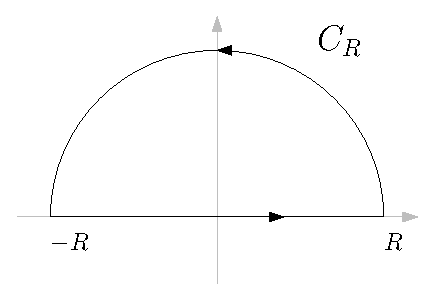
\includegraphics[scale=1]{circ.eps}
    \caption{Полукруг в верхней полуплоскости с обходом против часовой стрелки}
		\label{fig:13.1}
\end{figure}
\\
Пусть 
\begin{align*}
  & I_R = \int_{\gamma_R}f(z)dz = 2 \pi i \left( \us{z_0}{\res} f(z) +  \us{z_1}{\res} f(z)\right) = 2 \pi i \left( \left.\frac{1+z^2}{4z^3}\right|_{z_0} + \left.\frac{1+z^2}{4z^3}\right|_{z_1}\right) = 2 \pi i \cdot \\
  & \cdot \left( \frac{1+\exp\left( \frac{2i \pi}{4} \right)}{4 \exp \left( \frac{3i \pi}{4} \right)} +  \frac{1+\exp\left( \frac{6i \pi}{4} \right)}{4 \exp \left( \frac{9i \pi}{4} \right)}\right) = 2 \pi i \left( \frac{\exp\left( \frac{-i\pi}{4} \right) + \exp\left( \frac{i\pi}{4} \right)}{2 i \cdot 2} +  \frac{\exp\left( \frac{-3i\pi}{4} \right) + \exp\left( \frac{3i\pi}{4} \right)}{-2 i \cdot 2}\right) = \\
  & = \pi \left( \cos \frac{\pi}{4} - \cos \frac{3\pi}{4} \right) = \pi \sqrt{2}
\end{align*}
\begin{align*}
  & \pi \sqrt{2} = \int_{-R}^{+R}f(z) + \int_{C_R}f(z) \us{R\to \infty}{\longrightarrow} \int_{-\infty}^{+\infty} f(z) = \int_{-\infty}^{\infty}f(x)
\end{align*}
Итак, достаточно доказать
\begin{align*}
  & \int_{C_R}f(z)  \us{R\to \infty}{\longrightarrow} 0
\end{align*}
чтобы получить, что $I = \pi \sqrt{2}$.
    \begin{flushright}
    \textit{Лекция 10 (от 06.10)}
\end{flushright}
\Example
Вычисление несобственных интегралов.
\begin{equation}\label{(13.9)}
    I = \int_{-\infty}^{\infty}F_{n,m}(x)dx
\end{equation}
\begin{align*}
  & F_{n,m}(x) = \frac{P_n(x)}{Q_m(x)}, \ Q_m \neq 0 \ \forall x \in \RR, \ m > n+1
\end{align*}
Пусть $R_0 \in (0, R)$,$\gamma_r = [-R;R]\cap C_R$ (см. рис. \ref{fig:13.1}).
Пусть $z_k^+$~--- нули $Q_m(z)$, причем $\Img z_k^+ > 0, \ k \in \{1, \dots,
n\}$, $R_0 = \max \sets{z_k^+}$. Пусть
\begin{align*}
  & I_R = \int_{\gamma_R}F_{n,m}(z)dz = 2 \pi i \sum_{k=1}^n\us{z_k}{\res}F_{n,m}, \ R > R_0
\end{align*}
Но
\begin{align*}
  & I_R = \int_{C_R}F_{n,m}(z)dz + \int_{-R}^RF_{n,m}(z)dz
\end{align*}
Легко заметить, что
\begin{align*}
  & \lim_{R \to \infty} \int_{C_R}F_{n,m}(z)dz = 0
\end{align*}
Значит,
\begin{equation}\label{(13.10)}
    I = \int_{-\infty}^{\infty}F_{n,m}(x)dx = 2 \pi i \sum_{k=1}^n \us{z_k}{\res} F_{n,m}
\end{equation}
\lemma
Пусть $\Phi(z)$ непрерывна на $\sets{z \mid \Img z \geq 0, \abs{z} \geq R_0 >
  0}$.
\\
Пусть $\varepsilon(R) = \max \left\{ \left| \Phi(z) \right| : z \in C_R\right\},
\ R > R_0$. Пусть $\dst \lim_{R \to \infty}R\varepsilon(R) = 0$.
\\
Тогда
\begin{align*}
  & \lim_{R \to \infty }\int_{C_R}\Phi(z)dz = 0
\end{align*}
\pr
\begin{align*}
  & \left| \int_{C_R}\Phi(z)dz \right|\leq \int_{C_R}\left| \Phi(z) \right| dz \leq \varepsilon(R) \int_{C_R}dz = \pi R \varepsilon(R) \us{R \to \infty}{\to} 0
\end{align*}
Применив лемму, докажем равенство \eqref{(13.10)}.
\begin{align*}
  & F_{n,m}(z) = \frac{z^n(1+o(1))}{z^m(1+o(1))}
\end{align*}
\begin{align*}
  & \left| F_{n,m} \right| \leq 2 \left| z \right|^{n-m} \leq 2 R^{n-m}
\end{align*}
\begin{align*}
  & R\varepsilon(R) \leq 2R^{n-m+1} \us{R \to \infty}{\to} 0
\end{align*}
Таким образом доказали формулу \eqref{(13.10)}.
\Example
Вычисление несобственных интегралов.
\begin{equation}\label{(13.11)}
    I = \int_{-\infty}^{\infty}e^{i\alpha x}F_{n,m}(x)dx
\end{equation}
\begin{align*}
  & \alpha > 0, \ F_{n,m}(x) = \frac{P_n(x)}{Q_m(x)}, \ Q_m \neq 0 \ \forall x \in \RR, \ m > n
\end{align*}
Так же, как в предыдущем примере, задаем контур и $R$. По теореме Коши о вычетах
\begin{align*}
  & I_R = \int_{\gamma_R}e^{i\alpha z}F_{n,m}(z) dz = 2 \pi i \sum_{k=1}^n\us{z_k^+}{\res}\left( e^{i\alpha z} F_{n,m}(z)\right)
\end{align*}
Покажем, что
\begin{align*}
  & const = I_R = \int_{C_R}e^{i\alpha z}F_{n,m}(z) dz + \int_{-R}^Re^{i\alpha z}F_{n,m}(z) dz \us{R \to \infty}{\to} \int_{-\infty}^\infty e^{i\alpha z}F_{n,m}(z) dz
\end{align*}
то есть
\begin{equation}\label{(13.12)}
    \lim_{R \to \infty} \int_{C_R}e^{i\alpha z}F_{n,m}(z)dx = 0 \Rightarrow I = 2 \pi i \sum_{k=1}^n \us{z_k^+}{\res}\left( e^{i \alpha z}F_{n,m}(z) \right)
\end{equation}
\lemma (Жордана)
Пусть $\Phi(z)$ непрерывна на $\left\{ z \mid \left| z \right| \geq R_0, \Img z
    \geq 0 \right\}, \ R > R_0$, $C_R$~--- семейство полуокружностей $C_R = \{z
\mid \left| z \right| = R, \Img z \geq 0\}$, $ \varepsilon(R) = \max \left\{
    \left| \Phi(z) \right| : z \in C_R \right\}$, $ \dst \lim_{R \to \infty}
\varepsilon(R) = 0$, $\alpha > 0$. Тогда
\begin{equation}\label{(13.13)}
    \lim_{R \to \infty}\int_{C_R}e^{i \alpha z}\Phi(z)dz = 0
\end{equation}
\pr
$z = x + iy \in C_R$. Значит, положим $x = R \cos \varphi$, $y = R \sin \varphi$,
$ \varphi \in [0,\pi]$. Тогда
\begin{align*}
  & e^{i \alpha z} = e^{i \alpha(x+iy)} = e^{-\alpha y + i \alpha x} = e^{-\alpha R \sin \varphi + i \alpha R \cos \varphi}
\end{align*}
\begin{align*}
  & \left| e^{i \alpha z} \right| = e^{-\alpha R \sin \varphi}
\end{align*}
\begin{align*}
  & z = R e^{i \varphi} \Rightarrow dz = R i e^{i \varphi} d \varphi
\end{align*}
\begin{align*}
  & \left| \int_{C_R}e^{i \alpha z}\Phi(z) dz \right| \leq \int_{0}^{\pi}e^{-\alpha R \sin \varphi}\varepsilon(R) R d \varphi = \varepsilon(R) R \int_{0}^{\pi}e^{-\alpha R \sin \varphi}d \varphi = 2 \varepsilon(R) R \int_{0}^{\frac{\pi}{2}}e^{-\alpha R \sin \varphi}d \varphi \leq \\
  & \leq 2 \varepsilon(R) R \int_{0}^{\frac{\pi}{2}}\exp\left( -\alpha R \frac{2 \varphi}{\pi} \right) d \varphi = \frac{2 \varepsilon(R) R \pi}{2 \alpha R}\left( 1 - e^{-\alpha R} \right) \leq \frac{\pi}{\alpha} \varepsilon(R) \us{R \to \infty}{\to} 0
\end{align*}
Здесь использовали соотношение: $\forall \varphi \in \left[ 0, \dst
    \frac{\pi}{2} \right] \ \sin \varphi \geq \dst \frac{2 \varphi}{\pi}$.
\begin{align*}
  & z = R e^{i \varphi} \Rightarrow dz = R i e^{i \varphi} d \varphi
\end{align*}
Применив лемму, докажем равенство \eqref{(13.12)}. При достаточно больших по
модулю $z$ и $m-n \geq 1$
\begin{align*}
  & \left| F_{n,m}(z) \right| \leq 2 \left| z \right|^{n-m} \leq 2 R^{n-m} \leq \frac{2}{R} \us{R \to \infty}{\to} 0
\end{align*}
\begin{align*}
  & \int_{-\infty}^\infty e^{i \alpha x}F_{n,m}(x) dx = \int_{-\infty}^\infty \cos\alpha xF_{n,m}(x) dx + i \int_{-\infty}^\infty \sin \alpha x F_{n,m}(x) dx
\end{align*}
Таким образом доказали формулу \eqref{(13.12)}.
\section{$\S 14.$ Приращение аргумента $z$ вдоль кривой}
Как известно, $z = x + iy \neq 0 \Rightarrow \Arg z = \left\{\varphi + 2 \pi k
    \mid k \in \ZZ \right\}$. Значит,
\begin{equation}\label{(14.1)}
    \cos \varphi = \frac{x}{\left| z \right|}, \ \sin \varphi = \frac{y}{\left| z \right|}
\end{equation}
\theorem
Пусть $z: [0,1] \mapsto \CC$ непрерывно дифференцируема, $\forall t \in [0,1] \
z(t)\neq 0$. Пусть $\varphi_0 = \varphi(0) \in \Arg z(0)$. Тогда существует и
единственна функция $\varphi: [0,1] \mapsto \RR$, непрерывно дифференцируемая,
$\forall t \in [0,1] \ \varphi(t) \in \Arg z(t)$, т.~е.
\begin{equation}\label{(14.2)}
    \forall t \in [0,1] \ \cos \varphi(t) = \frac{x(t)}{\left| z(t) \right|}, \ \sin \varphi(t) = \frac{y(t)}{\left| z(t) \right|}
\end{equation}
и $\varphi(0) = \varphi_0$, причем $\varphi$ явно вычисляется как
\begin{equation}\label{(14.3)}
    \varphi(t) = \varphi_0 + \int_{0}^t \frac{x(\tau)y'(\tau)-y(\tau)x'(\tau)}{x^2(\tau)+y^2(\tau)}d \tau
\end{equation}
\pr
~
\begin{itemize}
    \item Существование.
    \\
    Рассмотрим \eqref{(14.3)} и покажем, что это решение \eqref{(14.2)}.
    Определим
    \begin{equation}\label{(14.4)}
        \left\{ \begin{matrix}
                u(t) = \cos \varphi(t) \\
                v(t) = \sin \varphi(t)
            \end{matrix} \right. \Rightarrow \left\{ \begin{matrix}
                u'(t) = \varphi'(t)\sin \varphi(t) = -v(t) \varphi'(t) \\
                v'(t) = \varphi'(t)\cos \varphi(t) = u(t) \varphi'(t) 
            \end{matrix} \right.
    \end{equation}
    Определим
    \begin{equation}\label{(14.5)}
        \begin{split}
            & \left\{ \begin{matrix}
                    \tilde{u}(t) = \dst \frac{x(t)}{\left| z(t) \right|} \\
                    \tilde{v}(t) = \dst \frac{y(t)}{\left| z(t) \right|} \\
                \end{matrix} \right. \Rightarrow \\
            & \left\{ \begin{matrix}
                    \dst \frac{d}{dt} \tilde{u}(t) = \dst \frac{d}{dt}\left( \dst \frac{x}{\sqrt{x^2+y^2}} \right) = \dst \frac{x'}{\left| z \right|} - \dst \frac{2x\left( xx'+yy' \right)}{\left| z \right|^3} = -\dst \frac{y}{\left| z \right|} \cdot \dst \frac{xy'-yx'}{x^2+y^2} = - \tilde{v} \dst \frac{xy'-yx'}{x^2+y^2} \\
                    \dst \frac{d}{dt} \tilde{v}(t) = \tilde{u} \dst \frac{xy'-yx'}{x^2+y^2} \\              
                \end{matrix} \right.
        \end{split}
    \end{equation}
    Из \eqref{(14.3)} заметим, что
    \begin{align*}
      \varphi'(t) = \frac{xy'-yx'}{x^2+y^2}
    \end{align*}
    Значит, \eqref{(14.4)} и \eqref{(14.5)} задают одинаковые дифференциальные
    уравнения. Поскольку $\varphi(0) = \varphi_0$ фиксировано. то $u(0) =
    \tilde{u}(0)$, $v(0) = \tilde{v}(0)$ и по теореме единственности $u(t) =
    \tilde{u}(t)$, $v(t) = \tilde{v}(t)$, откуда следует \eqref{(14.2)}.
    \item Единственность.
    \\
    Пусть $\exists \varphi_1(t) \in \Arg z(t)$, непрерывно дифференцируемая,
    $\varphi_1(0) = \varphi_0$ (это равносильно \eqref{(14.2)}); дифференцируя,
    из \eqref{(14.4)} и \eqref{(14.5)} получаем
    \begin{align*}
      \varphi_1'(t) = \frac{xy'-yx'}{x^2+y^2}
    \end{align*}
    а значит, эта функция находится по формуле \eqref{(14.3)} и совпадает с
    $\varphi$.
\end{itemize}
\note
Формулу \eqref{(14.3)} можем записать как
\begin{equation}\label{(14.6)}
    \varphi(t) = \varphi_0 + \Img \int_{0}^t \frac{z'(\tau)}{z(\tau)}d \tau
\end{equation}
\pr
\begin{align*}
  & \frac{z'}{z} = \frac{\left( x'+iy' \right)\left( x-iy \right)}{\left( x+iy \right)\left( x-iy \right)} = \frac{x'x+y'y+i\left( xy'-x'y \right)}{x^2+y^2}
\end{align*}
\begin{align*}
  & \Img \frac{z'}{z} = \Img \frac{x'x+y'y+i\left( xy'-x'y \right)}{x^2+y^2} = \frac{xy'-x'y}{x^2+y^2}
\end{align*}
\Def
\textbf{Приращением аргумента $z$ вдоль кривой $z(t)$} на отрезке $[0,1]$
называется
\begin{equation}\label{(14.7)}
    \Delta_{[0,1]}\argt z = \varphi(1) - \varphi(0) = \Img \int_{0}^1 \frac{z'(\tau)}{z(\tau)}d \tau
\end{equation}
\begin{figure}[h!]
		\centering
		\includegraphics[scale=0.8]{deltaarg.eps}
    \caption{Приращение аргумента вдоль кривой}
		\label{fig:14.1}
\end{figure}\\
\theorem (логарифмическое свойство)
Пусть $z(t) \in C^1[0;1]$, $\forall t \in [0,1] \ z(t) \neq 0$. Пусть $z(t) =
z_1(t)z_2(t)$, $z_k(t) \in C^1[0,1]$. Тогда
\begin{equation}\label{(14.8)}
    \Delta_{[0,1]}\argt z = \Delta_{[0,1]}\argt z_1 + \Delta_{[0,1]}\argt z_2
\end{equation}
\pr
Из \eqref{(14.7)} имеем:
\begin{align*}
  & \Delta_{[0,1]} \argt z(t) = \Img \int_{0}^{1}\frac{\left( z_1(\tau)z_2(\tau) \right)'}{z_1(\tau)z_2(\tau)}d \tau =\Img \int_{0}^{1}\frac{z_1'z_2+z_1z_2'}{z_1z_2}d \tau = \Img \int_{0}^{1}\frac{z_1'}{z_1}d \tau + \Img \int_{0}^{1}\frac{z_2'}{z_2}d \tau = \\
  & = \Delta_{[0,1]} \argt z_1(t) + \Delta_{[0,1]} \argt z_2(t) 
\end{align*}
\Def
Пусть $\gamma$~--- кривая в $\CC$, заданная параметризацией $z=z(t)$, $t \in
[0;1]$, $z \in C^1[0;1]$, $0 \not \in \gamma$. Тогда \textbf{приращением
  аргумента $z$ вдоль кривой $\gamma$} называется
\begin{equation}\label{(14.9)}
    \Delta_{\gamma}\argt z = \Delta_{[0;1]}\argt z = \Img \int_{0}^1 \frac{z'(\tau)}{z(\tau)}d \tau
\end{equation}
Определение корректно, т.~к. \eqref{(14.9)} равносильно
\begin{equation}\label{(14.10)}
    \Delta_{\gamma}\argt z = \Img \int_{\gamma} \frac{dz}{z}
\end{equation}
    \begin{Def}
	Векторным полем на $D$ называется функция $\vec{a}: D\to\R^n$.\\ $\vec{a}=a^1\vec{e_1}+\ldots+a^n\vec{e_n}$.
	Если $(\vec{e_1}, \ldots, \vec{e_n})$ --- ортонормированный базис евклидова пространства $\R^n$, то операции соответствия векторных полей и дифференциальных форм валентности $n$ определяются так: $(\vec{a})^\sharp=a_1(x)dx^1+\ldots+a_n(x)dx^n$ и для $\Omega(x)=w_1(x)dx^1+\ldots+w_n(x)dx^n$, $(\Omega)^\flat=w^1(x)\vec{e_1}+\ldots+w^n(x)\vec{e_n}$, где $a_i(x)=a^i(x), w_i(x)=w^i(x), i=1,\ldots, n, (dx^1, \ldots, dx^n)$ --- сопряженный базис к $(\vec{e_1}, \ldots, \vec{e_n})$.
	
	Аналогично определяются операции соответствия для поливекторных полей и дифференциальных форм произвольной валентности.
\end{Def}

\subsubsection{Основные операции теории поля.}
По сути все основные операции теории поля --- это дифференцирование дифференциальных форм.

Начнем с $0$-формы $f(x)$ в $\R^n:$
\begin{align*}
	df&=\dfrac{\partial f}{\partial x^1}dx^1+\ldots+\dfrac{\partial f}{\partial x^n}dx^n \\
	(df)^\flat&= \dfrac{\partial f}{\partial x^1}e_1+\ldots+\dfrac{\partial f}{\partial x^n}e_n=\grad f
\end{align*}

$1$-форма в $\R^3$:
$$
	(\vec{a})^\sharp= a_1(x)dx^1+a_2(x)dx^2+a_3dx^3=Pdx+Qdy+Rdz
$$
\begin{multline*}
	d(\vec{a})^\sharp=dP\wedge dx+dQ\wedge dy+dR\wedge dz=
	\\
	=\left(\dfrac{\partial P}{\partial x}dx+\dfrac{\partial P}{\partial y}dy+\dfrac{\partial P}{\partial z}dz \right)\wedge dx+\\+\left(\dfrac{\partial Q}{\partial x}dx+\dfrac{\partial Q}{\partial y}dy+\dfrac{\partial Q}{\partial z}dz \right)\wedge dy+\\+\left(\dfrac{\partial R}{\partial x}dx+\dfrac{\partial R}{\partial y}dy+\dfrac{\partial R}{\partial z}dz \right)\wedge dz=
	\\
	=\left(\dfrac{\partial R}{\partial y}-\dfrac{\partial Q}{\partial z}\right)dy\wedge dz+\left(\dfrac{\partial P}{\partial z}-\dfrac{\partial R}{\partial x}\right)dz\wedge dx+\left(\dfrac{\partial Q}{\partial x}-\dfrac{\partial P}{\partial y}\right)dx\wedge dy
\end{multline*}
$$*d(\vec{a})^\sharp = \left(\dfrac{\partial R}{\partial y}-\dfrac{\partial Q}{\partial z}\right)dx+\left(\dfrac{\partial P}{\partial z}-\dfrac{\partial R}{\partial x}\right)dy+\left(\dfrac{\partial Q}{\partial x}-\dfrac{\partial P}{\partial y}\right)dz$$
$$(*d(\vec{a})^\sharp)^\flat = \left(\dfrac{\partial R}{\partial y}-\dfrac{\partial Q}{\partial z}\right)\vec{i}+\left(\dfrac{\partial P}{\partial z}-\dfrac{\partial R}{\partial x}\right)\vec{j}+\left(\dfrac{\partial Q}{\partial x}-\dfrac{\partial P}{\partial y}\right)\vec{k}:=\rot\vec{a}$$

$(n-1)$-форма в $\R^n$:

$*(\vec{a})^\sharp=*(a_1(x)dx^1+\ldots+a_n(x)dx^n)=a_1(x)dx^2\wedge\ldots\wedge dx^n+\ldots+(-1)^{n-1}a_n(x)dx^1\wedge\ldots\wedge dx^{n-1}$.
\begin{multline*}
	d(*(\vec{a})^\sharp)=da_1(x)\wedge dx^2\wedge\ldots\wedge dx^n+\ldots+(-1)^{n-1}da_n(x)\wedge dx^1\wedge\ldots\wedge dx^{n-1}=\\=\dfrac{\partial a_1(x)}{\partial x^1}dx^1\wedge\ldots\wedge dx^n+\ldots+\dfrac{\partial a_n(x)}{\partial x^n}dx^1\wedge\ldots\wedge dx^n=\left(\dfrac{\partial a_1(x)}{\partial x^1}+\ldots + \dfrac{\partial a_n(x)}{\partial x^n}\right)dx^1\wedge\ldots\wedge dx^n.
\end{multline*}
$*d(*(\vec{a})^\sharp)=\dfrac{\partial a_1(x)}{\partial x^1}+\ldots+\dfrac{\partial a_n(x)}{\partial x^n}=\di\vec{a}$ --- дивергенция.

\begin{example}
	\begin{align*}
		\rot(\grad f)&=(*(d(\grad f)^\sharp))^\flat=(*(d(df)))^\flat=0\\
		\di(\rot\vec{a})&=*(d(*(\rot\vec{a})^\sharp))=*(d(**d(\vec{a}^\sharp)))=0
	\end{align*}
\end{example}

Векторный дифференциальный оператор набла: \fbox{$\nabla:=\left(\dfrac{\partial}{\partial x},\dfrac{\partial}{\partial y}, \dfrac{\partial}{\partial z}\right)$}.

\begin{align*}
	\grad f&= \left(\dfrac{\partial f}{\partial x}, \dfrac{\partial f}{\partial y}, \dfrac{\partial f}{\partial z}\right)=\nabla f\\
	\di\vec{a}&=\dfrac{\partial P}{\partial x}+\dfrac{\partial Q}{\partial y}+\dfrac{\partial R}{\partial z}=(\nabla, \vec{a})\\
	\rot\vec{a}&=[\nabla, \vec{a}]=
	\begin{vmatrix}
		\vec{i} & \vec{j} & \vec{k}\\
		\frac{\partial}{\partial x} & \frac{\partial}{\partial y} & \frac{\partial}{\partial z}\\
		P & Q & R
	\end{vmatrix}
\end{align*}


\begin{Def}
	$p$-форма $\Omega$ называется замкнутой, если $d\Omega=0$. $p$-форма $\Omega$ называется точной, если существует $(p-1)$-форма $\Pi$, такая что $\Omega=d\Pi$.
\end{Def}

\begin{corollary}
	Каждая точная форма замкнута. 
\end{corollary}

\begin{proof}
	Пусть $\Omega$ --- точная форма. Следовательно $\Omega=d\Pi\Rightarrow d\Omega=d(d\Pi)=0\Rightarrow\Omega$ --- замкнутая.
\end{proof}

\begin{Def}
	Область $D\subset\R^n$ называется звездной, если $\exists x_0\in D$, такое, что \\$ \varphi(x, t)=x_0+(1-t)(x-x_0)$, непрерывное отображение из $D\times[0,1]$ в $D$ и такое, что $\varphi(x,0)=x\ \ \forall x\in D, \varphi(x,1)=x_0\ \ \forall x\in D.$
	
	$\varphi$ --- называется прямым стягиванием $D$ в точку $x_0$.
\end{Def}

\subsubsection{Операция замены переменных в дифференциальной форме.}
\begin{Def}
	Пусть $\Omega(x)$ --- дифференциальная $p$-форма в области $U\subset\R^n, \varphi:V\to U$ --- диффеоморфизм области $V\subset\R^n$ на $U, x=\varphi(x).
	\\ \varphi^*\Omega(y)$ --- дифференциальная $p$-форма в области $V$, определяемая на любом наборе $p$ векторов из $\R^n, b_1,\ldots, b_p$, как  $\varphi^*\Omega(y)(b_1, \ldots, b_p)=\Omega(\varphi(y))(\varphi'(y)b_1, \ldots, \varphi'(y)b_p)$, где $\varphi'(y)$ --- это матрица Якоби отображения $\varphi$.
\end{Def} 

Пусть $\Omega(x)=w(x)dx^{i_1}\wedge\ldots\wedge dx^{i_p}$.

$(\varphi^*\Omega)(y)(b_1,\ldots, b_p)=w(\varphi(y))dx^{i_1}\wedge\ldots\wedge dx^{i_p}(\varphi'(y)b_1,\ldots, \varphi'(y)b_p)=w(\varphi(y))\det((\varphi'(y)b_j)^{i_k})_{j=1,k=1}^{p,p}$

Проверим, что $(\varphi^*\Omega)(y)=w(\varphi(y))d\varphi^{i_1}(y)\wedge\ldots\wedge d\varphi^{i_p}(y)$.

Подсчитаем 
\begin{multline*}
	w(\varphi(y))d\varphi^{i_1}(y)(b_1, \ldots, b_p)=w(\varphi(y))det(d\varphi^{i_k}(y)(b_j))_{j=1,k=1}^{p,p}=\\=w(\varphi(y))\det((\varphi'(y)d_j)^{i_k})_{j=1,k=1}^{p,p}\text{, так как }\\d\varphi^{i_k}(y)(b_j) = \sum\limits_{l=1}^n\dfrac{\partial \varphi^{i_k}}{\partial y^l}(y)(b_j^l)=(\varphi'(y)b_j)^{i_k}.
\end{multline*}

Правило подсчета $\varphi^*:$ если $\Omega(x)=\sum\limits_{1\leqslant i_1<\ldots<i_p\leqslant n}w_{i_1\ldots i_p}(x)dx^{i_1}\wedge\ldots\wedge dx^{i_p}$, то\\ 
$\varphi^*\Omega(y)=\sum\limits_{1\leqslant i_1<\ldots<i_p\leqslant n}w_{i_1\ldots i_p}(\varphi(y))d\varphi^{i_1}(y)\wedge\ldots\wedge d\varphi^{i_p}(y)$.
\subsubsection{Свойства операции замены переменных.}

\begin{enumerate}
	\item $\varphi^*(\alpha\Omega+\beta\Pi)=\alpha\varphi^*\Omega+\beta\varphi^*\Pi$
	\item
	$\varphi^*(\Omega\wedge\Pi)=\varphi^*(\Omega)\wedge\varphi^*(\Pi)$
	\item
	$\varphi^*(d\Omega)=d(\varphi^*\Omega)$
	\item 
	$\varphi^*\psi^*\Omega=(\varphi\psi)^*\Omega$
\end{enumerate}

\begin{proof}\ 
	\begin{enumerate}
		\item очевидно.
		\item\begin{multline*}
			\varphi(\Omega\wedge\Pi)=\\=\varphi^*\left(\sum\limits_{1\leqslant i_1<\ldots<i_p\leqslant n}\sum\limits_{1\leqslant j_1<\ldots<j_q\leqslant n}w_{i_1\ldots i_p}(x)\varpi_{j_1\ldots j_q}(x)dx^{i_1}\wedge\ldots\wedge dx^{i_p}\wedge dx^{j_1}\wedge\ldots\wedge dx^{j_q}\right)=\\=\sum\limits_{1\leqslant i_1<\ldots<i_p\leqslant n}\sum\limits_{1\leqslant j_1<\ldots<j_q\leqslant n}w_{i_1\ldots i_p}(\varphi(y))\varpi_{j_1\ldots j_q}(\varphi(y))d\varphi^{i_1}(y)\wedge\ldots\wedge d\varphi^{i_p}(y)\wedge \\ \wedge d\varphi^{j_1}(y)\wedge\ldots\wedge d\varphi^{j_q}(y)=\varphi^*(\Omega)\wedge \varphi^*(\Pi).
		\end{multline*} 
		\item 
		\begin{multline*}
			d\Omega(x)=\sum\limits_{1\leqslant i_1<\ldots<i_p\leqslant n}dw_{i_1\ldots i_p}(x)\wedge dx^{i_1}\wedge\ldots\wedge dx^{i^p}=
			\\
			=\sum\limits_{1\leqslant i_1<\ldots<i_p\leqslant n}\sum\limits_{k=1}^n\dfrac{\partial w_{i_1\ldots i_p}}{\partial x^k}(x)dx^{k}\wedge dx^{i_1}\wedge\ldots\wedge dx^{i_p}
		\end{multline*}
		$\varphi^*d\Omega(x)=\sum\limits_{1\leqslant i_1<\ldots<i_p\leqslant n}\sum\limits_{k=1}^n\dfrac{\partial w_{i_1\ldots i_p}}{\partial x^k}(\varphi(y))d\varphi^k(y)\wedge d\varphi^{i_1}(y)\wedge\ldots\wedge d\varphi^{i_p}(y)$
		
		$\varphi^*\Omega(y) = \sum\limits_{1\leqslant i_1<\ldots<i_p\leqslant n} w_{i_1\ldots i_p}(\varphi(y))d\varphi^{i_1}(y)\wedge\ldots\wedge d\varphi^{i_p}(y)$
		\begin{multline*}
			d\varphi^*\Omega(y)=\sum\limits_{1\leqslant i_1<\ldots<i_p\leqslant n}(dw_{i_1\ldots i_p}(\varphi(y))d\varphi^{i_1}(y)\wedge\ldots\wedge d\varphi^{i_p}(y)+\\+w_{i_1\ldots i_p}(\varphi(y))\underbrace{d(d\varphi^{i_1}(y)\wedge\ldots\wedge d\varphi^{i_p})}_{=0})
		\end{multline*}
	\item $\Omega=w(x)dx^{i_1}\wedge\ldots\wedge dx^{i_p}$ \\
	$\psi^*\Omega=w(\psi(y))d\psi^{i_1}(y)\wedge\ldots\wedge d\psi^{i_p}(y)$ \\
	$\varphi^*\psi^*\Omega=w(\psi(\varphi(z)))d\psi^{i_1}(\varphi(z))\wedge\ldots\wedge d\psi^{i_p}(\varphi(z))=(\varphi\psi)^*\Omega$
	\end{enumerate}
\end{proof}

\begin{Def}
	Область $G\subset\R^n$ называется звездообразной, если она является диффеоморфным образом звездной области.
\end{Def}

Если $\Omega$ --- дифференциальная форма в $D\times[0,1]$, то $\varphi^*\Omega$--- дифференциальная форма в $D$, где $\varphi$ --- прямое стягивание звездной области $D$, то $p$-форма $\Omega$ состоит из слагаемых вида $a(x,t)dx^{i_1}\wedge\ldots\wedge dx^{i_p}$ и $b(x,t)dt\wedge dx^{i_1}\wedge\ldots\wedge dx^{i_{p-1}}$.

$\Omega(x,t_0)$ при фиксированном $t_0$ будем считать дифференциальной формой на $D, dt\equiv 0$.

\begin{lemma}
	Если $\Omega$ --- гладкая $p$-форма в $D\times[0,1]$, то $(dK\Omega+Kd\Omega)(x)=\Omega(x,1)-\Omega(x,0)$, где $K$ --- линейная операция, заданная на базисных слагаемых как $K(a(x,t)dx^{i_1}\wedge\ldots\wedge dx^{i_p})=0,K(b(x,t)dt\wedge dx^{i_1}\wedge\ldots\wedge dx^{i_{p-1}})=\left(\int\limits_{0}^1b(x,t)d\mu(t)\right)\wedge dx^{i_1}\wedge\ldots\wedge dx^{i_{p-1}}$.
\end{lemma}

\begin{proof}\ 
	\begin{enumerate}
		\item На $a(x,t)dx^{i_1}\wedge\ldots\wedge dx^{i_{p}}: K\Omega=0, \\d\Omega=\dfrac{\partial a(x,t)}{\partial t}dt\wedge dx^{i_1}\wedge\ldots\wedge dx^{i_{p}}+\sum\limits_{k=1}^n\dfrac{\partial a(x,t)}{\partial x^k}dx^k\wedge dx^{i_1}\wedge\ldots\wedge dx^{i_{p}}$;\\ $Kd\Omega=\left(\int\limits_{0}^1\dfrac{\partial a(x,t)}{\partial t}d\mu(t)\right)dx^{i_1}\wedge\ldots\wedge dx^{i_p}=(a(x, 1)-a(x,0))dx^{i_1}\wedge\ldots\wedge dx^{i_p}\Rightarrow\\ (dK\Omega+kd\Omega)(x)=\Omega(x,1)-\Omega(x,0)$.
		\item При $b(x,t)dt\wedge dx^{i_1}\wedge\ldots\wedge dx^{i_{p-1}}=\Omega:\\ K\Omega=\left(\int\limits_{0}^1b(x,t)d\mu(x)\right)\wedge dx^{i_1}\wedge\ldots\wedge dx^{i_{p-1}}=\sum\limits_{k=1}^n \int\limits_{0}^1 \dfrac{\partial b(x,t)}{\partial x^k}d\mu(t)dx^k\wedge dx^{i_1}\wedge\ldots\wedge dx^{i_{p-1}}$
		$d\Omega=db(x,t)\wedge dt\wedge dx^{i_1}\wedge\ldots\wedge dx^{i_{p-1}}=\sum\limits_{k=1}^n\dfrac{\partial b(x,t)}{\partial x^k}dx^k\wedge dx^{i_1}\wedge\ldots\wedge dx^{i_{p-1}}=\\=-\sum\limits_{k=1}^n\dfrac{\partial b(x,t)}{\partial x^k}dt\wedge dx^k\wedge dx^{i_1}\wedge\ldots\wedge dx^{i_{p-1}}$\\
		$Kd\Omega=-\sum\limits_{k=1}^n\left(\int\limits_{0}^1 \dfrac{\partial b(x,t)}{\partial x^k}d\mu(t)\right)dx^k\wedge dx^{i_1}\wedge\ldots\wedge dx^{i_{p-1}}$\\
		$dK\Omega+Kd\Omega=0=\Omega(x,1)-\Omega(x,0)$
	\end{enumerate}
\end{proof}

\begin{theorem}(Лемма Пуанкаре)
	Каждая замкнутая в звездообразной области $D$ гладкая форма точна в ней.
\end{theorem}

\begin{proof}
	Пусть $D$ --- звездная область, $\varphi$ --- прямое стягивание. Рассмотрим $\varphi^*\Omega$ в $D\times[0,1]$. $\Omega$ --- замкнута $\Rightarrow d\Omega=0\Rightarrow d\varphi^*\Omega=\varphi^*d\Omega=0\Rightarrow \varphi^*\Omega$ --- замкнута в $D\times[0,1]$. Тогда по лемме $dK\varphi^*\Omega=-Kd\varphi^*\Omega+\varphi^*\Omega(x,1)-\varphi^*\Omega(x,0)$.
	
	$\Omega=\sum\limits_{1\leqslant i_1 < \ldots < i_p \leqslant n}w_{i_1\ldots i_p}(y)dy^{i_1}\wedge\ldots\wedge dy^{i_p}$, заменим переменную $y=\varphi(x,t)$,
	
	$\varphi^*\Omega=\sum\limits_{1\leqslant i_1 < \ldots < i_p \leqslant n} w_{i_1\ldots i_p}(\varphi(x,t))d\varphi^{i_1}(x,t)\wedge\ldots\wedge d\varphi^{i_p}(x,t)$,
	
	$d\varphi^{j}(x,t)=-(x^j-x_0^j)dt+(1-t)dx^j$. Считаем $dt\equiv0$, значит все слагаемые в которых появятся $dt$ обнулятся.
	
	$\varphi^*\Omega(x,1) =0$
	
	$\varphi^*\Omega(x,0)=\sum\limits_{1\leqslant i_1 < \ldots < i_p \leqslant n}w_{i_1\ldots i_p}(x)dx^{i_1}\wedge\ldots\wedge dx^{i_p}=\Omega(x)$. 
	
	Итого $dK\varphi^*\Omega=-\Omega(x)\Rightarrow \Omega(x)=d\Pi(x)$, где $\Pi(x)=-K\varphi^*\Omega$
	
	Пусть $D=\psi(G)$, где $G$ --- звездная область, $\psi$ --- диффеоморфизм. В $D$ есть замкнута форма $\Omega$. Рассмотрим $\psi^*\Omega$ --- форма в $G$, она замкнута, так как $d\psi^*\Omega=\psi^*d\Omega=0$. $G$ --- звездная область и по уже доказанному $\Pi=-K\varphi^*\psi^*\Omega$ является первообразной, то есть $d\Pi=\psi^*\Omega$. Тогда для $(\psi^{-1})^*\Pi$ справедливо $d(\psi^{-1})^*\Pi=(\psi^{-1})^*d\Pi=(\psi^{-1})^*\psi^*\Omega=\Omega$, в предположении, что $\varphi^*\psi^*\Omega=(\varphi\psi)^*\Omega$.
\end{proof}

\begin{Def}
	Векторное поле называется потенциальным, если оно является градиетном некоторой функции(скалярного поля), которое называется его потенциалом.
	
	$\vec{a}=\grad f, \vec{a}$ --- потенциальное поле, $f$ --- потенциал ($f+C$ --- тоже потенциал).
\end{Def}

\begin{Def}
	Векторное поле называется солениодальным, если оно является ротором некоторого векторного поля, которое называется векторным потенциалом исходного поля.
	
	$\vec{a}=\rot\vec{b}, \vec{a}$ --- соленоидальное поле, $\vec{b}$ --- векторный потенциал ($\vec{b}+\grad f$ --- тоже  векторный потенциал, так как $\rot\grad f=0$).
\end{Def}

\begin{corollary}[из определения]
	Если $\vec{a}$ --- потенциальное поле, то $\rot\vec{a}=\vec{0}$. Если $\vec{a}$ --- соленоидальное поле, то $\di\vec{a}=0$.
\end{corollary}

\begin{corollary}[из леммы Пуакаре]
	Если $\rot\vec{a}=0$ в звездообразной области $D$, то гладкое векторное поле $\vec{a}$ является потенциальным. Если $\di\vec{a}=0$ в звездообразной области $D$, то гладкое векторное поле $\vec{a}$ является соленоидальным.
\end{corollary}

\subsection{Интегрирование дифференциальных форм.}

Пространство $\Lambda_n(\R^n)$ одномерно. Если $(f^1,\ldots, f^n)$ --- базис $E^*$, то\\ $\{cf^1\wedge\ldots\wedge f^n:c\in\R^n\}=\Lambda_n(\R^n)$.

Пусть $(e_1^0,\ldots,e_n^0)$ --- ортонормированный базис $E$. $(e_1,\ldots, e_n)$ --- другой базис, $e_j=t^i_je_i^0$, $T$ --- матрица перехода.

$V_{e^0}:=dx^1_0\wedge\ldots\wedge dx^n_0$ --- базисный элемент пространства $n$-форм в любой точке области $D$.

$V_e:=dx^1\wedge\ldots\wedge dx^n$.

$V_{e^0}(e_1,\ldots, e_n)=dx^1_0\wedge\ldots\wedge dx^n_0(e_1,\ldots, e_n)=\det(dx_0^i(e_j))_{i=1,j=1}^{p,p}=\det T$.

$V_e(e_1,\ldots, e_n)=dx^1\wedge\ldots\wedge dx^n(e_1,\ldots, e_n)=1$.

\begin{prop}
	$V_{e^0}=\det TV_e$.
\end{prop}

\begin{Def}
	Два базиса называются эквивалентными, если $\det T>0$, где $T$ --- матрица перехода от одного базиса к другому.
\end{Def}

\begin{prop}
	Отношение эквивалентности базисов --- отношение эквивалентности на множестве базисов. Значит все базисы разбиваются на 2 класса эквивалентности. Задается ориентация базисов.
\end{prop}

Форма $V_e$ позволяет определить ориентацию базиса. Она назывется формой ориентированного объема.

Введем обозначение: $\Pi=\{0<x^i<1:i=1,\ldots,n\}$ --- призма, натянутая на векторы $e_1, \ldots, e_n$.

\begin{prop}
	$V_{e^0}=\pm \mu(\Pi)$, где $+$ соответствует положительно определенному относительно $(e_1^0,\ldots,e^0_n)$ базису $(e_1,\ldots, e_n)$.
\end{prop}




























    Дифференциальную форму валентности $n$ в $D\subset\R^n$ можно записать в виде $\Omega(x)=\alpha(x)V_{e^0}$, так как пространство полилинейных форм валентности $n$ в $n$-мерном пространстве одномерное.

\begin{Def}
	Интегралом от формы $\Omega(x)=\alpha(x)V_{e^0}$ по области $D\subset\R^n$ называется $\int\limits_{D}\Omega=\int\limits_{D}\alpha(x)d\mu(x)$, где $\alpha$ --- суммируемая на $D$.
\end{Def}

\begin{prop}
	Если $\varphi:G\to D$ --- гладкое отображение области $G\subset \R^n$ на $D$, такое, что $\det \varphi'(u)\ne 0\ \ \forall u\in G$ (то есть $\varphi$ --- неособое), то $\int\limits_{G}\varphi^*\Omega=\pm\int\limits_{D}\Omega$
\end{prop}

\begin{proof}
	\begin{multline*}
		\varphi^*\Omega(u)(H_1,\ldots, H_n)=\Omega(\varphi(u))(\varphi'(u)H_1, \ldots, \varphi'(u)H_n)=\\=\alpha(\varphi(u))V_{e^0}(\varphi'(u)H_1, \ldots, \varphi'(u)H_n)=\alpha(\varphi(u))dx_0^1\wedge\ldots\wedge dx^n_0(\varphi'(u)H_1, \ldots, \varphi'(u)H_n)=\\=\alpha(\varphi(u))\det((\varphi'(u)H_i)^j)=\alpha(\varphi(u))\det\varphi'(u)det(H^j_i)=\alpha(\varphi(u))\det\varphi'(u)\widetilde{V_{e^0}}(H_1,\ldots,H_n).
	\end{multline*}
	
	$\int\limits_{G}\varphi^*\Omega=\int\limits_{G}\alpha(\varphi(u))\det\varphi'(u)d\mu(u)$.
	
	$\int\limits_{D}\Omega=\int\limits_{D}\alpha(x)d\mu(x)=[x=\varphi(x)]=\int\limits_{G}\alpha(\varphi(u))|\det\varphi'(u)|d\mu(u)=\pm\int\limits_{G}\alpha(\varphi(u))\det\varphi'(u)d\mu(u)$
\end{proof}

\begin{Def}
	Стандартным кубом $K$ называется множество $\{0<x^i_0<1\},i=1,\ldots,n$ в ортонормированном базисе $e^0_1,\ldots,e_n^0$.
	
	Цепь стандартных кубов --- это линейная комбинация $\Pi=\sum\limits_{j=1}^mn_jK_j$, где $n_j\in \Z, K_j$ --- стандартные кубы.
\end{Def}

\begin{Def}
	Интеграл от $n$-формы $\Omega$ по цепи кубов определяется как $\int\limits_{\Pi}\Omega=\sum\limits_{j=1}^m n_j\int\limits_{K_j}\Omega$
\end{Def}

Граница стандартного куба --- цепь стандартных $(n-1)$-мерных кубов.

$\partial K=\sum\limits_{j=1, \alpha=0,1}^m\varepsilon_j^\alpha K_{j,\alpha},\ \ K_{j,\alpha}=\{0<x_0^i<1;i\ne j, x_0^j=\alpha\}$.

Правило ориентации граней куба: грань $K_{j,\alpha}$ ориентирована положительным базисом пространства $E_j=\{(x_0^1,\ldots,x_0^{j-1},x_0^{j+1},\ldots,x_0^n)\}$ таким, что дополнив его первым вектором, являющимся нормалью к грани $K_{j,\alpha}$, выходящей из куба $K$, получим положительный базис $\R^n$.













    \begin{flushright}
    \textit{Лекция 13 (от 19.10)}
\end{flushright}
\pr
Из леммы $5$ очевидно следует необходимость (возьмем $a = b$).
\\
Докажем достаточность. Пусть $a \in G$, $z \in G$, $\gamma_{az}\in G$, $g(a) \in
\left\{ \sqrt[n]{f(z)} \right\}$. Тогда выполняется
\begin{equation}\label{(16.16)}
    g(z) = g(a) \sqrt[n]{\left| \frac{f(b)}{f(a)} \right|}\exp \left( \frac{i}{n} \Delta_{\gamma_{az}}\arg f(z) \right)
\end{equation}
Докажем регулярность такой ветви.
\\
Для замкнутых кривых экспонента примет значение $1$, а значит, $g(z)$ зависит
только от точки $z$. Очевидно, $\forall z \in G \ g(z)\in \left\{ \sqrt[n]{f(z)}
\right\}$. Докажем ее регулярность.
\\
Фиксируем произвольную $z_1 \in G$; тогда $\exists B_\varepsilon(z_1) \subseteq G$
такой, что
\begin{equation}\label{(16.17)}
    \forall z \in B_\varepsilon(z_1) \ g(z) = g(z_1) \sqrt[n]{\left| \frac{f(z)}{f(z_1)} \right|}\exp \left( \frac{i}{n} \Delta_{\gamma_{z_1z}}\argt f(z) \right)
\end{equation}
$B_{\varepsilon}(z_1)$ односвязна, значит, по лемме $2$
$\Delta_{\os{\circ}{\gamma}}\argt f(z) = 0$ для любой замкнутой
$\os{\circ}{\gamma} \subseteq B_\varepsilon(z_1)$. Но
\begin{align*}
  & g(z) = \exp \left( \frac{i}{n} h(z) \right)
\end{align*}
\begin{align*}
  & h(z) = \ln \left| f(z) \right| + i \left(\psi_0 + \Delta_{\gamma_{z_1z}}\argt f(z)\right), \ \psi_0 \in \Arg f(z_1)
\end{align*}
\begin{equation}\label{(16.18)}
    g(z_1) = \sqrt[n]{\abs{f(z_1)}} \exp\left( \frac{i}{n}\psi_0 \right)
\end{equation}
В $B_\varepsilon(z_1)$ есть регулярная ветвь $\Ln f(z)$, причем $h(z)$~--- та
самая ветвь, значит, $g(z)$ регулярна в $B_\varepsilon(z_1)$.
\\
В силу произвольности выбора $z_1$ показали регулярность во всей $G$.
\corollary
Если $h(z)$, $g(z)$~--- регулярные ветви $\Ln f(z)$ и $\left\{ \sqrt[n]{f(z)}
\right\}$ соответственно в $G$, то
\begin{equation}\label{(16.19)}
    h'(z) = \frac{f'(z)}{f(z)}
\end{equation}
\begin{equation}\label{(16.20)}
    g'(z) = \frac{f'(z)}{n\left( g(z) \right)^{n-1}}
\end{equation}
\pr
\begin{align*}
  & e^{h(z)} \equiv f(z) \rightarrow h'(z)e^{h(z)} \equiv f'(z) \Rightarrow h'(z) \equiv \frac{f'(z)}{f(z)}
\end{align*}
\begin{align*}
  & (g(z))^n \equiv f(z) \Rightarrow n(g(z))^{n-1}g'(z) \equiv f'(z) \Rightarrow g'(z) = \frac{f'(z)}{n\left( g(z) \right)^{n-1}}
\end{align*}
\section{$\S 17.$ Примеры вычисления регулярных ветвей.}
\Example
\begin{align*}
  & \left\{ \sqrt[4]{z^3(z+1)} \right\}, \ G = \CC \setminus[-1;0]
\end{align*}
Если ветвь существует, то
\begin{align*}
  & g_1(2) = i \sqrt[4]{24}
\end{align*}
При этих условиях найти $g_1(i)$, $g'_1(i)$.
\nonum
Заметим: $f(z) = z^3(z+1)$, $n=4$. Видим, что в $G$ $f(z) \neq 0$.
\\
$\forall \os{\circ}{\gamma} \subseteq G$~--- замкнутой~--- рассмотрим
$\Delta_{\os{\circ}{\gamma}}\argt f(z)$.
\begin{align*}
  & \Delta_{\os{\circ}{\gamma}}\argt f(z) = \Delta_{\os{\circ}{\gamma}}\argt z^3(z+1) = 3 \Delta_{\os{\circ}{\gamma}}\argt z + \Delta_{\os{\circ}{\gamma}}\argt (z-1)
\end{align*}
\begin{figure}[h!]
		\centering
		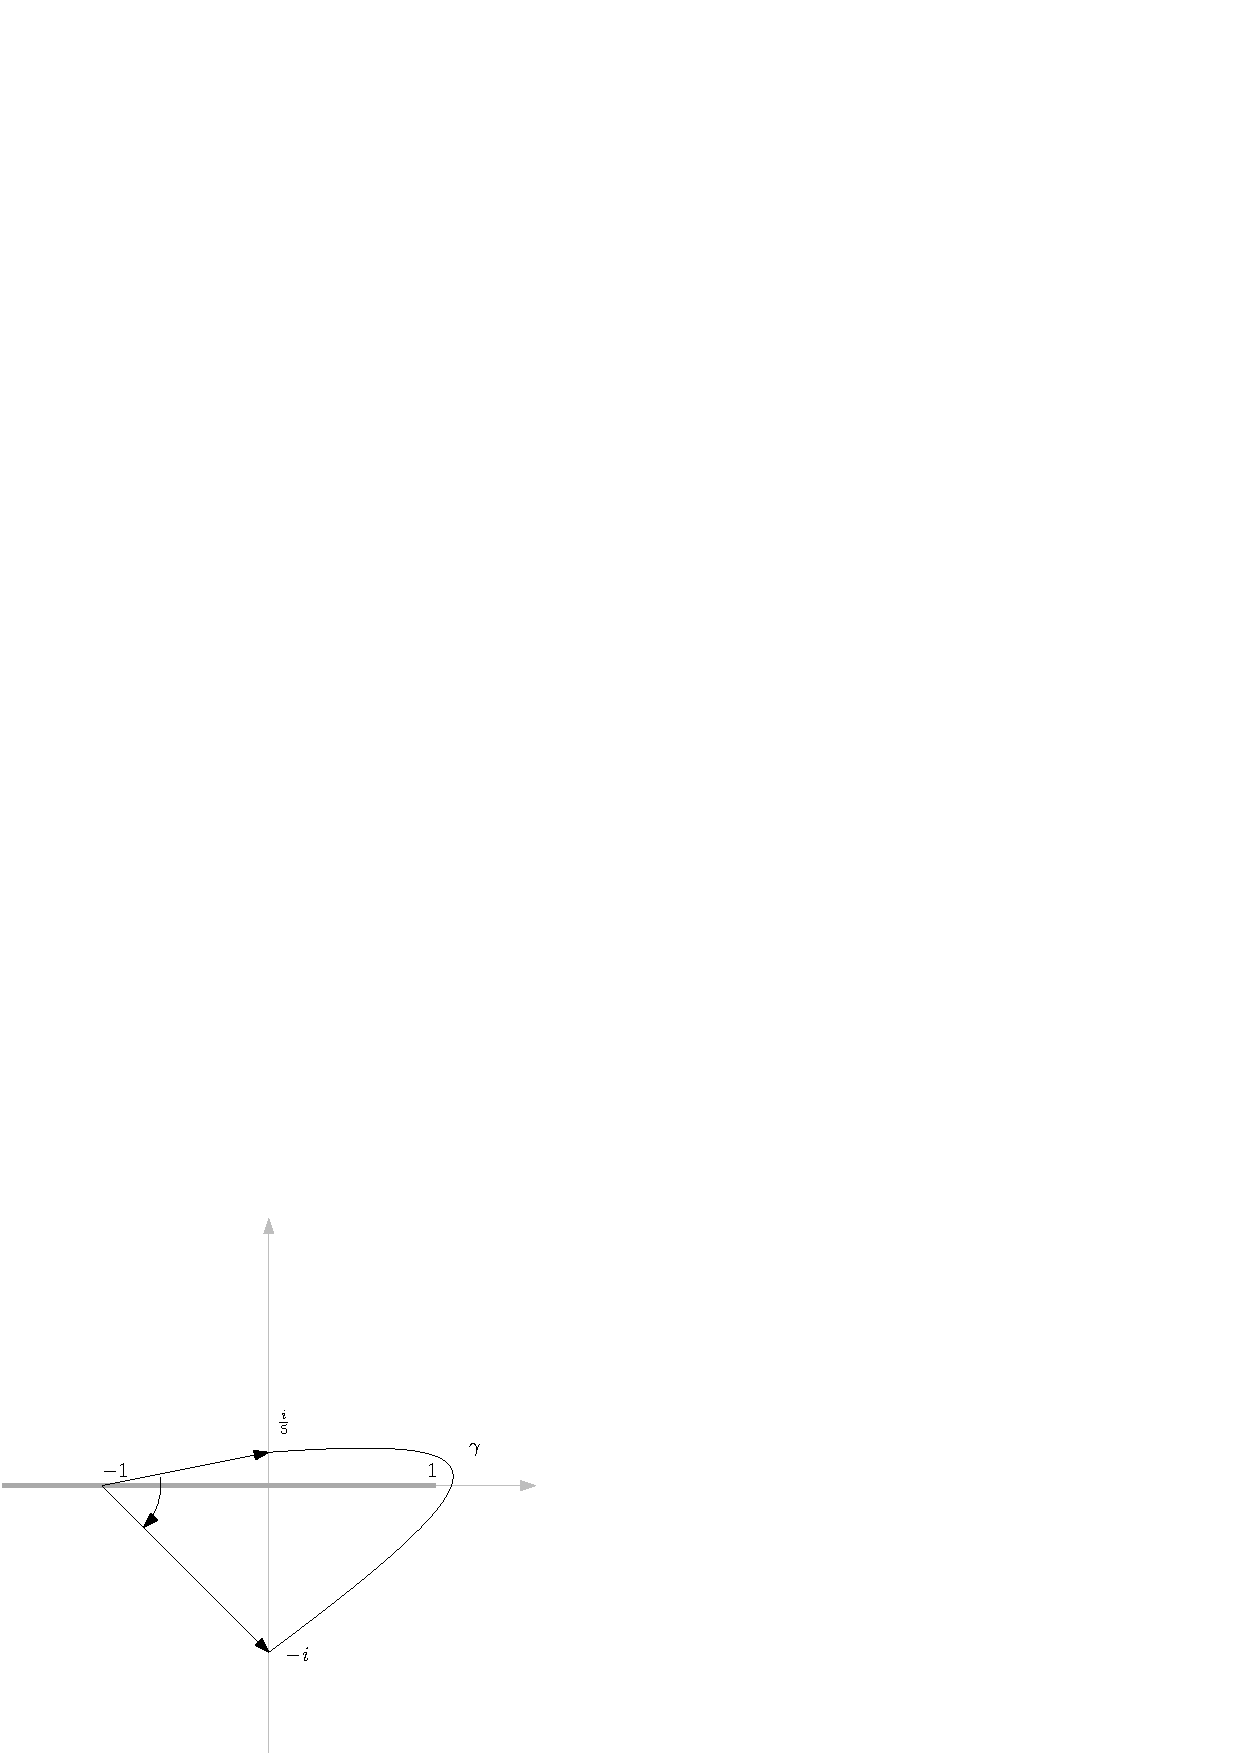
\includegraphics[scale=0.5]{Ex1.png}
		\label{fig:17.1}
\end{figure}
На кривых вида $\gamma_1$ (не опоясывающих разрез) приращение обоих аргументов
равно нулю (а значит, и суммарное), а на кривых вида $\gamma_2$ приращение
аргумента составит $8 \pi$. Оба случая удовлетворяют условию существования
регулярных ветвей.
\\
Докажем строго. Пусть $\os{\circ}{\gamma} = z(t)$, $t \in [0;1]$, $z(0) = z(1) =
z_0 \in \gamma$, $z(t, \alpha) = z(t) - \alpha$, $\alpha \in [-1;0]$. $\forall
(t, \alpha) \ z(t, \alpha) \neq 0$, $\forall \alpha \ z(1, \alpha) = z(0,
\alpha) = z_0 - \alpha$. Значит, по теореме $3$ $\S 14$ $I(\alpha) =
\Delta_{[0;1]}\argt z(t, \alpha) = const$, т.~е.
\begin{align*}
  & \Delta_{[0;1]} \argt z(t) = \Delta_{[0;1]} \argt(z(t) + 1) = \Delta_{\os{\circ}{\gamma}}z = \Delta_{\os{\circ}{\gamma}}(z+1) = 2 \pi k(\os{\circ}{\gamma})
\end{align*}
\begin{align*}
  & \Delta_{\ogamma} \argt f(z) = 4 \Delta_{\ogamma} \argt z = 8 \pi
\end{align*}
Желаемое условие выполняется.
\\
Значит,
\begin{align*}
  & g_1(z) = g_1(2) \sqrt[4]{\frac{\left| z^3(z+1) \right|}{24}} \exp \left( \frac{i}{4}\left( \Delta_{\gamma{2z}}\argt f(z) \right) \right)
\end{align*}
\begin{align*}
  & g_1(i) = g_1(2) \sqrt[4]{\frac{\left| i^3(i+1) \right|}{24}} \exp \left( \frac{i}{4}\left( \Delta_{\gamma_{2,i}}\argt f(z) \right) \right) = 2^{\frac{1}{8}}i\exp \left( \frac{i}{4} \left( 3\Delta_{\gamma_{2,i}}\argt z + \Delta_{\gamma_{2,i}} \argt (z+1) \right) \right) = \\
  & = 2^{\frac{1}{8}}i\exp \left( \frac{i}{4} \left( 3\frac{\pi}{2} + \frac{\pi}{4} \right) \right) = 2^{\frac{1}{8}}i\exp \left( \frac{7i\pi}{16} \right) =  2^{\frac{1}{8}}e^{\frac{15i\pi}{16}}
\end{align*}
\begin{align*}
  & g_1'(z) = \frac{4z^3+3z^2}{4g_1^3(z)}
\end{align*}
\begin{align*}
  & g_1'(i) = \frac{-4i -3}{4\cdot 2^{\frac{3}{8}}e^{\frac{45i\pi}{16}}} = -(4i+3)2^{-\frac{19}{8}}e^{-\frac{13i\pi}{16}}
\end{align*}
\Example
\begin{align*}
  & \Ln (1-z^2), \ G = \CC \setminus (-\infty; 1]
\end{align*}
Если ветвь существует, то
\begin{align*}
  & \Img h\left( \frac{i}{5} \right) = 0
\end{align*}
При этих условиях найти разложение $h$ в ряд Тейлора по степеням $(z+i)$,
область, где $h(z) = S(z)$~--- сумма своего ряда Тейлора, его радиус сходимости
$R$ и $S\left( \dst \frac{i}{5} \right)$.
\nonum
$G$ односвязна. Заметим: $f(z) = 1-z^2 \neq 0$ в $G$.
\\
$\forall \gamma \subseteq G$ рассмотрим $\Delta_{\gamma}\argt f(z)$.
\begin{align*}
  & h(z) = \ln \left| z \right| + i \Img h(z)
\end{align*}
\begin{align*}
  & h\left( \frac{i}{5} \right) = \ln \frac{26}{25}
\end{align*}
\begin{figure}[h!]
		\centering
		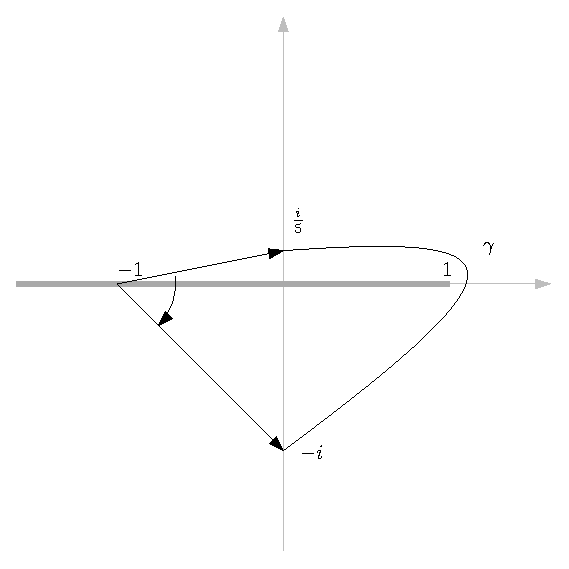
\includegraphics[scale=0.75]{Ex1.eps}
		\label{fig:17.2}
\end{figure}
\begin{align*}
  & h(-i) = \ln \frac{26}{25} + \ln \left| \frac{2}{\frac{26}{25}} \right|+ i\left( \Delta_{\gamma_{\frac{i}{5}, -i}}\argt (z+1) + \Delta_{\gamma_{\frac{i}{5}, -i}}\argt (z-1) + \Delta_{\gamma_{\frac{i}{5}, -i}}\argt (-1) \right) = \ln 2 - 2 i \pi
\end{align*}
Положим $\zeta = z+i$, $h(z) = h(\zeta - i) = \tilde{h}(\zeta)$. Тогда
$\tilde{h}(0) = h(-i) = \ln 2 - 2 i \pi$. Хотим разложить это в ряд.
\begin{align*}
  & \tilde{h}(\zeta) \in \Ln (1-(\zeta - i)^2) = \Ln(2+2i\zeta - \zeta^2) = \Ln \left(2\left( 1 - \frac{\zeta}{1-i} \right)\left( 1 - \frac{\zeta}{1+i} \right) \right) = \Ln 2 + \\
  & \Ln \left( 1 - \frac{\zeta}{1-i} \right) + \Ln \left( 1 - \frac{\zeta}{1+i} \right)
\end{align*}
Из теоремы об обратной функции
\begin{align*}
  & h^*_k(z) \in \Ln (1+z), \ \left| z \right| < 1 \Rightarrow h^*_k(z) = 2 i \pi k + \sum_{n=1}^\infty \frac{(-1)^{n+1}}{n} z^n, \ \left| z \right| < 1
\end{align*}
Рассмотрим
\begin{align*}
  & h_+(\zeta) \in \Ln \left( 1 - \frac{\zeta}{1+i} \right), \ \left| \zeta \right| < \sqrt{2}, \ h_+(0) = 0 \Rightarrow h_+(\zeta) = - \sum_{n=1}^\infty \frac{\zeta^n}{n(1+i)^n}, \ \left| \zeta \right| < \sqrt{2}
\end{align*}
\begin{align*}
  & h_-(\zeta) \in \Ln \left( 1 - \frac{\zeta}{1-i} \right), \ \left| \zeta \right| < \sqrt{2}, \ h_-(0) = 0 \Rightarrow h_-(\zeta) = - \sum_{n=1}^\infty \frac{\zeta^n}{n(1-i)^n}, \ \left| \zeta \right| < \sqrt{2}
\end{align*}
Заметим, что $\sqrt{2}$~--- максимальный радиус, т.~к. выходим на особую точку.
Видим:
\begin{align*}
  & \tilde{h}(\zeta) - h_+(\zeta) - h_-(\zeta) = \ln 2 + 2 i \pi k(\zeta)
\end{align*}
В правой части функция непрерывная, в левой ступенчатая, значит, $k = const$.
Найдем ее:
\begin{align*}
  &  \tilde{h}(0) - h_+(0) - h_-(0) = \ln 2 + 2 i \pi k = \ln 2 - 2 i \pi
\end{align*}
Значит, $k = -1$.
\\
Значит,
\begin{align*}
  & \tilde{h}(\zeta) = - \sum_{n=1}^\infty \frac{\zeta^n}{n(1+i)^n} - \sum_{n=1}^\infty \frac{\zeta^n}{n(1-i)^n} + \ln 2 - 2 i \pi
\end{align*}
\begin{align*}
  & h(z) = - \sum_{n=1}^\infty \frac{1}{n}\left( \frac{1}{(1+i)^n}+ \frac{1}{(1-i)^n}\right)(z-i)^n + \ln 2 - 2 i \pi, \ \left| z-i \right|< \sqrt{2}
\end{align*}
Видим, что $S(z)$ регулярна на $\left| z-i \right|< \sqrt{2}$; $S(z)$ и $h(z)$
есть регулярные ветви логарифма. Но также можем заметить, что часть разреза
лежит внутри круга сходимости. Тогда
\begin{align*}
  & \forall x \in (-1;1) \ h(x + i0) = h(x-i0) + i\Delta_{x+i0, x-i0}\argt h(z) = h(x-i0) + 2 i \pi \neq h(x-i0)
\end{align*}
Значит, внутри круга при положительной мнимой части $h(z) = S(z) + 2 i \pi$, а
при отрицательной мнимой части $h(z) = S(z)$.
\\
Значит,
\begin{align*}
  & S\left( \frac{i}{5} \right) = \ln \frac{25}{26} - 2 i \pi
\end{align*}
\begin{align*}
  & S'\left( \frac{i}{5} \right) = \left. \frac{-2z}{(1-z^2)} \right|_{z=\frac{i}{5}} = \frac{-2i\cdot 25}{5\cdot 26} = -\frac{5i}{13}
\end{align*}
\Def
Пусть $a, b \in \CC$, $a \neq 0$. Тогда
\begin{equation}\label{(17.1)}
    \left\{ a^b \right\} = \exp\left( b \Ln a\right)
\end{equation}
\Exse
Если $b = n$ или $b = \dst \frac{1}{n}$, $n\in \NN$, то \eqref{(17.1)} описывает
$a^n$ или $\left\{ \sqrt[n]{a} \right\}$ соответственно.
\Example
Разложить в ряд Тейлора регулярные ветви функции
\begin{align*}
  & \left\{ (1+z)^b \right\}, \ \left| z \right|<1
\end{align*}
\nonum
По определению,
\begin{align*}
  & (1+z)^b = \exp \left( b \Ln (1+z) \right)
\end{align*}
В силу существования регулярных ветвей у логарифма в этом круге ($h_k(0) = 2 i
\pi k$, $h_k$~--- регулярные ветви), то есть и регулярные ветви данной функции
будут существовать и иметь вид $w_k(z) = \exp \left( b h_k(z) \right)$.
\Exse
Доказать, что любая регулярная ветвь этой функции имеет такой вид.
\\
Вычислим производные $w_k$.
\begin{align*}
  & w_k(0) = e^{2bi\pi k}
\end{align*}
\begin{align*}
  & w_k'(z) = w_k(z) \frac{b}{1+z} \Rightarrow w_k'(0) = be^{2bi\pi k}
\end{align*}
\begin{align*}
  & w_k''(z) = w_k(z) \frac{b(b-1)}{(1+z)^2} \Rightarrow w_k''(0) = b(b-1)e^{2bi\pi k}
\end{align*}
\begin{align*}
  & w_k^{(n)}(z) = w_k(z) \frac{b(b-1)\dots(b-n+1)}{(1+z)^n} \Rightarrow w_k^{(n)}(0) = b(b-1)\dots(b-n+1)e^{2bi\pi k}
\end{align*}
\begin{align*}
  & w_k(z) = w_k(0)\sum_{n=0}^\infty C_b^nz^n
\end{align*}
\Example
Разложить в ряд Тейлора функцию
\begin{align*}
  & g \in \left\{ \sqrt[3]{1-z^2} \right\}, \ B_1(0), \ g(0) = \exp \left( \frac{2 i \pi}{3} \right)
\end{align*}
\nonum
По аналогии с предыдущим примером,
\begin{align*}
  & g(z) = \exp \left( \frac{2 i \pi}{3}\sum_{n=1}^\infty C_{\frac{1}{3}}^n(-1)^n z^{2n} \right)
\end{align*}
\Example
Разложить в $\os{\circ}{B}_1(\infty)$ в ряд Лорана регулярные ветви функции
\begin{align*}
  & \sets{\sqrt[4]{z^3(z+1)}}
\end{align*}
\nonum
\begin{align*}
  & \os{\circ}{B}_1(\infty) = \left\{ z \mid \left| z \right| > 1\right\}\subseteq \CC \setminus [-1;1]
\end{align*}
По аналогии с примером $1$
\begin{align*}
  & g_k(z) = \sqrt[4]{24}\exp \left( \frac{i\pi k}{2} \right)
\end{align*}
При $x > 2$, $x \in \RR$
\begin{align*}
  & g_0(x) = \sqrt[4]{x^3(x+1)} = x \sqrt[4]{1+\frac{1}{x}} = x \sum_{n=1}^\infty C_{\frac{1}{4}}^n\left( \frac{1}{x} \right)^n = S(x)
\end{align*}
\begin{align*}
  & \forall x \in \RR \cap (2; \infty) \ g_0(x) = S(x)
\end{align*}
Обе функции $S(z)$ и $g_0(z)$ регулярны, и по теореме единственности $g_0(z) =
S(z)$, а значит, искомый ряд Лорана будет иметь вид
\begin{align*}
  & z \sum_{n=1}^\infty C_{\frac{1}{4}}^n\left( \frac{1}{z} \right)^n
\end{align*}

    \begin{flushright}
    \textit{Лекция 14 (от 20.10)}
\end{flushright}
\section{$\S 18.$ Вычисление интегралов от регулярных ветвей.}
\Example
Вычислить при помощи теории вычетов интеграл
\begin{align*}
  & I = \int_0^2 \frac{\sqrt[4]{x^3(2-x)}}{(1+x)^2} dx
\end{align*}
\nonum
$g(z) = \sqrt[4]{z^3(2-z)}$ дает многозначную функцию. Отыщем регулярные ветви;
рассмотрим область, где ветви существуют. Функция $f(z) = z^3(2-z)$ должна быть
в области регулярной и не равной нулю.
\\
Рассмотрим $\CC \setminus [0;2]$. В такой области этот корень имеет регулярную
ветвь.
\\
Отыщем ветвь, что нам нужна. Построим ее так, чтобы $g(1+i0) = 1$; тогда
$\forall x \in [0;2] \ g(x+i0) = \sqrt[4]{x^3(2-x)}$. В этом случае
\begin{align*}
  & g(x-i0) = g(1+i0)\sqrt[4]{\frac{\left| g(x-i0) \right|}{\left| g(1+i0) \right|}}\exp\left( \frac{i}{4}\left( 3\Delta_{\gamma_{1+i0,x}}\argt z + \Delta_{\gamma_{1+i0,x}}\argt (2-z) \right) \right) = \\
  & = \sqrt[4]{\frac{\left| g(x-i0) \right|}{\left| g(1+i0) \right|}}\exp\left( \frac{-i\pi}{2}\right)
\end{align*}
\begin{figure}[h!]
		\centering
		\includegraphics[scale=0.75]{Par18.eps}
		\label{fig:18.1}
\end{figure}
Рассмотрим
\begin{align*}
  & \gamma_\varepsilon = I_\varepsilon^+\cup C_{2, \varepsilon} \cup I_\varepsilon^-\cup C_{0, \varepsilon}
\end{align*}
и
\begin{align*}
  & F(z) = \frac{\sqrt[4]{z^3(2-z)}}{(1+z)^2} = \frac{g(z)}{(1+z)^2}
\end{align*}
и вычислим
\begin{align*}
  & I_\varepsilon = \int_{\gamma_\varepsilon}F(z) dz = 2 i \pi \left( \us{-1}{\res} F(z) + \us{\infty}{\res} F(z) \right)
\end{align*}
Видим, что $-1$~--- полюс $2$ порядка, а $\infty$~--- УОТ.
\begin{align*}
  & \us{-1}{\res} F(z) = \lim_{z \to -1}((z+1)^2F(z))' = \lim_{z \to -1}g'(z) = g'(-1) = \left. \frac{f'(z)}{4g^3(z)}\right|_{z = -1} = \frac{-4(-1)^3+6(-1)^2}{4\left( \sqrt[4]{3}\exp\left( \frac{3i\pi}{4} \right)\right)^3} = \\
  & = \frac{5}{2\sqrt[4]{27}}\exp\left( \frac{-i\pi}{4} \right)
\end{align*}
Рассмотрим $x \in (2; \infty)$; тогда
\begin{align*}
  & g(x) = \sqrt[4]{x^3(2-x)}\exp\left( \frac{-i\pi}{4} \right) = x\sqrt[4]{1-\frac{2}{x}}\exp \left( \frac{-i\pi}{4} \right) = x\exp\left( \frac{-i\pi}{4} \right)\sum_{n=0}^\infty C_{\frac{1}{4}}^n\left( -\frac{2}{x} \right)^n
\end{align*}
Две регулярные функции ($g(x)$ и сумма) совпадают на $(2; \infty)$, а значит, по
теореме единственности
\begin{align*}
  & g(z) = z\exp\left( \frac{-i\pi}{4} \right)\sum_{n=0}^\infty C_{\frac{1}{4}}^n\left( -\frac{2}{z} \right)^n, \ \left| z \right|> 2
\end{align*}
\begin{align*}
  & F(z) = \frac{z}{(z+1)^2}h(z), \ h(z) = \exp\left( \frac{-i\pi}{4} \right)\sum_{n=0}^\infty C_{\frac{1}{4}}^n\left( -\frac{2}{z} \right)^n
\end{align*}
Заметим, что
\begin{align*}
  & \frac{z}{(1+z)^2} = \frac{1}{z(1+\frac{1}{z})^2} = \frac{1}{z} \left( 1-\frac{2}{z} +\frac{3}{z^2} + \dots \right)
\end{align*}
При перемножении двух рядов получим
\begin{align*}
  & \us{\infty}{\res}F(z) = -\exp\left( \frac{-i\pi}{4} \right)
\end{align*}
и интеграл
\begin{align*}
  & I_\varepsilon = 2 i \pi \left( \frac{5}{2\sqrt[4]{27}} - 1 \right)\exp\left( \frac{-i\pi}{4} \right)
\end{align*}
не зависит от $\varepsilon$. Заметим, что
\begin{align*}
  & I_\varepsilon = \int_{I_\varepsilon^+}F(z) + \int_{C_{2, \varepsilon}}F(z) + \int_{I_\varepsilon^-}F(z) + \int_{C_{0, \varepsilon}}F(z)
\end{align*}
Причем
\begin{align*}
  & \int_{I_\varepsilon^+}F(z) = \int_{\varepsilon}^{2-\varepsilon}\frac{\sqrt[4]{x^3(2-x)}}{(x+1)^2}dx
\end{align*}
\begin{align*}
  & \int_{I_\varepsilon^-}F(z) = \int_{2-\varepsilon}^{\varepsilon}\frac{g(x-i0)}{(x+1)^2}dx = -\int_{\varepsilon}^{2-\varepsilon}\frac{\sqrt[4]{x^3(2-x)}\exp\left( \frac{3i\pi}{2} \right)}{(x+1)^2}dx = -\exp\left( \frac{3i\pi}{2}\right) \int_{I_\varepsilon^+}F(z)
\end{align*}
Учтя $z = \varepsilon e^{i \varphi}$,
\begin{align*}
  & \left|  \int_{C_{0, \varepsilon}}F(z) \right| \leq \int_{0}^{2 \pi}\frac{\varepsilon\sqrt[4]{\varepsilon^3(2+\varepsilon)}}{(1-\varepsilon)^2}d\varphi \leq A\varepsilon^{\frac{7}{3}} \us{\varepsilon \to 0}{\to} 0
\end{align*}
Учтя $z = 2 + \varepsilon e^{i \varphi}$,
\begin{align*}
  & \left|  \int_{C_{2, \varepsilon}}F(z) \right| \leq \int_{0}^{2 \pi}\frac{\varepsilon\sqrt[4]{(2+\varepsilon)^3\varepsilon}}{(3-\varepsilon)^2}d\varphi \leq B\varepsilon^{\frac{4}{3}} \us{\varepsilon \to 0}{\to} 0
\end{align*}
Значит,
\begin{align*}
  & 2 i \pi \left( \frac{5}{2\sqrt[4]{27}} - 1 \right)\exp\left( \frac{-i\pi}{4} \right) = I_\varepsilon \us{\varepsilon \to 0}{\to} \int_{I_\varepsilon^+}F(z) + \int_{I_\varepsilon^-}F(z) = \left( 1 -\exp\left( \frac{3i\pi}{2}\right) \right) \int_{I_\varepsilon^+}F(z) \us{\varepsilon \to 0}{\to} \\
  & \us{\varepsilon \to 0}{\to} \left( 1 -\exp\left( \frac{3i\pi}{2}\right) \right) I
\end{align*}
Значит,
\begin{align*}
  & I = \frac{2 i \pi \left( \dst \frac{5}{2\sqrt[4]{27}} - 1 \right)\exp\left( \dst\frac{-i\pi}{4} \right)}{\left( 1 -\exp\left( \dst \frac{3i\pi}{2}\right) \right)}= \pi \sqrt{2}\left( \dst \frac{5}{2\sqrt[4]{27}} - 1 \right)
\end{align*}
\section{$\S 19.$ Целые и мероморфные функции.}
\Def
Функция $f$ называется \textbf{целой}, если она регулярна на $\CC$.
\\
Можем представить такую функцию в виде
\begin{equation}\label{(19.1)}
    \forall z \in \CC \ f(z) = \sum_{n=0}^\infty c_nz^n, \ c_n = \frac{1}{2i\pi}\int_{\gamma_r}\frac{f(\zeta)}{\zeta^{n+1}} d \zeta
\end{equation}
\theorem
Пусть $f:G \mapsto \CC$ целая, $\exists A > 0, \ R > 0, \ m \in \NN_0$ такие,
что $\forall z: \left| z \right| > R \hookrightarrow \left| f(z) \right| \leq
A\left| z \right|^m$. Тогда $f(z)$~--- многочлен степени $\leq m$.
\pr
Воспользуемся оценкой $c_n$.
\begin{align*}
  & \forall r > R \ \left|c_n \right| \leq \frac{1}{2\pi}\int_{\left| \zeta \right| = r} \frac{\left| f(\zeta) \right|}{\left| \zeta \right|^{n+1}}\left| d\zeta \right|\leq \frac{1}{2\pi}\frac{Ar^m}{r^{n+1}}r\cdot 2 \pi = Ar^{m-n}
\end{align*}
Значит, $\forall n > m \ c_n = 0$.
\corollary (теорема Лиувилля)
Если $f$ целая, $\exists R > 0, \ A > 0$: $\left| f(z) \right|< A$ при $\left| z
\right| > R$, то $f \equiv const$.
\theorem (Основная теорема алгебры)
Всякий многочлен $P_n(z) = z^n + C_{n-1}z^{n-1}+\dots+c_0$ имеет в $\CC$ хотя бы
один корень.
\pr
предположим, $\forall z \in \CC \ P_n(z) \neq 0$. Тогда $\varphi(z) = \dst
\frac{1}{P_n(z)}$ целая. Но, как легко видеть,
\begin{align*}
  & \lim_{z \to \infty}P_n(z) = \infty \Rightarrow \lim_{z \to \infty} \varphi(z) = 0 \Rightarrow \exists R > 0: \ \forall z: \ \left| z \right| > R \hookrightarrow \left| \varphi(z) \right| < 1
\end{align*}
Значит, по теореме Лиувилля $\varphi(z) = const$, тогда и $P_n(z) = const$.
Противоречие.
\\
Значит, можем заметить, что для целой функции $f$ единственная особая точка~---
это $\infty$.
\begin{itemize}
    \item $\infty$~--- УОТ, тогда $f = const$.
    \item $\infty$~--- полюс порядка $m$, тогда $f = P_m$.
    \item $\infty$~--- СОТ.
\end{itemize}
\Def
Целая функция, у которой $\infty$ есть СОТ, назвается \textbf{целой
  трансцендентной}.
\theorem (Сохоцкого)
Пусть $f$~--- целая трансцендентная функция, тогда
\begin{align*}
  & \forall A \in \CCC \ \exists z_n \to \infty: \ \lim_{n \to \infty}f(z_n) = A
\end{align*}
\pr
Рассмотрим два случая.
\begin{itemize}
    \item $A = \infty$
    \\
    $f$ неограничена в окрестности $\infty$ (т.~к. иначе она бы имела конечный
    предел), т.~е.
    \begin{align*}
      & \forall n \in \NN \ \exists z_n \in \CC: \left| f(z_n) \right|> n, \ \left| z_n \right| > n
    \end{align*}
    Итак, $\left\{ z_n \right\}$ и есть та самая последовательность.
    \item $A \in \CC$
    \\
    Пусть, от противного,
    \begin{align*}
      & \exists \delta_0 > 0, \ \varepsilon_0 > 0: \ \forall z: \ \left| z \right| \geq \delta_0 \ \left| f(z) - A \right| \geq \varepsilon_0
    \end{align*}
    Пусть $\varphi(z) = \dst \frac{1}{f(z) - A}$, $z \in B_{\delta_0}(\infty)$.
    На этом множестве
    \begin{align*}
      & \left| \varphi(z) \right| \leq \frac{1}{\varepsilon_0}
    \end{align*}
    Значит, эта функция на этом множестве регулярна и ограничена, а значит, для
    нее $\infty$~--- УОТ, т.~е.
    \begin{align*}
      & \exists \lim_{z \to \infty}\varphi(z) = B
    \end{align*}
    Значит, $\infty$~--- полюс либо УОТ для $f(z)$, противоречие.
\end{itemize}
\theorem (общая теорема Сохоцкого)
Пусть $f: \os{\circ}{B}_r(a) \mapsto \CC$ регулярна, $a$~--- СОТ $f$. Тогда
\begin{align*}
  & \forall A \in \CCC \ \exists z_n \to a, \ \lim_{n \to \infty} f(z_n) = A
\end{align*}
\Exse
доказать общую теорему Сохоцкого.
\theorem (Пикара)
Пусть $f$~--- целая трансцедентная функция, тогда $\forall a \in \CC$, за
исключением, быть может, одного, $\exists R > 0$: в $\os{\circ}{B}_R(\infty)$
существует бесконечное число решений уравнения $f(z) = A$, т.~е.
\begin{align*}
  & \exists z_n \to \infty: \ \forall n \in \NN \ f(z_n) = A
\end{align*}
\Example
$e^z = A$ имеет счетное число решений в любой окрестности бесконечности при $A
\neq 0$, но ни одного решения при $A = 0$.
\Exse
Пусть $f$~--- целая функция и
\begin{align*}
  & \exists A > 0, R > 0, \ m \in \NN_0: \ \forall z: \ \left| z \right| > R \ \left| f(z) \right| \geq A \left| z \right|^m
\end{align*}
Доказать, что $f$~--- многочлен степени $\leq m$.
\Def
Функция $f$ называется мероморфной, если $\forall R > 0$ в круге $B_R(0)$ она
регулярна за исключением, быть может, конечного числа полюсов.
\Example
\begin{align*}
  & f(z) = \frac{P_n(z)}{Q_m(z)}
\end{align*}
Конечное число полюсов на всей $\CC$.
\Example
\begin{align*}
  & f(z) = \ctg z
\end{align*}
Счетное число полюсов на $\CC$.
\Example
\begin{align*}
  & f(z) = \frac{z}{e^z-1}
\end{align*}
Счетное число полюсов на $\CC$.
    \begin{flushright}
    \textit{Лекция 15 (от 26.10)}
\end{flushright}
$f$ мероморфна~--- тогда существует $\left\{ z_k \right\}_{n=1}^{\infty}$~---
полюсы $m_k$ порядков.
\\
Тогда $\exists \os{\circ}{B}_{\delta_k}(z_k)$, где ряд Лорана
\begin{equation}\label{(19.2)}
    f(z) = \frac{c^k_{-m_k}}{(z-z_k)^{m_k}} + \dots + \frac{c^k_{-1}}{z-z_k} + c_0^k= c_1^k(z-z_k) + \dots
\end{equation}
а его главная часть
\begin{equation}\label{(19.3)}
    q_k(z) = \frac{c^k_{-m_k}}{(z-z_k)^{m_k}} + \dots + \frac{c^k_{-1}}{z-z_k}
\end{equation}
\theorem
Пусть $f$ мероморфна, $\infty$~--- УОТ или полюс этой функции. Тогда $f$
рациональна.
\pr
$\left\{ z_k \right\}$~--- полюсы $m_k$ порядка. В силу изолированности $\infty$
набор полюсов конечен; пусть $k \in \left\{ 1, \dots, l \right\}$.
\\
$\infty$~--- УОТ или полюс; главная часть ряда Лорана в окрестности $\infty$
будет иметь вид
\begin{align*}
  & q_0 = c_1z+\dots +c_nz^n
\end{align*}
Из \eqref{(19.3)} получим $q_k(z)$ для любого $k$.
\\
Тогда
\begin{equation}\label{(19.4)}
    r(z) = f(z) - \sum_{k=0}^lq_k(z)
\end{equation}
Заметим, что $\forall k$ $r(z)$ имеет в $z_k$ устранимую особую точку. Эта
функция, доопределенная по непрерывности, будет регулярной в $\CC$ и
ограниченной на бесконечности, а значит, по теореме Лиувилля $r(z) \equiv a_0$.
Тогда из \eqref{(19.4)} получим
\begin{align*}
  & f(z) = a_0 + \sum_{k=0}^lq_k(z)
\end{align*}
а значит, $f$ рациональна.
\Def
Совокупность замкнутых простых кусочно гладких кривых $\left\{ \Gamma_n
\right\}_{n=1}^\infty$ называется \textbf{правильной}, если
\begin{itemize}
    \item $\forall n \in \NN$ область $D_n$, ограниченная $\Gamma_n$, содержится
    в области $D_{n+1}$, ограниченной $\Gamma_{n+1}$, причем $0 \in D_1$;
    \item $d_n = \min \left\{ \left| z \right| : z \in \Gamma_n \right\}
    \Rightarrow \dst \lim_{n \to \infty}d_n = \infty$;
    \item $\exists A > 0: \ \forall n \in \NN \ l_n \leq Ad_n$, где $l_n  =
    l(\Gamma_n)$.
\end{itemize}
\example
Вложенные окружности, вложенные квадраты с центром в точке $0$.
\theorem (Коши)
Пусть $f$ мероморфна и существует правильная совокупность $\left\{ \Gamma_n
\right\}_{n=1}^\infty$, такая, что:
\begin{itemize}
    \item $\varepsilon_n = \max\left\{ \left| f(z) \right|: z \in \Gamma_n
    \right\}: \ \dst \lim_{n \to \infty}\varepsilon_n = 0$
    \item $\left\{ z_n \right\}$~--- полюса, пронумерованные так, что $\forall n
    \in \NN$ в $D_n$ содержится ровно $n$ первых полюсов, а на $\Gamma_n$ полюсов
    нет.
\end{itemize}
Тогда $f(z)$ может быть представлена в виде ряда элементарных дробей:
\begin{equation}\label{(19.5)}
    f(z) = \sum_{k=1}^\infty q_k(z)
\end{equation}
причем $q_k$ определяется из \eqref{(19.3)}, а ряд \eqref{(19.5)} сходится
равномерно $\forall R > 0$ в $B_R(0)$ (за исключением полюсов).
\pr
$\forall n \in \NN$ определим
\begin{equation}\label{(19.6)}
    S_n(z) = \sum_{k=1}^n q_k(z)
\end{equation}
\begin{equation}\label{(19.7)}
    r_n(z) = f(z) - S_n(z)
\end{equation}
Фиксируем $n$, доопределяем $r_n$ в $D_n$ по непрерывности. Тогда эта функция
будет регулярной в этой области и непрерывной на ее границе $\Gamma_n$, а
значит, и на замыкании. По интегральной формуле Коши $\forall z \in D_n$
\begin{align*}
  & r_n(z) = \frac{1}{2 i \pi}\int_{\Gamma_n}\frac{r_n(\zeta)}{\zeta - z}d\zeta = \frac{1}{2 i \pi}\int_{\Gamma_n}\frac{f(\zeta)}{\zeta - z}d\zeta - \frac{1}{2 i \pi}\int_{\Gamma_n}\frac{S_n(\zeta)}{\zeta - z}d\zeta
\end{align*}
У функции $F_n(\zeta) = \dst \frac{S_n(\zeta)}{\zeta - z}$ внутри $D_n$ все
соответствующие $z_k$~--- особые точки, а вне $D_n$~--- $\infty$.
\begin{align*}
  & -\frac{1}{2 i \pi}\int_{\Gamma_n}F_n(\zeta) d\zeta = \us{\infty}{\res}F_n(\zeta)
\end{align*}
\begin{align*}
  & F_n(\zeta) = \sum_{k=1}^n\sum_{l=1}^{m_k}\frac{c_{-l}^k}{(\zeta - z)(\zeta - z_k)^{l}}
\end{align*}
Т.~к. $l+1 > 1$, то вычет равен нулю. Значит,
\begin{equation}\label{(19.8)}
    r_n(z) = \frac{1}{2 i \pi}\int_{\Gamma_n}\frac{f(\zeta)}{\zeta - z}d\zeta
\end{equation}
Фиксируем $R>0$. Тогда, в силу $d_n \to \infty$, $\exists N: \ \forall n \geq N
\ d_n > 2R$, и тогда
\begin{align*}
  & \left| r_n \right| \leq \frac{1}{2\pi}\us{\zeta \in \Gamma_n}{\max}\left| \frac{f(\zeta)}{\zeta - z} \right| l_n = \frac{\varepsilon_n l_n}{2\pi (d_n - R)} \leq \frac{\varepsilon_n}{\pi}A = \frac{A}{\pi}\varepsilon_n
\end{align*}
Значит, в $B_R(0)$ $r_n \rightrightarrows 0$. Соответственно, $S_n
\rightrightarrows f(z)$ в $B_R(0) \setminus \left( \dst
    \bigcup_{k=1}^{\infty}\left\{ z_k \right\} \right)$.
\Note
Пусть в тереме $7$ условие $\varepsilon_n \to 0$ заменено на $\exists B > 0, \ m
\in \NN: \ \varepsilon_n \leq Bd_n^m$. Тогда все условия теоремы $7$ выполняются
для функции $\dst \frac{f(z)}{z^{m+1}}$.
\pr (заметка)
В случае, если $0$ не является особой точкой, нужно добавить $\Gamma_0$~--- круг
малого радиуса с центром в нуле, лежащий в области $D_1$. Видим, что функция
$f(z)$, как и функция из замечания, разложима в этом случае в ряд элементарных
дробей.
\Example
Разложить в ряд элементарных дробей $w = \ctg z$.
\\
Знаем, что $z = \pi k, \ k \in \ZZ$~--- особые точки этой мероморфной функции.
Построим соответствующую правильную систему контуров.
\\
Положим $\tilde{z}_1 = 0$, $\tilde{z}_2 = \pi$, $\tilde{z}_3 = -\pi$,
$\tilde{z}_4 = 2 \pi$ и т.~д. Построим систему контуров:
% \begin{figure}[h!]
% 		\centering
% 		\includegraphics[scale=0.5]{Par20.png}
% 		\label{fig:19.1}
% \end{figure}
\begin{figure}[h!]
		\centering
		\includegraphics[scale=1]{20}
		\label{fig:19.2}
\end{figure}
Заметим, что $\Gamma_n$~--- квадраты, $l_n = 4\pi n$, $d_n \geq (n-1)\dst
\frac{\pi}{2}$, $\dst \frac{l_n}{d_n}\leq 16$. Значит, система контуров
правильная.
\\
Рассмотрим условия теоремы $7$. На вертикальных границах $\Gamma_n$ $z = \dst
\frac{\pi}{2} + \pi m + iy$. Тогда
\begin{align*}
  & \left| f(z) \right| = \frac{\left| \cos\left( \frac{\pi}{2}+\pi m + iy \right) \right|}{\left| \sin\left( \frac{\pi}{2}+\pi m + iy \right) \right|} = \frac{\left| \sin(iy) \right|}{\left| \cos(iy) \right|} = \frac{\left| e^{-y} - e^y \right|}{\left| e^{-y}+e^y \right|} \leq 1
\end{align*}
Видим, что функция ограничена на них. На горизонтальных границах $\Gamma_n$ $z =
x \pm i \dst \frac{\pi n}{2} = x+iy_n$. Тогда
\begin{align*}
  & \left| f(z) \right| = \frac{\left| e^{-y_n+ix}+e^{y_n-ix} \right|}{\left| e^{-y_n+ix}+e^{y_n-ix} \right|} \leq \frac{\left| e^{-y_n}+e^{y_n} \right|}{\left| e^{-y_n}+e^{y_n} \right|} \leq \frac{ 1+e^{-2\abs{y_n}}}{ 1-e^{-2\abs{y_n}}} \leq 2
\end{align*}
Видим, что функция ограничена на них.
\\
По замечанию $1$ $\dst \frac{\ctg z}{z}$ удовлетворяет условиям теоремы $7$, а
значит, $z = 0$~--- полюс второго порядка, $z_k = \pi k$~--- полюса первого
порядка, и тогда
\begin{align*}
  & \frac{\ctg z}{z} = \frac{\cos z}{z \sin z} = \frac{1 - \dst \frac{z^2}{2!} +\dots}{z^2 - \dst \frac{z^4}{3!}+\dots} = \frac{1}{z^2} +c_0 + c_1z + \dots
\end{align*}
\begin{align*}
  & q_0(z) = \frac{1}{z^2}
\end{align*}
\begin{align*}
  & z_k = \pi k, \ k \neq 0
\end{align*}
Значит,
\begin{align*}
  &  q_k = \frac{\us{\pi k}{\res}\dst \frac{\ctg z}{z}}{z - \pi k} = \frac{1}{\pi k (z - \pi k)}
\end{align*}
\begin{align*}
  & \frac{\ctg z}{z} = \frac{1}{z^2} +\sum_{^{k=-\infty}_{k \neq 0}}^{+\infty}\frac{1}{\pi k (z-\pi k)}
\end{align*}
\begin{align*}
  & \ctg z = \frac{1}{z} +\sum_{^{k=-\infty}_{k \neq 0}}^{+\infty}\frac{z+\pi k -\pi k}{\pi k (z-\pi k)} = \frac{1}{z} +\sum_{^{k=-\infty}_{k \neq 0}}^{+\infty}\left( \frac{1}{\pi k} + \frac{1}{z-\pi k}\right) = \frac{1}{z} +\sum_{k=1}^{\infty}\left( \frac{1}{\pi k} + \frac{1}{z-\pi k} + \frac{1}{-\pi k} + \right. \\
  &\left. \frac{1}{z+\pi k}\right) = \frac{1}{z} +\sum_{k=1}^{\infty}\left( \frac{1}{z-\pi k} + \frac{1}{z+\pi k}\right)
\end{align*}
\section{$\S 20.$ Принцип аргумента. Теорема Руше.}
\theorem
Пусть $f: G \mapsto \CC$
Пусть $G$~--- односвязная облась в $\CC$, $\ogamma$~--- простая замкнута
положительно ориентированная кривая в этой области. Пусть $f: G \mapsto \CC$
регулярна в $G$ за исключением, быть может, полюсов $a_1, \dots, a_k, \dots$,
лежащих внутри $\ogamma$. Пусть на $\ogamma$ нет особых точек $f$. Тогда
справедливо:
\begin{equation}\label{(20.1)}
    \frac{1}{2 i \pi}\int_{\ogamma} \frac{f'(z)}{f(z)}dz = N - P
\end{equation}
где $N$~--- число нулей, $P$~--- полюсов с учетом их порядка (каждый ноль или
полюс считаем такое число раз, каков его порядок)).
\pr
Пусть $b_1, \dots, b_n$~--- нули $f$ внутри $\ogamma$. В силу компактности
ограниченной $\ogamma$ области вместе с кривой и того. что $f(z) \not \equiv 0$,
их конечное число.
\\
Рассмотрим любой нуль $b = b_k$ порядка $m$. Тогда
\begin{align*}
  & f(z) = (z-b)^mh(z), \ z \in B_\varepsilon(b), \ \forall z \in B_\varepsilon(b) \ h(z) \neq 0
\end{align*}
Тогда
\begin{align*}
  & \frac{f'(z)}{f(z)} = \frac{m(z-b)^{m-1}h(z)+(z-b)^mh'(z)}{(z-b)^mh(z)} = \frac{m}{z-b} + \frac{h'(z)}{h(z)}
\end{align*}
и, значит,
\begin{align*}
  & \us{b}{\res}\frac{f'(z)}{f(z)} = m
\end{align*}
Пусть $a_1, \dots, a_p$~--- полюса, их, аналогично, тоже конечное число.
\\
Рассмотрим произвольный полюс $a = a_k$ порядка $l$. Тогда
\begin{align*}
& f(z) = \frac{p(z)}{(z-a)^l}, z \in \os{\circ}{B}_\delta(a), \ \forall z \in \os{\circ}{B}_\delta
(a) \ p(z)\neq 0
\end{align*}
Тогда
\begin{align*}
  & \frac{f'(z)}{f(z)} = \frac{-l}{z-a} + \frac{p'(z)}{p(z)}
\end{align*}
\begin{align*}
  & \us{a}{\res}\frac{f'(z)}{f(z)} = -l
\end{align*}
Отсюда по теореме Коши имеем \eqref{(20.1)}
\corollary (принцип аргумента)
В условии теорем $20.1$
\begin{equation}\label{(20.2)}
  \frac{1}{2\pi} \Delta_{\ogamma}\argt f(z) = N - P
\end{equation}
\pr
Пусть $\ogamma: z = z(t)$, $z(0) = z(1)$, $\ogamma$~--- гладкая замкнутая кривая.
\\
Пусть $\os{\circ}{\Gamma} = f(\ogamma)$, $0 \not \in \os{\circ}{\Gamma}$, $w =
f(z(t))$, $t \in [0;1]$.
\\
Тогда
\begin{align*}
  & \Real \int_{\os{\circ}{\Gamma}}\frac{dw}{w} = \Real \int_{\os{\circ}{\gamma}}\frac{f'(z)}{f(z)}dz = \ln\left| w \right| \Big|_{f(z(1))}^{f(z(0))} = 0
\end{align*}
\begin{align*}
  & \Img \int_{\os{\circ}{\Gamma}}\frac{dw}{w} = \Img \int_{\os{\circ}{\gamma}}\frac{f'(z)}{f(z)}dz = \Delta_{\ogamma}\argt f(z)
\end{align*}
\begin{align*}
  & \int_{\os{\circ}{\gamma}}\frac{f'(z)}{f(z)}dz = i\Delta_{\ogamma}\argt f(z)
\end{align*}
Тогда из \eqref{(20.1)} очевидно следует \eqref{(20.2)}.
    \begin{flushright}
    \textit{Лекция 16 (от 27.10)}
\end{flushright}
\theorem (Руше)
Пусть $G$~--- односвязная область, $\ogamma$~--- замкнутая положительно
ориентированная кусочно гладкая кривая в этой области. Пусть $f,g: G \mapsto
\CC$ регулярны, и
\begin{equation}\label{(20.3)}
    \forall z \in \ogamma \ \left| f(z) \right| > \left| g(z) \right|
\end{equation}
Тогда $f(z)$ и $h(z) = f(z)+g(z)$ имеют внутри $\ogamma$ одинаковое число нулей
с учетом их порядка.
\pr
\begin{align*}
  & \forall z \in \ogamma \ \left| f(z) \right| > \left| g(z) \right| \Rightarrow \forall z \in \ogamma \ f(z) \neq 0
\end{align*}
\begin{align*}
  & \forall z \in \ogamma \ \left| h(z) \right|\geq \left| f(z) \right| - \left| g(z) \right| > 0 \Rightarrow \forall z \in \ogamma h(z) \neq 0
\end{align*}
\begin{align*}
  & \Delta_{\ogamma}\argt h(z) = \Delta_{\ogamma} \argt \left( f(z)\left( 1+\frac{g(z)}{f(z)} \right) \right) = \Delta_{\ogamma}\argt f(z) +\Delta_{\ogamma}\argt \left( 1+\frac{g(z)}{f(z)} \right)
\end{align*}
\begin{align*}
  & \ogamma: w = 1 + \frac{g(z)}{f(z)} \Rightarrow \left| w-1 \right| = \left| \frac{g(z)}{f(z)} \right| < 1
\end{align*}
Пусть $\Gamma = w(\ogamma) \subseteq B_1(1)$; $0 \not \in B_1(1)$ и эта область
односвязна, значит, по теореме $3$ $\S 14$
\begin{align*}
  & \Delta_{\ogamma}\argt \left( 1+\frac{g(z)}{f(z)} \right) = 0
\end{align*}
и тогда
\begin{align*}
  & N_h = \frac{1}{2\pi}\Delta_{\ogamma}\argt h(z) = \frac{1}{2\pi}\Delta_{\ogamma}\argt f(z) = N_f
\end{align*}
\theorem (Гаусса)
Многочлен
\begin{align*}
  & P_n(z) = c_0+zc_1+z^2c_2+\dots+z^nc_n
\end{align*}
имеет в $\CC$ ровно $n$ корней с учетом их порядка.
\pr
Рассмотрим $f(z) = c_nz^n$, $g(z) = P_n(z) - f(z)$. Как известно,
\begin{align*}
  & \left| \frac{g(z)}{f(z)} \right| \us{z \to \infty}{\to} 0 \Rightarrow \exists R_0 > 0: \ \forall R \geq R_0 \ \forall z \in \gamma_R \ \left| f(z) \right| > \left| g(z) \right|
\end{align*}
Значит, по теореме Руше функция $P_n(z)$ имеет столько же нулей, сколько и $f(z)
= c_nz^n$, на $B_R(0)$, с учетом порядка, т.~е. ровно $n$ штук.
\Example
Функция Жуковского
\begin{align*}
  & w = \frac{1}{2}\left( z+\frac{1}{z} \right)
\end{align*}
У функции $\pm i$~--- нули, $0$~--- полюс первого порядка.
\\
Рассматривая $R>1$, получим
\begin{align*}
  & \Delta_{\gamma_R}\argt w(z) = 2 \pi (N-P) = 2\pi
\end{align*}
\begin{align*}
  & \Delta_{\gamma_{\frac{1}{R}}}\argt w(z) = 2 \pi (N-P) = -2\pi
\end{align*}
\section{$\S 21.$ Геометрические принципы.}
\lemma (об открытости)
Пусть $f$ регулярна в $G$, $z_0 \in G$, $w_0 = f(z_0)$.
\\
Пусть при $n \geq 2$
\begin{equation}\label{(21.1)}
    f'(z_0) = \dots = f^{(n-1)}(z_0) = 0, \ f^{(n)}(z_0) \neq 0
\end{equation}
Тогда $\exists B_\delta(z_0)$ и $B_\varepsilon(w_0)$, такие, что $\forall w_1
\in B_{\varepsilon}(w_0)$ уравнение $f(z) = w_1$ имеет в круге $B_\delta(z_0)$
ровно $n$ решений.
\pr
Заметим, что $f(z) \neq const$, $f'(z) \neq const$. Тогда по теореме
единственности нули функции $f(z)-w_0$ и $f'(z)$ изолированы, поэтому
\begin{align*}
  & \exists \delta > 0: \ \forall z \in \ol{\os{\circ}B_\delta(z_0)}\setminus\{z_0\} \ f(z)-w_0 \neq 0, \ f'(z) \neq 0
\end{align*}
Пусть $\gamma = \left\{ z: \left| z-z_0 \right| = \delta \right\}$ положительно
ориентирована, и $\forall z \in \gamma \ f(z)\neq w_0$. Положим $0 < \varepsilon
= \inf \left\{ w_0 - f(z) \mid z \in \gamma \right\}$, $\Gamma = f(\gamma)$.
заметим, что $\Gamma$ замкнута и $w_0 \not \in \Gamma$.
\\
Тогда
\begin{align*}
& \forall w_1 \in \os{\circ}{B}_\varepsilon(w_0), \ \forall z \in \gamma \ \left| w_1-w_0 \right| < \varepsilon \leq \left| w_0 - f(z) \right|
\end{align*}
Пусть $F(z) = w_0 - f(z)$, $G(z) = w_1-w_0$. Тогда $H(z) = F(z)+G(z) =
w_1-f(z)$; значит, по теореме Руше (в силу $\left| F(z) \right|> \left| G(z)
\right|$) функции $w_0 - f(z)$ и $w_1-f(z)$ имеют одинаковое число нулей внутри
$\gamma$. 
\\
Заметим, что $f(z) = w_0$ имеет единственный нуль~--- $z_0$~--- порядка $n$.
Значит, с учетом порядка $f(z) = w_1$ имеет $n$ решений.
\\
Но 
\begin{align*}
& \forall z \in B_\delta(z_0) \ f'(z) = (f(z)-w_1)' \neq 0
\end{align*}
Значит, все нули будут иметь первый порядок, соответственно, их ровно $n$ штук.
\corollary
Пусть $f$ регулярна в $G \subseteq \CC$. Тогда $\forall z_0 \in G$ условие
$f'(z_0) \neq 0$ необходимо и достаточно для однолистности $f$ <<в малом>>~--- в
некоторой достаточно малой окрестности $z_0$, но не во всей $G$.
\Example
$w=e^z$ удовлетворяет условиям следствия, но не однолистна во всей комплексной
плоскости.
\theorem (принцип сохранения области)
Пусть $f$ регулярна в области $G$, причем $f(z) \neq const$. Тогда $f(G)$~---
также область.
\pr
Докажем открытость.
\begin{align*}
& \forall z_0 \in G \ w_0 = f(z_0) \in G^* = f(G)
\end{align*}
Поскольку $G$~--- область, 
\begin{align*}
& \exists \delta_1: \ B_{\delta_1}(z_0) \subseteq G
\end{align*}
и по лемме $21.1$
\begin{align*}
& \exists \delta \in (0; \delta_1], \ \exists \varepsilon > 0: \ \forall w_1 \in B_\varepsilon (w_0) \ \exists z_1 \in B_\delta(z_0): \ f(z_1) = w_1; \ f(B_\delta(z_0)) \supseteq B_\varepsilon(w_0)
\end{align*}
Значит, $B_\varepsilon(w_0)\subseteq G^*$, т.~е. $w_0$~--- внутренняя точка $G^*$.
\\
Докажем связность.
\begin{align*}
  & \forall w_1, w_2 \in G^* \ \exists z_1,z_2 \in G: \ \exists \gamma_{z_1z_2} \subseteq G, \ \Gamma_{w_1w_2} = f(\gamma_{z_1z_2}) \subseteq G^*
\end{align*}
\theorem (принцип максимума модуля регулярной функции)
Пусть $f: G \mapsto \CC$ регулярна в ограниченной области $G$, непрерывна на ее
замыкании и непостоянна. Тогда
\begin{align*}
  & \max_{z \in \ol{G}} \left| f(z) \right| = \max_{z \in \partial G} \left| f(z) \right|
\end{align*}
\pr
Путь, от противного,
\begin{align*}
  & \exists z_0 \in G: \ \left| f(z_0) \right| = \max_{z \in \ol{G}}\left| f(z) \right|
\end{align*}
Пусть $w_0 = f(z_0)$. По теореме $21.1$
\begin{align*}
  & \exists \varepsilon > 0, \ B_\varepsilon(w_0) \subseteq f(G) = G^*
\end{align*}
\begin{align*}
  & w_1 \in B_\varepsilon(w_0): \left| w_1 \right| > \left| w_0 \right|; \ w_1 = w_0\left( 1+\frac{\varepsilon}{2\left| w_0 \right|} \right)
\end{align*}
\begin{align*}
  & \exists z_1 \in G: \ f(z_1) = w_1; \ \left| f(z_1) \right| > \left| f(z_0) \right|
\end{align*}
Противоречие.
\corollary (принцип минимума модуля регулярной функции)
Пусть $f: G \mapsto \CC$ регулярна в ограниченной области $G$, непрерывна на ее
замыкании и непостоянна; $\forall z \in G \ f(z) \neq 0$. Тогда
\begin{align*}
  & \min_{z \in \ol{G}} \left| f(z) \right| = \min_{z \in \partial G} \left| f(z) \right|
\end{align*}
\Note
Для случая неограниченной $G$ вместо $\min$ и $\max$ используется $\inf$ и
$\sup$.
\lemma (Шварца)
Пусть $f: B_1(0) \mapsto \CC$ регулярна, $\forall z \in B_1(0) \ \left| f(z)
\right| \leq 1$, $f(0) = 0$. Тогда выполняется
\begin{equation}\label{(21.2)}
    \forall z \in B_1(0) \ \left| f(z) \right| \leq z
\end{equation}
Если в \eqref{(21.2)} достигается равенство при $z_0 \neq 0$, то
\begin{align*}
  & \exists \alpha \in \RR: \ \forall z \in \ol{B_1(0)} \ f(z) = e^{i\alpha}z
\end{align*}
\pr
$f(0) = 0$, а значит, существует регулярная в $B_1(0)$ функция $g(z)$: $f(z) =
zg(z)$. Функция $g(z) = \dst \frac{f(z)}{z}$, но при этом регулярна также и в
нуле.
\\
Рассмотрим произвольное $r \in (0;1)$ и $z: \ \left| z \right|<r$. По теореме
$2$
\begin{align*}
  & \left| g(z) \right| \leq \max \left\{ \left| \frac{f(\zeta)}{\zeta} \right| : \left| \zeta \right| =r \right\} \leq \frac{1}{r}
\end{align*}
Пусть $z_0 \in B_1(0)$; $\forall r \in (\left| z_0 \right|, 1)$ $\left| g(z_0)
\right| \leq \dst \frac{1}{r}$, а значит, $\left| g(z_0) \right|\leq 1$, и
$\forall z \in B_1(0) \ \left| f(z) \right|\leq \left| z \right|$.
\\
Пусть равенство в \eqref{(20.2)} достигается в некоторой точке $z_1$ (т.~е.
$\left| g(z) \right| = 1$). Поскольку точка лежит внутри области, то либо
возникает противоречие с принципом максимума, либо $g(z) = const = e^{i
  \alpha}$.
\theorem (принцип максимума и минимума гармонической функции)
Пусть $u: G \mapsto \CC$ гармоническая на $G \subseteq \RR^2$ и непостоянная,
непрерывная на $\ol{G}$. Тогда $\sup$ и $\inf$ функции $u$ на $G$ и $\ol{G}$
совпадают.
\pr
Допустим, $\exists z_0 = (x_0, y_0)\in G$, на которой $u$ достигает максимума.
Тогда $\exists \varepsilon > 0: \ B_\varepsilon(z_0)\subseteq G$; по теореме $2$
$\S 4$ сущствует регулярная $f$ в $B_\varepsilon(z_0)$ такая, что $\Real f(z) =
u(z)$.
\\
$w_0 = f(z_0)$; по теореме $21.1$ $f(B_\varepsilon(z_0))$~--- область, т.~е.
$\exists r > 0$: $B_r(w_0) \subseteq f(B_{\varepsilon}(z_0))$. Пусть $w_1 \in
B_r(w_0)$, $\Real w_1 > \Real w_0$.
\\
Значит,
\begin{align*}
  \exists z_1 \in B_\varepsilon(z_0): \ w_1 = f(z_1), \ \Real f(z_1) > \Real f(z_0) \Rightarrow u(z_1)>u(z_0)
\end{align*}
Противоречие.
\\
В силу $\inf u(z) = - \sup(-u(z))$, гармоничности $-u(z)$ и выполнимости
принципа максимума выполняется и принцип миминума.
\theorem (о среднем для гармонической функции)
Пусть $u: B_R(z) \mapsto \RR$ гармоническая и непрерывная на замыкании
этого круга, непостоянная. Тогда
\begin{equation}\label{(21.3)}
    u(a) = \frac{1}{2\pi}\int_0^{2\pi}u(a+Re^{i\varphi})d\varphi
\end{equation}
\pr
По теореме $2$ $\S 4$ существует $f: B_R(a) \mapsto \CC$~--- регулярная, причем
$\forall z \in B_R(a) \ \Real f(z) = u(z)$, $0<\rho < R$, $\gamma_\rho =
\left\{ z: \left| z-a \right| = \rho\right\}$.
\begin{align*}
  & f(a) = \frac{1}{2 i \pi}\int_{\gamma_\rho}\frac{f(\zeta)}{\zeta - a}d\zeta = \frac{1}{2i\pi}\int_0^{2\pi}\frac{f(a+\rho e^{i\varphi})}{\rho e^{i\varphi}} i \rho e^{i\varphi} d \varphi = \frac{1}{2\pi}\int_0^{2\pi}f(a+\rho e^{i\varphi})d \varphi
\end{align*}
\begin{align*}
  & \Real f(a) = u(a) = \frac{1}{2\pi}\int_0^{2\pi}\Real f(a+\rho e^{i\varphi})d \varphi = \frac{1}{2\pi}\int_0^{2\pi}u (a+\rho e^{i\varphi})d \varphi
\end{align*}
Устремляя $\rho \to R$, получаем \eqref{(21.3)}.

    \begin{flushright}
    \textit{Лекция 17 (от 02.11)}
\end{flushright}
\section{$\S 22.$ Конформные отображения в $\overline{\CC}$.}
\begin{center}
    \textbf{Геометрический смысл аргумента и модуля производной}
\end{center}
Рассмотрим $f: B_r(z_0) \mapsto \CC$, $f'(z_0) \neq 0$.
\\
Пусть $w = f(z)$, $w_0 = f(z_0)$, $w-w_0 = f'(z_0)(z-z_0) + o(z-z_0)$.
\\
Покоординатно:
\begin{align*}
  & f'(z_0) = u_x+iv_x, \ f=u+iv
\end{align*}
\begin{align*}
  & \left( \begin{matrix}
          \Delta u \\
          \Delta v
      \end{matrix} \right) = \left( \begin{matrix}
          u_x & -v_x \\
          v_x & u_x
      \end{matrix} \right)  \left( \begin{matrix}
          \Delta x \\
          \Delta y
      \end{matrix} \right) = K \left( \begin{matrix}
          \frac{u_x}{K} & \frac{-v_x}{K} \\
          \frac{v_x}{K} & \frac{u_x}{K}
      \end{matrix} \right) \left( \begin{matrix}
          \Delta x \\
          \Delta y
      \end{matrix} \right)
\end{align*}
\begin{align*}
  & K = \sqrt{u^2_x+v^2_x} = \left| f'(z_0) \right|
\end{align*}
Видим, что это ортогональное преобразование.
\\
\textbf{Свойство сохранения окружности в малом:}
\\
Рассмотрим $\gamma_r = \left\{ z: \left| z-z_0 \right| = r, \ 0 < r <
    r_0\right\}$. Пусть в области, ограниченной кривой, производная ненулевая.
\begin{align*}
  & \left| \Delta w \right| \approx \left| f'(z_0) \right|\cdot \left| \Delta z \right| \approx K r
\end{align*}
(получаем <<примерно окружность>>).
\\
\textbf{Свойство сохранения углов:}
\\
Рассмотрим теперь $\gamma_1, \gamma_2: \ z = z_k(t), \ t \in \left[ t_0 -\delta;
    t_0+\delta\right], \ z_k(t_0) = z_0$. Пусть при таких $t$ $z'_k\neq 0$, угол
между кривыми $\alpha$. Пусть $\gamma_1^* = f(\gamma_1)$, $\gamma_2^* =
f(\gamma_2)$. Тогда угол между $\gamma_1^*$ и $\gamma_2^*$ также равен $\alpha$.
\\
Действительно,
\begin{align*}
  & w'_k(t_0) = f'(z_0)z'_k(t_0)
\end{align*}
\begin{align*}
  & \Arg w'_k(t_0) = \argm f'(z_0) + \Arg z'_k(t_0)
\end{align*}
(изменение на одинаковый угол).
\begin{center}
    \textbf{Конформные отображения в $\CC$}
\end{center}
\Def
Функция $f: G \mapsto \CC$ называется \textbf{конформной в точке $z_0$}, если
$f= u+iv$, $u$ и $v$ дифференцируемы в $z_0$ и линейное отображение вида
\begin{equation}\label{(22.1)}
    \begin{cases}
        du = u_x(x_0,y_0)\Delta x + u_y(x_0,y_0) \Delta y \\
        dv = v_x(x_0,y_0)\Delta x + v_y(x_0,y_0) \Delta y
    \end{cases}
\end{equation}
является суперпозицией линейного растяжения и поворота относительно нуля.
\theorem
Функция $f$ конформна в $Z_0 \in \CC$ тогда и только тогда, когда она в этой
точке дифференцируема, а производная отлична от нуля.
\pr
~
\begin{itemize}
    \item $\Leftarrow$
    \\
    Следует из геометрического смысла и определения.
    \item $\Rightarrow$
    \\
    Пусть $f$ конформна в $z_0$. Тогда $\exists K > 0$, $\exists \theta \in
    [0;2\pi)$ такие, что из \eqref{(22.1)} получаем
    \begin{equation}\label{(22.2)}
        \left( \begin{matrix}
                \Delta u \\
                \Delta v
            \end{matrix} \right) = K \left( \begin{matrix}
                \cos \theta & \sin \theta \\
                -\sin \theta & \cos \theta
            \end{matrix} \right) \left( \begin{matrix}
                \Delta x \\
                \Delta y
            \end{matrix} \right)
    \end{equation}
    В силу дифференцируемости $u$ и $v$
    \begin{align*}
      & u_x = K \cos \theta, \ u_y = K \sin \theta, \ v_x = -K \sin \theta, \ u_y = K \cos \theta
    \end{align*}
    Выполняется УКР, значит, $\exists f'(z_0)$, $\left| f'(z_0) \right| = K >
    0$.
\end{itemize}
\Def
$f: G \mapsto \CC$ \textbf{конформна на области $G$}, если $f$ однолистна на $G$
и конформна в каждой ее точке.
\corollary
$f$ конформна в $G \subset \CC$ $\Leftrightarrow$ $f$ однолистна и регулярна в
$G$.
\begin{center}
    \textbf{Конформные отображения в $\CCC$}
\end{center}
\underline{\textbf{Свойства стереографической проекции}}
\begin{enumerate}
    \item Образы любых двух пересекающихся кривых на комплексной плоскости будут
    пересекаться на сфере Римана под тем же углом.
    \item $w = \frac{1}{z}: \CCC \mapsto \CCC$ соответствует при
    стереографической проекции отображению сферы Римана на себя путем поворота
    ее на $\pi$ относительно ее диаметра с концами в точках, являющихся образами
    $1$ и $-1$ на $\CC$.
\end{enumerate}
\Def
Пусть $f$ имеет УОТ в $\infty$. Тогда $f$ называется \textbf{конформной в
  $\infty$}, если $g(z) = f\left( \dst \frac{1}{z} \right)$, доопределенная по
непрерывности в нуле, конформна в нуле.
\Def
Пусть $a \in \CCC$~--- полюс или СОТ $f$. Тогда $f$ называется
\textbf{конформной в $a$}, если $\varphi(z) = \dst \frac{1}{f(z)}$,
доопределенная по непрерывности, конформна в этой точке.
\Exse
Доказать, что в определении $22.4$ допустим лишь полюс $1$ порядка.
\Def
Пусть $f: G \mapsto \CCC$. Тогда $f$ называется \textbf{конформной в области
  $G$}, если она однолистна на ней и конформна в каждой ее точке.
\prop
$f$ конформна в $G \subseteq \CCC$, если $f$ однолистна на ней и регулярна на
ней, за исключением, быть может, двух точек:
\begin{itemize}
    \item $\infty$, если $\infty \in G$ и является УОТ или полюсом $1$ порядка;
    \item $a \in G$, $a \neq \infty$~--- полюс $1$ порядка, если $\infty$~---
    УОТ или $\infty \not \in G$.
\end{itemize}
\section{$\S 23.$ Дробно-линейные функции.}
\Def
Функция
\begin{equation}\label{(23.1)}
    w = \frac{az+b}{cz+d}, \ a,b,c,d \in \CC, \ ad-cb \neq 0
\end{equation}
называется \textbf{дробно-линейной функцией (ДЛФ)} и задает
\textbf{дробно-линейное отображение (ДЛО).} Бывает:
\begin{equation}\label{(23.2)}
    \left[ \begin{matrix}
            c = 0 \Rightarrow w = az+b \Rightarrow w(\infty) = \infty \\
            c \neq 0 \Rightarrow w(\infty) = \dst \frac{a}{c}, \ w\left( -\dst \frac{d}{c} \right) = \infty
        \end{matrix} \right.
\end{equation}
ДЛФ \eqref{(23.1)}, \eqref{(23.2)} действует из $\CCC$ в $\CCC$.
\theorem
ДЛФ \eqref{(23.1)}, \eqref{(23.2)} конформно отображает $\CCC$ на $\CCC$.
\pr
~
\begin{enumerate}
    \item Проверим однолистность на $\CCC$.
    \\
    Из \eqref{(23.1)}
    \begin{equation}\label{(23.3)}
        z = \frac{dw-b}{cw-a}
    \end{equation}
    Видим, что $ad - cb \neq 0$, а значит, существует обратное ДЛО.
    \item Покажем конформность в каждой точке.
    \begin{itemize}
        \item $z_0 \neq - \dst \frac{d}{c}$, $z_0 \in \CC$. Тогда
        \begin{align*}
          & w'(z_0) = \frac{ad-cb}{(cz_0+d)^2} \neq 0
        \end{align*}
        что и хотим видеть.
        \item $z_0  = -\dst \frac{d}{c}$. Положим
        \begin{align*}
          & \varphi(z) = \frac{1}{f(z)} = \frac{cz+d}{az+b}
        \end{align*}
        и тогда
        \begin{align*}
          & \varphi'(z_0) = \frac{cb - ad}{\left( -a\dst \frac{d}{c} + b \right)^2} = \frac{c^2}{-ad + bc} \neq 0
        \end{align*}
        что и хотим видеть.
        \item $z_0 = \infty$. Положим
        \begin{align*}
          & g(z) = f\left( \frac{1}{z} \right) = \frac{a+bz}{c+dz}
        \end{align*}
        и тогда
        \begin{align*}
          & g'(z_0) = \frac{bc - ad}{c^2} \neq 0
        \end{align*}
        что и хотим видеть.
    \end{itemize}
\end{enumerate}
\Exse
Пусть $f: \CCC \mapsto \CCC$ конформно, тогда $f$~--- ДЛФ. Доказать это
утверждение.
\theorem
При ДЛО \eqref{(23.1)}, \eqref{(23.2)} образом окружности или прямой будет
окружность или прямая.
\pr
~
\begin{enumerate}
    \item Рассмотрим аффинное отображение $w = az+b$ ($c = 0$).
    \\
    Знаем из аналитической геометрии, что окружность переходит в окружность, а
    прямая~--- в прямую.
    \item Рассмотрим теперь $c \neq 0$.
    \\
    Представим отображение в виде
    \begin{align*}
      & w = \frac{az+b}{cz+d} = \frac{a}{c} + \frac{-ad+bc}{c}\cdot \frac{1}{cz+d}
    \end{align*}
    \begin{equation}\label{(23.4)}
        w = \alpha + \beta t, \ \alpha = \frac{a}{c}, \ \beta = \frac{-ad+bc}{c}, \ t = \frac{1}{\zeta}, \ \zeta = cz+d
    \end{equation}
    Видим, что $w(t)$ и $\zeta(z)$~--- аффинные, проверим выполнимость
    утверждения теоремы для $z = \dst \frac{1}{\zeta}$.
    \\
    Положим $\zeta = \xi + i \eta$. Уравнение
    \begin{align*}
      & A(\xi^2+\eta^2) + B\xi + C\eta + D = 0, \ 4AD < B^2+C^2
    \end{align*}
    задает невырожденную окружость при $A \neq 0$ и невырожденную прямую при $A =
    0$. Полагая $t = \dst \frac{1}{\zeta}$, учитывая $\xi^2 + \eta^2 =
    \zeta\bar{\zeta}$, $\xi = \dst \frac{\zeta + \bar{\zeta}}{2}$, $\eta = \dst
    \frac{\zeta - \bar{\zeta}}{2i}$, запишем уравнение в виде
    \begin{align*}
      & A\zeta\bar{\zeta} + \left( \frac{B}{2} + \frac{C}{2i}\right)\zeta + \left( \frac{B}{2} - \frac{C}{2i}\right)\bar{\zeta} + D = 0
    \end{align*}
    и отсюда получим
    \begin{align*}
      & A + \left( \frac{B}{2} + \frac{C}{2i}\right)\bar{t} + \left( \frac{B}{2} - \frac{C}{2i}\right)t + Dt\bar{t} = 0
    \end{align*}
    что задает окружность при $D \neq 0$ и прямую при $D = 0$. Суперпозиция
    преобразований, переводящих окружности и прямые в окружности и прямые,
    переводит окружности и прямые в окружности и прямые.
\end{enumerate}
\Note
Окружность или прямая $\gamma$ переходит при ДЛО в прямую, если нуль знаменателя
принадлежит $\gamma$, и в окружность иначе.
\\
Это называется \textbf{круговым свойством}.
\Def
Точки $M$ и $M^*$ называются \textbf{симметричными относительно окружности с
  центром в точке $A$ радиуса $R > 0$}, если они лежат на одном луче, исходящем
из точки $A$, и $\left| AM \right| \cdot \left| AM^* \right| = R^2$. На $\CCC$
$z$ и $z^*$ симметричны относительно окружности $\gamma_r$ с центром в точке
$a$, если
\begin{equation}\label{(23.5)}
    z^* - a = \frac{R^2}{\bar{z} - \bar{a}}
\end{equation}
Заметим, что при $z \to a$ $z^* \to \infty$, т.~е. $a$ и $\infty$ симметричны.
    \begin{flushright}
    \textit{Лекция 18 (от 03.11)}
\end{flushright}
\theorem
При ДЛО пара симметричных точек относительно окружности или прямой $\gamma$
переходит в пару симметричных точек относительно образа $\gamma$ (окружности или
прямой).
\lemma
Точки $z$ и $z^*$ симметричны относительно окружности или прямой $\gamma$ тогда
и только тогда, когда любая окружность или прямая $\Gamma$: $z, z^* \in \Gamma$
перпендикулярна $\gamma$.
\pr (леммы)
\\
Рассмотрим случай, когда $\gamma$~--- окружность. 
\begin{itemize}
    \item Необходимость.
    \\
    Пусть $\Gamma$~--- также окружность, поскольку случай с прямой очевиден.
    \begin{figure}[h!]
        \centering
        \includegraphics[scale=0.75]{neob.eps}
        \label{fig:23.1}
    \end{figure}
    Пусть $L$~--- касательная к $\Gamma$ из $a$, $\zeta \in L \cap \Gamma$.
    Тогда
    \begin{align*}
      & \left| a - \zeta \right|^2 = \left| a-z \right|\cdot \left| a-z^* \right| = R^2
    \end{align*}
    а значит, $\zeta \in \gamma$. Пусть $l$~--- касательная к $\Gamma$ в точке
    $\zeta$, $l \perp [a;\zeta] \Rightarrow l \perp L$.
    \item Достаточность.
    \begin{itemize}
        \item $\Gamma$~--- прямая, тогда $a \in \Gamma$, и значит, $z$ и $z^*$
        принадлежат одной полупрямой, исходящей из центра.
        \\
        Если точки лежат по разные стороны от центра, то построим окружность
        $\Gamma_1$ диаметром $zz^*$; тогда угол между $z$, точкой пересечения и
        $z^*$ равен $90^{\circ}$, а угол между $a$, точкой пересечения и центром
        окружности острый, т.~е. $L$ и $l$ не перпендикулярны).
            \begin{figure}[h!]
        \centering
        \includegraphics[scale=0.75]{dok.eps}
        \label{fig:23}
    \end{figure}
        \item $\Gamma$~--- окружность, тогда пусть $\zeta \in \Gamma \cap
        \gamma$, тогда
        \begin{align*}
          & \left| a - \zeta \right|^2 = \left| a-z \right|\cdot \left| a-z^* \right| = R^2
        \end{align*}
    \end{itemize}
\end{itemize}
\pr (теоремы)
$z$, $z^*$ симметричны относительно $\gamma$ (пусть окружности). Пусть $f$~---
ДЛО \eqref{(23.1)}, \eqref{(23.2)}. Пусть $w = f(z)$, $w^* = f(z^*)$, нужно
доказать, что они симметричны относительно $\tilde{\gamma} = f(\gamma)$.
\\
Рассмотрим $w$, $w^*$. Пусть $\tilde{\Gamma}$~--- любая окружность или прямая,
такая, что $w, w^* \in \tilde{\Gamma}$. Значит, по круговому свойству существует
окружность или прямая $\Gamma$: $\tilde{\Gamma} = f(\Gamma)$. По свойству
однолистности $z, z^* \in \Gamma$. Значит, по лемме $1$ $\gamma \perp \Gamma$.
Тогда, по свойству сохранения углов, $\tilde{\Gamma} \perp \tilde{\gamma}$. По
лемме $1$ тогда $w$ и $w^*$ симметричны относительно $\tilde{\Gamma}$.
\theorem
Множество ДЛО образует группу отображений относительно операции суперпозиции.
\pr
~
\begin{itemize}
    \item Очевидно, существует единичный элемент~--- тождественное отображение.
    \item У каждого ДЛО существует и единственно обратное ДЛО (см. теорему $1$).
    \item Суперпозиция ДЛО есть ДЛО. Действительно, пусть
    \begin{align*}
      & \zeta = \frac{a_1z+b_1}{c_1z+d_1}, \ w = \frac{a_2z+b_2}{c_2z+d_2}, \ a_1d_1 - c_1d_1 \neq 0, \ a_2d_2 - b_2c_2 \neq 0
    \end{align*}
    Положим
    \begin{align*}
      & z = \frac{z_1}{z_2}, \ \zeta = \frac{\zeta_1}{\zeta_2}, \ w = \frac{w_1}{w_2}
    \end{align*}
    Тогда
    \begin{align*}
      & \left( \begin{matrix}
              \zeta_1 \\
              \zeta_2
          \end{matrix} \right) = \left( \begin{matrix}
              a_1 & b_1 \\
              c_1 & d_1
          \end{matrix} \right) \cdot \left( \begin{matrix}
              z_1 \\
              z_2
          \end{matrix} \right), \ \left( \begin{matrix}
              w_1 \\
              w_2
          \end{matrix} \right) = \left( \begin{matrix}
              a_2 & b_2 \\
              c_2 & d_2
          \end{matrix} \right) \cdot \left( \begin{matrix}
              \zeta_1 \\
              \zeta_2
          \end{matrix} \right)
    \end{align*}
    \begin{align*}
      & \left( \begin{matrix}
              w_1 \\
              w_2
          \end{matrix} \right) = \left( \begin{matrix}
              a_2 & b_2 \\
              c_2 & d_2
          \end{matrix} \right) \cdot \left( \begin{matrix}
              a_1 & b_1 \\
              c_1 & d_1
          \end{matrix} \right) \cdot \left( \begin{matrix}
              z_1 \\
              z_2
          \end{matrix} \right)
    \end{align*}
    Получили невырожденное ДЛО.
\end{itemize}
\Example
Отобразить с помощью ДЛО области (см. рис.)
\begin{figure}[h!]
    \begin{minipage}[c]{0.45\textwidth}
        \centering
        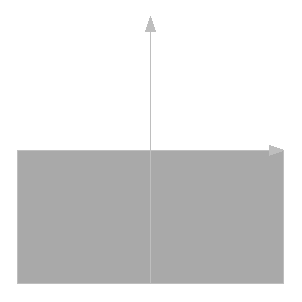
\includegraphics[scale=0.5]{half_plane.eps}
    \end{minipage}
    \begin{minipage}[c]{0.1\textwidth}
        \centering
        \LARGE{$\mapsto$}
    \end{minipage}
    \begin{minipage}[c]{0.45\textwidth}
        \centering
        \includegraphics[scale=0.5]{round.eps}
    \end{minipage}
    \label{fig:23.2}
    \caption{$\Img z > 0 \mapsto \left| z \right| < 1$}
\end{figure}
\nonum
Возьмем любую $z_0: \ \Img z_0 > 0$. Пусть $z_0 \mapsto 0$, а $\ol{z_0} \mapsto
\infty$.
\\
Тогда
\begin{align*}
    & w = A\frac{z-z_0}{z-\ol{z_0}}
\end{align*}
Отыщем теперь $A$. Граница отображается на границу. Возьмем $x \in \RR$, она
должна отображаться на единичную окружность. Тогда
\begin{align*}
    & 1 = \abs{w} = \abs{A\frac{x-z_0}{x-\ol{z_0}}} = \left| A \right| \Rightarrow A = e^{i\alpha}
\end{align*}
Итак,
\begin{equation}\label{(23.6)}
    w = e^{i \alpha}\frac{z-z_0}{z-\ol{z_0}}
\end{equation}
\Example
Отобразить с помощью ДЛО области (см. рис.).
\\
\begin{figure}[h!]
    \begin{minipage}[c]{0.45\textwidth}
        \centering
        \includegraphics[scale=0.5]{round.eps}
    \end{minipage}
    \begin{minipage}[c]{0.1\textwidth}
        \centering
        \LARGE{$\mapsto$}
    \end{minipage}
    \begin{minipage}[c]{0.45\textwidth}
        \centering
        \includegraphics[scale=0.5]{round.eps}
    \end{minipage}
    \label{fig:23.3}
    \caption{$\left| z \right| < 1 \mapsto \left| z \right| < 1$}
\end{figure}
\nonum
Возьмем произвольную $z_0$ и отобразим ее в ноль; тогда симметричная $z_0^* =
\dst \frac{1}{\ol{z_0}}$ перейдет в $\infty$.
\\
Тогда
\begin{align*}
    & w = A\frac{z-z_0}{z-\dst \frac{1}{\ol{z_0}}} = \tilde{A}\frac{z-z_0}{1 - z\ol{z_0}}
\end{align*}
Граница перейдет в границу, а значит,
\begin{align*}
    & 1 = \abs{w} = \abs{\tilde{A}\frac{e^{i \varphi}-z_0}{1 - e^{i \varphi}\ol{z_0}}} = \abs{\tilde{A}\frac{e^{i \varphi}-z_0}{e^{-i \varphi}-\ol{z_0}}} = \abs{\tilde{A}}
\end{align*}
Итак,
\begin{equation}\label{(23.7)}
    w = e^{i \alpha}\frac{z-z_0}{1 - z\ol{z_0}}
\end{equation}
\Example
Отобразить с помощью ДЛО три различные точки $z_1, z_2, z_3$ в три точки $w_1,
w_2,w_3$.
\nonum
Заметим, что условиям удовлетворяет отображение вида
\begin{equation}\label{(23.8)}
    h(z) = \frac{z-z_1}{z-z_2} \cdot \frac{z_3-z_2}{z_3-z_1} = \frac{w-w_1}{w-w_2} \cdot \frac{w_3-w_2}{w_3-w_1} = g(w)
\end{equation}
\begin{align*}
  & w = f(z) = g^{-1}(h(z))
\end{align*}
Существование получено. Докажем единственность.
\\
Пусть для начала $f(z_k) = z_k$, тогда
\begin{align*}
  & \frac{az_k + b}{cz_k+d} = z_k
\end{align*}
\begin{align*}
  & cz^2_k + (d-a)z_k - b = 0
\end{align*}
Значит, поскольку квадратное уравнение имеет три решения, все его коэффициенты
равны нулю. Значит, $f(z) = z$.
\\
Пусть существуют $f_1(z)$, $f_2(z)$, причем $f_1(z_k) = f_2(z_k) = w_k$; тогда
$z_k = f_1^{-1}(f_2(z_k))$, тогда по групповому свойству $f_1^{-1}(z) =
f_2^{-1}(z)$, а значит, $f_1(z) = f_2(z)$.
\Example
Отобразить с помощью ДЛО области (см. рис.).
\\
\begin{figure}[h!]
    \begin{minipage}[c]{0.45\textwidth}
        \centering
        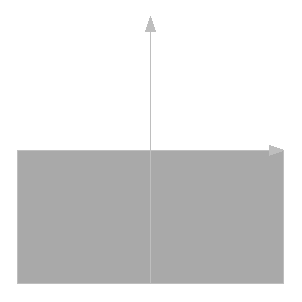
\includegraphics[scale=0.5]{half_plane.eps}
    \end{minipage}
    \begin{minipage}[c]{0.1\textwidth}
        \centering
        \LARGE{$\mapsto$}
    \end{minipage}
    \begin{minipage}[c]{0.45\textwidth}
        \centering
        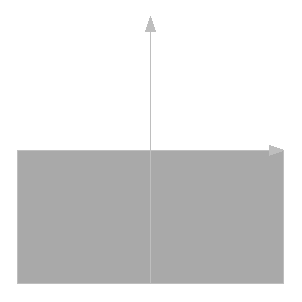
\includegraphics[scale=0.5]{half_plane.eps}
    \end{minipage}
    \label{fig:23.4}
    \caption{$\Img z > 0 \mapsto \Img z > 0$}
\end{figure}
\nonum
Пусть $x_1, x_2, x_3 \in \RR$, $x_1 < x_2 < x_3$, $u_1, u_2, u_3 \in \RR$, $u_1
< u_2 < u_3$, построим отображение $f(x_k) = u_k$. по примеру $3$ такое
отображение существует и единственно, границу оно переводит в границу. Из
свойства сохранения углов следует сохранение ориентации границы. Рассматривая
\eqref{(23.8)}, получаем все действительные  коэффициенты, т.~е. $a, b, c, d \in
\RR$, тогда $\forall x \in \RR \ \argm w'(x) = 0 \Rightarrow w'(x) > 0$, т.~е.
\begin{align*}
  & w'(x) = \frac{ad-cb}{(cx+d)^2} > 0 \Leftrightarrow ad-cb > 0
\end{align*}
Итак, необходимо и достаточно, чтобы все коэффициенты ДЛО были действительны,
причем $ad-cb > 0$.
\section{$\S 24.$ Конформные отображения элементарными функциями. Теорема Римама.}
Рассмотрим функции, обладающие локальной однолистностью.
\begin{center}
    \textbf{Степенная функция}
\end{center}
Фиксируем $t > 0$, рассмотрим область $G = \CC \setminus [0;+\infty)$. Пусть
\begin{align*}
  & w = \left| z \right|^t \exp(it \argt z), \ \argt z \in (0, 2 \pi)
\end{align*}
Функция регулярна при любом $t$. Действительно,
\begin{align*}
  & h(z) = \ln \left| z \right| + i \argt_0 z
\end{align*}
регулярна на этой области, а
\begin{align*}
  & w = \exp(t h(z))
\end{align*}
регулярна в этой области, как суперпозиция регулярных функций.
\\
Исследуем теперь однолистность. Рассмотрим
\begin{align*}
  & G_{0,\varphi_0} = \left\{ z \mid \left| z \right| > 0, \ \argt z \in (0; \varphi_0)\right\}
\end{align*}
\begin{align*}
  & l_{\varphi} = \left\{ z \mid z = r e^{i \varphi}, \ r > 0, \ \varphi \in (0, \varphi_0)\right\}
\end{align*}
Тогда
\begin{align*}
  & w(l_\varphi) = \left\{ w \mid w = \rho e^{i t \varphi}, \ \rho > 0 \right\}
\end{align*}
Тогда условие однолистности:
\begin{align*}
  & \begin{cases}
      0 < \varphi_0 < 2 \pi \\
      0 < t \varphi_0 < 2 \pi
  \end{cases}
\end{align*}
Значит, функция конформна на этой области.
\Example
$t = 2$, $w = z^2$.
\\
Условие однолистности: $\varphi_0 \in (0; \pi)$.
\begin{figure}[h!]
    \begin{minipage}[c]{0.45\textwidth}
        \centering
        \includegraphics[scale=0.5]{half_round.eps}
    \end{minipage}
    \begin{minipage}[c]{0.1\textwidth}
        \centering
        \LARGE{$\mapsto$}
    \end{minipage}
    \begin{minipage}[c]{0.45\textwidth}
        \centering
        \includegraphics[scale=0.5]{cut_rnd.eps}
    \end{minipage}
    \label{fig:24.1}
\end{figure}
\\
Заметим, что данный полукруг содержится в $G_{0, \pi}$~--- области
однолистности, значит, функция будет однолистна.
\Example
$t = 2$, $w = z^2$.
\\
Условие однолистности: $\varphi_0 \in (0; \pi)$.
\begin{figure}[h!]
    \begin{minipage}[c]{0.45\textwidth}
        \centering
        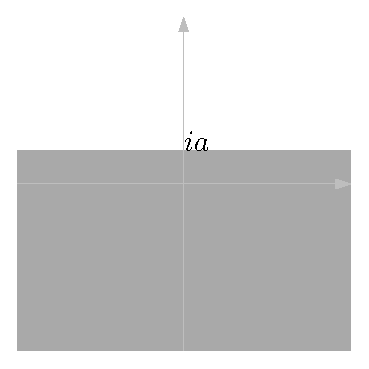
\includegraphics[scale=0.5]{top.eps}
    \end{minipage}
    \begin{minipage}[c]{0.1\textwidth}
        \centering
        \LARGE{$\mapsto$}
    \end{minipage}
    \begin{minipage}[c]{0.45\textwidth}
        \centering
        
\includegraphics[scale=0.5]{parabola.eps}
    \end{minipage}
    \label{fig:24.2}
\end{figure}
\\
Заметим, что данная полуплоскость содержится в $G_{0, \pi}$~--- области
однолистности, значит, функция будет однолистна. Зная, что граница переходит в
границу, отыщем $w(x+ia)$.
\begin{align*}
  & w(x+ia) = (x+ia)^2 = x^2 - a^2 + 2ixa
\end{align*}
\begin{align*}
  & \begin{cases}
      u = x^2 - a^2 \\
      v = 2xa
  \end{cases} \Rightarrow u  = \left( \frac{v}{2a} \right)^2 - a^2
\end{align*}
Поскольку $0$ не лежит в полуплоскости, искомая область будет внешностью
параболы.
\Example
$w = \left| z \right|^{\frac{1}{2}}\exp \left(\dst \frac{i}{2}\argt z\right)$.
\begin{figure}[h!]
    \begin{minipage}[c]{0.45\textwidth}
        \centering
        
\includegraphics[scale=0.5]{parabola.eps}
    \end{minipage}
    \begin{minipage}[c]{0.1\textwidth}
        \centering
        \LARGE{$\mapsto$}
    \end{minipage}
    \begin{minipage}[c]{0.45\textwidth}
        \centering
        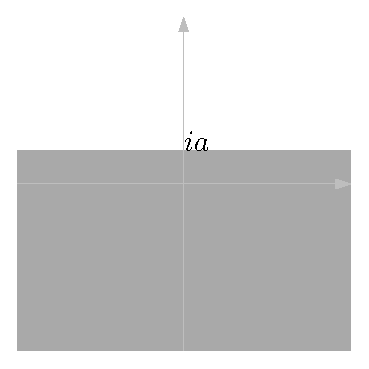
\includegraphics[scale=0.5]{top.eps}
    \end{minipage}
    \label{fig:24.3}
\end{figure}
Обратное к примеру $2$ отображение.
\begin{center}
    \textbf{Экспонента}
\end{center}
Всюду регулярна, но для однолистности необходимо, чтобы не было отличающихся на
$2 i \pi$ элементов (в силу периодичности).
\begin{figure}[h!]
    \centering
    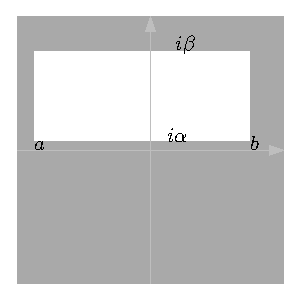
\includegraphics[scale=0.75]{odn_exp.eps}
    \label{fig:24.4}
    \caption{Область однолистности экспоненты}
\end{figure}
\begin{align*}
  & \begin{cases}
      -\infty \leq a \leq b \leq \infty \\
      0 \leq \beta - \alpha < 2 \pi
  \end{cases}
\end{align*}
\Example
\begin{figure}[h!]
    \begin{minipage}[c]{0.45\textwidth}
        \centering
        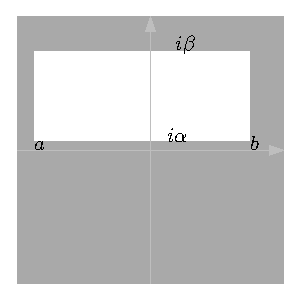
\includegraphics[scale=0.75]{odn_exp.eps}
    \end{minipage}
    \begin{minipage}[c]{0.1\textwidth}
        \centering
        \LARGE{$\mapsto$}
    \end{minipage}
    \begin{minipage}[c]{0.45\textwidth}
        \centering
        
\includegraphics[scale=0.5]{obraz_exp.eps}
    \end{minipage}
    \label{fig:24.5}
\end{figure}
Пусть $z = x+iy_0$, фиксированный $y_0 \in (\alpha,\beta)$. Тогда $\forall x \in
(a,b)$
\begin{align*}
  & f(z) = te^{iy_0}, \ t \in \left( e^{a}, e^{b} \right)
\end{align*}
\Example
~
\\
\begin{figure}[h!]
    \begin{minipage}[c]{0.45\textwidth}
        \centering
        \includegraphics[scale=0.5]{polupolosa.eps}
    \end{minipage}
    \begin{minipage}[c]{0.1\textwidth}
        \centering
        \LARGE{$\mapsto$}
    \end{minipage}
    \begin{minipage}[c]{0.45\textwidth}
        \centering
        \includegraphics[scale=0.5]{half_round.eps}
    \end{minipage}
    \label{fig:24.6}
    \caption{Перевод полуполосы в полуокружность.}
\end{figure}
Вертикальная черта переходит в полуокружность, верхняя граница~--- в отрезок
$[-1;0]$, нижняя граница~--- в отрезок $[0;1]$.
\Example
~
\\
\begin{figure}[h!]
    \begin{minipage}[c]{0.45\textwidth}
        \centering
        \includegraphics[scale=0.5]{d_polupol.eps}
    \end{minipage}
    \begin{minipage}[c]{0.1\textwidth}
        \centering
        \LARGE{$\mapsto$}
    \end{minipage}
    \begin{minipage}[c]{0.45\textwidth}
        \centering
        \includegraphics[scale=0.5]{out_rnd.eps}
    \end{minipage}
    \label{fig:24.7}
    \caption{Перевод полуполосы во внешность полуокружности.}
\end{figure}

    \begin{flushright}
    \textit{Лекция 19 (от 09.11)}
\end{flushright}
\begin{center}
    \textbf{Функция Жуковского}
\end{center}
\begin{equation}\label{(24.1)}
    w = \frac{1}{2}\left( z+\frac{1}{z} \right)
\end{equation}
Заметим, что $0$ и $\infty$~--- полюсы $1$ порядка, $\pm 1$~--- нули
производной.
\\
В каждой точке $z \not \in \left\{0, \pm 1,\infty \right\}$ функция конформна. В
точке $0$
\begin{align*}
  & g(z) = \frac{1}{w(z)} = \frac{2z}{z^2+1}
\end{align*}
Эта функция в нуле регулярна и имеет ненулевую производную, а значит, конформна
в нуле. В точке $\infty$
\begin{align*}
  & \varphi(z) = w\left( \frac{1}{z} \right) = \frac{1}{2}\left( \frac{1}{z} + z \right)
\end{align*}
Заметим, что это та же $w$, и в силу конформности в нуле конформна и на
бесконечности. В остальных точках проверим однолистность.
\begin{align*}
  & \frac{1}{2}\left( z_1 + \frac{1}{z_1} \right) - \frac{1}{2}\left( z_1 + \frac{1}{z_1} \right) = 0
\end{align*}
\begin{align*}
  & (z_1-z_2) \left( 1-\frac{1}{z_1z_2} \right)
\end{align*}
\begin{align*}
  & \left[ \begin{matrix}
          z_1=z_2 \\
          z_1z_2 = 1
      \end{matrix} \right.
\end{align*}
Область однолистности $G$: $\pm 1 \not \in G$, $\forall z \in G \ \dst
\frac{1}{z} \not \in G$.
\Example
Функция $w = \dst \frac{1}{z}$ задает две симметрии: относительно единичной
окружности и относительно действительной оси. Соответственно, области
однолистности:
\begin{itemize}
    \item $\left| z \right| < 1$
    \item $\left| z \right| > 1$
    \item $\Img z > 0$
    \item $\Img z < 0$
\end{itemize}
Пусть $z = e^{i \varphi}$, тогда функция Жуковского:
\begin{align*}
  & w = \frac{1}{2}\left( e^{i \varphi} + e^{-i\varphi}\right)
\end{align*}
\begin{equation}\label{(24.2)}
    \begin{cases}
        u = \frac{1}{2}\left( r+\frac{1}{r} \right)\cos \varphi \\
        v = \frac{1}{2}\left( r-\frac{1}{r} \right)\sin \varphi
    \end{cases}
\end{equation}
\Example
~
\begin{itemize}
    \item Пусть задана окружность
    \begin{align*}
      \gamma_r = \left\{ z: \left| z \right| = r, \ r \neq 1\right\}
    \end{align*}
    \begin{align*}
      & \frac{u^2}{a^2} + \frac{v^2}{b^2} = 1, \ a = \frac{1}{2}\left( r + \frac{1}{r} \right), \ b = \frac{1}{2}\left|  r - \frac{1}{r} \right|
    \end{align*}
    \begin{align*}
      & a^2+b^2 = c^2 = 1
    \end{align*}
    Такая окружность переходит в эллипс с фокусами в $\pm 1$, действительной
    полуосью $a$ и мнимой $b$.
    \item Пусть задан луч
    \begin{align*}
      l_\varphi = \left\{ z \mid z = re^{i\varphi}, \ r > 0\right\}, \ \varphi \in [-\pi;\pi) \setminus \left\{ 0, \pm \frac{\pi}{2}, -\pi \right\}
    \end{align*}
    \begin{equation}\label{(24.3)}
        \frac{u^2}{\cos^2 \varphi} - \frac{v^2}{\sin^2\varphi} = 1
    \end{equation}
    Такой луч переходит в гиперболу с фокусами в $\pm 1$.
    \begin{itemize}
        \item $\varphi \in \left( 0; \dst \frac{\pi}{2} \right)$~--- отображение
        в правую ветвь гиперболы, движение по ней вверх.
        \item $\varphi \in \left(\dst \frac{\pi}{2}; \pi \right)$~---
        отображение в левую ветвь гиперболы, движение по ней вверх.
        \item $\varphi \in \left( - \dst \frac{\pi}{2}; 0 \right)$~---
        отображение в правую ветвь гиперболы, движение по ней вниз.
        \item $\varphi \in \left( -\pi; -\dst \frac{\pi}{2} \right)$~---
        отображение в левую ветвь гиперболы, движение по ней вниз.
    \end{itemize}
\end{itemize}
\Example
~
\\
\begin{figure}[h!]
    \begin{minipage}[c]{0.45\textwidth}
        \centering
        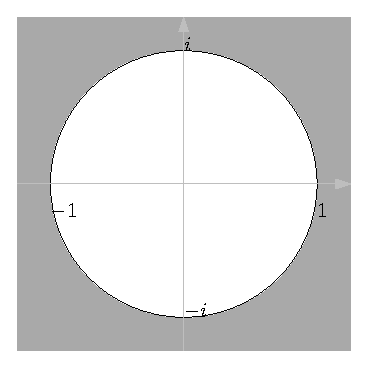
\includegraphics[scale=0.75]{rnd_in.eps}
    \end{minipage}
    \begin{minipage}[c]{0.1\textwidth}
        \centering
        \LARGE{$\mapsto$}
    \end{minipage}
    \begin{minipage}[c]{0.45\textwidth}
        \centering
        \includegraphics[scale=0.5]{pm1.eps}
    \end{minipage}
    \label{fig:24.10}
    \caption{Перевод единичного круга в $\CC \setminus [-1;1]$}
\end{figure}
\FloatBarrier
\Example
~
\\
\begin{figure}[h!]
    \begin{minipage}[c]{0.45\textwidth}
        \centering
        \includegraphics[scale=0.75]{rnd_out.eps}
    \end{minipage}
    \begin{minipage}[c]{0.1\textwidth}
        \centering
        \LARGE{$\mapsto$}
    \end{minipage}
    \begin{minipage}[c]{0.45\textwidth}
        \centering
        \includegraphics[scale=0.5]{pm1.eps}
    \end{minipage}
    \label{fig:24.11}
    \caption{Перевод внешности единичного круга в $\CC \setminus [-1;1]$}
\end{figure}
\FloatBarrier
\Example
~
\\
\begin{figure}[h!]
    \begin{minipage}[c]{0.45\textwidth}
        \centering
        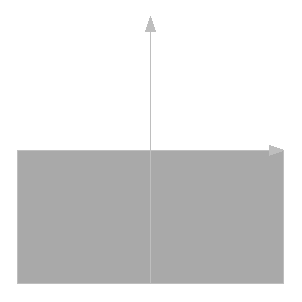
\includegraphics[scale=0.75]{half_plane.eps}
    \end{minipage}
    \begin{minipage}[c]{0.1\textwidth}
        \centering
        \LARGE{$\mapsto$}
    \end{minipage}
    \begin{minipage}[c]{0.45\textwidth}
        \centering
        \includegraphics[scale=0.5]{pm1out.eps}
    \end{minipage}
    \label{fig:24.12}
    \caption{Перевод верхней полуплоскости в $\CC \setminus ((-\infty;-1]\cup[1;+\infty)$}
\end{figure}
\FloatBarrier
\Example
~
\\
\begin{figure}[h!]
    \begin{minipage}[c]{0.45\textwidth}
        \centering
        \includegraphics[scale=0.75]{half_plane_t.eps}
    \end{minipage}
    \begin{minipage}[c]{0.1\textwidth}
        \centering
        \LARGE{$\mapsto$}
    \end{minipage}
    \begin{minipage}[c]{0.45\textwidth}
        \centering
        \includegraphics[scale=0.5]{pm1out.eps}
    \end{minipage}
    \label{fig:24.13}
    \caption{Перевод нижней полуплоскости в $\CC \setminus ((-\infty;-1]\cup[1;+\infty)$}
\end{figure}
\FloatBarrier
Отыщем обратную функцию Жуковского.
\begin{align*}
  & w = \frac{1}{2}\left( z+\frac{1}{z} \right) \Rightarrow z^2 - 2wz + 1 = 0
\end{align*}
\begin{align*}
  & z = w \pm g(w), \ g(w) \in \sqrt{w^2-1}
\end{align*}
\Example
Ветвь обратной функции Жуковского, где $g \sim w$ при $w \to \infty$, $z = w -
g(w)$, выполняет следующее преобразование:
\\
\begin{figure}[h!]
    \begin{minipage}[c]{0.45\textwidth}
        \centering
        \includegraphics[scale=0.5]{pm1.eps}
    \end{minipage}
    \label{fig:24.14}
    \begin{minipage}[c]{0.1\textwidth}
        \centering
        \LARGE{$\mapsto$}
    \end{minipage}
        \begin{minipage}[c]{0.45\textwidth}
        \centering
        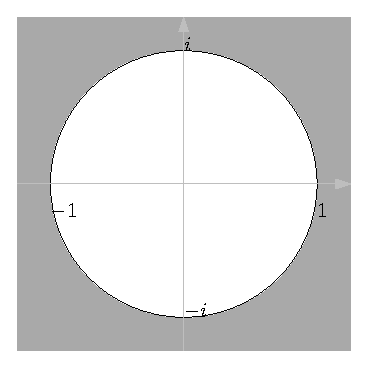
\includegraphics[scale=0.75]{rnd_in.eps}
    \end{minipage}
    \caption{Перевод $\CC \setminus [-1;1]$ в единичный круг}
\end{figure}
\FloatBarrier
\Example
Ветвь обратной функции Жуковского, где $g \sim w$ при $w \to \infty$, $z = w +
g(w)$, выполняет следующее преобразование:
\\
\begin{figure}[h!]
        \begin{minipage}[c]{0.45\textwidth}
        \centering
        \includegraphics[scale=0.5]{pm1.eps}
    \end{minipage}
    \begin{minipage}[c]{0.1\textwidth}
        \centering
        \LARGE{$\mapsto$}
    \end{minipage}
        \begin{minipage}[c]{0.45\textwidth}
        \centering
        \includegraphics[scale=0.75]{rnd_out.eps}
    \end{minipage}
    \label{fig:24.15}
    \caption{Перевод $\CC \setminus [-1;1]$ во  внешность единичного круга}
\end{figure}
\FloatBarrier
\Example
Ветвь обратной функции Жуковского, где $g(0) = i$, $z = w - g(w)$, выполняет
следующее преобразование:
\\
\begin{figure}[h!]
        \begin{minipage}[c]{0.45\textwidth}
        \centering
        \includegraphics[scale=0.5]{pm1out.eps}
    \end{minipage}
    \begin{minipage}[c]{0.1\textwidth}
        \centering
        \LARGE{$\mapsto$}
    \end{minipage}
    \begin{minipage}[c]{0.45\textwidth}
        \centering
        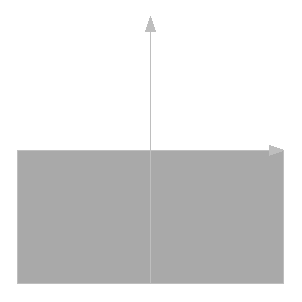
\includegraphics[scale=0.75]{half_plane.eps}
    \end{minipage}
    \label{fig:24.16}
    \caption{Перевод $\CC \setminus (-\infty;-1]\cup[1;+\infty)$ в верхнюю полуплоскость}
\end{figure}
\FloatBarrier
\Example
Ветвь обратной функции Жуковского, где $g(0) = i$, $z = w + g(w)$, выполняет
следующее преобразование:
\\
\begin{figure}[h!]
        \begin{minipage}[c]{0.45\textwidth}
        \centering
        \includegraphics[scale=0.5]{pm1out.eps}
    \end{minipage}
    \begin{minipage}[c]{0.1\textwidth}
        \centering
        \LARGE{$\mapsto$}
    \end{minipage}
    \begin{minipage}[c]{0.45\textwidth}
        \centering
        \includegraphics[scale=0.75]{half_plane_t.eps}
    \end{minipage}
    \label{fig:24.17}
    \caption{Перевод $\CC \setminus (-\infty;-1]\cup[1;+\infty)$ в нижнюю полуплоскость}
\end{figure}
\FloatBarrier
\begin{center}
    \textbf{Теорема Римана}
\end{center}
$\CC$ нельзя конформно отобразить на единичный круг. Действительно, функция (в
предположении существования) будет ограничена, регулярна (в силу определенности
на всей комплексной плоскости она обязана быть целой), значит, по теореме
Лиувилля это константа, что не является требуемым отображением.
\theorem
Общий вид конформного отображения $B_1(0) \mapsto B_1(0)$:
\begin{equation}\label{(24.4)}
    f(z) = e^{i\beta}\frac{z-a}{1-z\ol{a}}
\end{equation}
\pr
Если $f$ удовлетворяет \eqref{(24.4)}, то $f: B_1(0) \mapsto B_1(0)$ есть ДЛО, а
значит, оно конформно.
\\
Пусть теперь $g: B_1(0) \mapsto B_1(0)$~--- некоторое конформное отображение.
Докажем, что такая функция удовлетворяет \eqref{(24.4)}.
\\
Заметим:
\begin{align*}
  \exists w_0 \in B_1(0): \ g(0) = w_0
\end{align*}
Расмотрим теперь
\begin{align*}
  h(w) = \frac{w-w_0}{1-w\ol{w_0}}, \ h(w_0) = 0, \ h:B_1(0)\mapsto B_1(0)
\end{align*}
Положим
\begin{align*}
  f(z) = h(g(z))
\end{align*}
$f$ регулярна, как суперпозиция регулярных функций, и причем $f(0) = 0$,
$f:B_1(0) \mapsto B_1(0)$. Тогда по лемме Шварца $\forall z \in B_1(0) \ \left|
    f(z) \right|\leq \left| z \right|$.
\\
Тогда $f^{-1}$ таже будет регулярна, $f^{-1}(0) = 0$, $f^{-1}: B_1(0) \mapsto
B_1(0)$. Тогда по лемме Шварца $\forall w \in B_1(0) \ \left| f^{-1}(w)
\right|\leq \left| w \right|$. Подставляя сюда $w = f(z)$, получим $\left| z
\right| \leq \left| f(z) \right|$, т.~е. $\left| z \right| = \left| f(z)
\right|$, и по лемме Шварца выполняется $f(z) = e^{i\alpha}z$.
\\
Тогда $g(z)$~--- ДЛО. Проверим, что $g$ имеет вид \eqref{(24.4)}.
\begin{align*}
& e^{i\alpha}z = h^{-1}(g(z)); \ \exists z_0 \in B_1(0): \ g(z_0) = 0
\end{align*}
\begin{align*}
& e^{i\alpha} = (h^{-1})'(0)(g'(z_0)) = \frac{g'(z_0)}{h'(w_0)}
\end{align*}
\begin{align*}
& \alpha \in \Arg g'(z_0) - \Arg h'(w_0)
\end{align*}
\begin{align*}
& h'(w_0) = \left.\frac{1-w\ol{w_0}+\ol{w_0}(w-w_0)}{(1-w\ol{w_0})^2}\right|_{w=w_0} = 1 - \left| w_0 \right|^2 > 0 \Rightarrow 0 \in \Arg h'(w_0)
\end{align*}
\begin{align*}
& \alpha \in \Arg g'(z_0)
\end{align*}
Рассмотрим теперь 
\begin{align*}
& g_1(z) = e^{i\alpha}\frac{z-z_0}{1-z\ol{z_0}}
\end{align*}
\begin{align*}
&\varphi(z) = g(g_1^{-1}(w)): B_1(0) \mapsto B_1(0)
\end{align*}
\begin{align*}
&\varphi(g_1(z)) = g(w), \ \varphi(0) = 0, \ \Arg \varphi'(0) + \Arg g_1'(0) = \Arg g'(z_0)
\end{align*}
Дифференцируя,
\begin{align*}
& \alpha \in \Arg g_1(0), \ 0 \in \Arg \varphi'(0)
\end{align*}
По лемме Шварца для прямой и обратной функций
\begin{align*}
& \left| \varphi(z) \right| = \left| z \right| \Rightarrow \varphi(z) = z
\end{align*}
(в силу $0 \in \Arg \varphi'(0)$). Но тогда $g_1(z) = g(z)$, и теорема
доказана.
\lemma 
Пусть область $G\subseteq \CC$ такова, что существует конформное $f_0: G \mapsto
B_1(0)$. Тогда любое конформное отображение $G$ на $B_1(0)$ имеет вид
\begin{align*}
  & f(z) = h(f_0(z))
\end{align*}
причем $h$ имеет вид \eqref{(24.4)}.
\pr
Пусть $f_1: G \mapsto B_1(0)$~--- конформное. Рассмотрим 
\begin{align*}
  & \varphi(w) = f_1(f_0^{-1}(w)): B_1(0) \mapsto B_1(0)
\end{align*}
Оно конформно как суперпозиция конформных. По теореме $1$ это ДЛО,
уловлетворяющее \eqref{(24.4)}. Поскольку
\begin{align*}
& f_1(z) = \varphi(f_0(z))
\end{align*}
то лемма доказана.
\theorem (единственности конформных отображений)
Пусть $G$ такова, что существует конформное $f_0:G \mapsto B_1(0)$. Тогда
множество всех конформных отображений $G \mapsto B_1(0)$ зависит от трех
действительных параметров. В частности, такое отображение единственно, если
выполнены условия:
\begin{equation}\label{(24.5)}
f(z_0) = 0, \ \argt f'(z_0) = \alpha \in [0;2\pi), \ z_0 \in G
\end{equation}
\pr
Из леммы $1$ и теоремы $1$ следует утверждение о трех параметрах.
\\
Докажем теперь единственность. Допустим, от противного, существуют $f_1$, $f_2$,
удовлетворяющие \eqref{(24.5)}. Пусть
\begin{align*}
  & \varphi(w) = f_1(f_2^{-1}(w)), \ \varphi(f_2(z)) = f_1(z), \ \varphi(0) = 0
\end{align*}
Значит, $\varphi(z)$ будет ДЛО по лемме $1$. Дифференцируя в $z_0$, имеем
\begin{align*}
    & \argt \varphi'(0) + \Arg f_2'(z_0) = \Arg f_1'(z_0)
\end{align*}
\begin{align*}
  & 0 \in \Arg \varphi'(0) \Rightarrow \varphi(0) = 0, \ z_0 = 0, \ \alpha = 0
\end{align*}
\begin{align*}
  & \varphi(z) = z \Rightarrow f_1(z) = f_2(z)
\end{align*}
\theorem (Римана)
Пусть $G$~--- область в $\CCC$, граница которой содержит более одной точки.
Тогда существует конформное $f: G \mapsto B_1(0)$.
\corollary
Если $G_1 \subseteq \CCC$, $G_2 \subseteq \CCC$, и ганицы каждой содержат более
одной точки, то существует конформное обображение $G_1$ на $G_2$.
\pr
Пусть $f_1: G_1 \mapsto B_1(0)$, $f_2: G_2 \mapsto B_1(0)$, тогда искомое
отображение $\varphi(z) = f_1(f_2^{-1}(z)): G_1 \mapsto G_2$.
\theorem (принцип соответствия границ)
Пусть $G_1, G_2$~--- ограниченные односвязные области в $\CC$ с кусочно гладкими
границами $\Gamma_1, \Gamma_2$. Пусть $f: G_1 \mapsto G_2$~--- конформное; тогда
существует непрерывное продолжение $\tilde{f}$ такое, что оно отображает
$\Gamma_1$ на $\Gamma_2$ с сохранением ориентации.
    \begin{flushright}
    \textit{Лекция 20 (от 10.11)}
\end{flushright}
\section{$\S 25.$ Принцип симметрии.}
\theorem
Пусть заданы области $G$, $G^*$ в верхней полуплоскости с кусочно гладкими
границами $\Gamma$, $\Gamma^*$. Пусть границы содержат конечное чило интервалов
действительной оси $l_1, \dots, l_n$, $l_1^*, \dots, l_n^*$. Пусть $\tilde{G}$,
$\tilde{G^*}$~--- симметричные относительно действительной оси области. Пусть
$f: G \cup \dst \bigcup_{s=1}^n l_s \mapsto G^*\cup \dst \bigcup_{s=1}^n l_s^*$
конформна на $G$ и непрерывна на $G \cup \dst \bigcup_{s=1}^n l_s$ взамно
однозначно отображает $\forall s \in \left\{ 1, \dots, n \right\} \ l_s \mapsto
l_s^*$. Тогда существует (аналитическое) продолжение $f$ на область $G \cup \dst
\bigcup_{s=1}^n l_s \cup \tilde{G}$, конформно отображающее ее на $G^* \cup \dst
\bigcup_{s=1}^n l_s^* \cup \tilde{G^*}$.
\begin{figure}[h!]
    \begin{minipage}[c]{0.5\textwidth}
        \centering
        
\includegraphics[scale=0.75]{1st.eps}
    \end{minipage}
    \begin{minipage}[c]{0.5\textwidth}
        \centering
        
\includegraphics[scale=0.75]{2nd.eps}
    \end{minipage}
    \label{fig:25.1}
\end{figure}
\pr
Зададим функцию $F$ (искомое продолжение).
\begin{equation}\label{(25.1)}
    F(z) = \begin{cases}
        f(z), \ z \in G \cup \bigcup_{s=1}^n l_s \\
        \ol{f(\ol{z})}, \ z \in \tilde{G}
    \end{cases}
\end{equation}
Докажем дифференцируемость. Пусть $z_0 \in \tilde{G}$; тогда
\begin{align*}
  & \exists \varepsilon > 0: \ \forall \Delta z: \ \left| \Delta z \right| < \varepsilon \ z_0+\Delta z \in G
\end{align*}
\begin{align*}
  & \frac{F(z_0+\Delta z) - F(z_0)}{\Delta z} = \frac{\ol{f}(\ol{z_0+\Delta z}) - \ol{f}(\ol{z_0})}{\Delta z} = \ol{\frac{f(\ol{z_0}+\ol{\Delta z}) - f(\ol{z_0})}{\ol{\Delta z}}}
\end{align*}
Тогда
\begin{align*}
  & \ol{z_0} \in G, \ \ol{z_0} +\ol{\Delta z} \in G, \ \exists f'(\ol{z_0}) = \lim_{\Delta z \to 0} \frac{f(\ol{z_0}+\ol{\Delta z}) - f(\ol{z_0})}{\ol{\Delta z}}
\end{align*}
\begin{align*}
  & \exists F'(z_0) = \ol{f'(\ol{z_0})}
\end{align*}
Пусть теперь $x_0 \in l_s$. Докажем, что $F(z)$ непрерывна в $x_0$. Рассмотрим
нижний полукруг окрестности.
\begin{align*}
  & \lim_{z \os{\tilde{G}}{\to} x_0}F(z) = \lim_{\ol{z} \os{G}{\to} x_0}\ol{f(\ol{z})} = \ol{\lim_{\ol{z} \os{G}{\to} x_0}f(\ol{z})} = \ol{f(x_0)} = f(x_0) \in l_s^*
\end{align*}
Аналогично находится предел по верхнему полукругу.
\\
Тогда по теореме о стирании разреза $F(z)$ регулярна в $x_0$ и, значит,
регулярна во всей объединенной области.
\\
Докажем, наконец, однолистность. Область $G$ отображалась однолистно, как и
интервалы; каждая точка $\tilde{G}$ соответствует единственной точке $G$, как и
$\tilde{G^*}$ и $G^*$, а значит, отображение однолистно и на оставшейся части.
\corollary
принцип симметрии можнообобщить на симметрии относительно любой прямой или
окружности.
\pr
Всякую такую кривую можем перевести в действительную ось (область~--- в верхнюю
полуплоскость), применить принцип симметрии и перевести обратно.
\Example
Найти преобразование, переводящее данные области.
\begin{figure}[h!]
    \begin{minipage}[c]{0.45\textwidth}
        \centering
        \includegraphics[scale=0.75]{ex24_1.eps}
    \end{minipage}
    \begin{minipage}[c]{0.1\textwidth}
        \centering
        \LARGE{$\mapsto$}
    \end{minipage}
    \begin{minipage}[c]{0.45\textwidth}
        \centering
        \includegraphics[scale=0.5]{half_plane.eps}
    \end{minipage}
    \label{fig:25.1}
\end{figure}
Воспользовавшись принципом симметрии, рассмотрим лишь правую часть вместе с
мнимой осью. Используя $w_1 = z^4$, получим $\CC \setminus[-4;+\infty)$, причем
функция будет непрерывно продлена на нижний край разреза от нуля и до
бесконечности. Применяя $w_2 = w_1+4$, получим $\CC \setminus[0;+\infty)$, причем
функция будет непрерывно продлена на нижний край разреза от $4$ и до
бесконечности. При помощи $w_3 = \sqrt{\left| w_2 \right|}\exp \left(
\dst \frac{i}{2}\argt w_2\right)$ получаем верхнюю полуплоскость, а $(-\infty;
-2]$ имеет непрерывное продолжение функции на себе. Затем сдвигаем этот разрез:
$w_4 = w_3+2$, и извлекаем корень: $w_5 = \sqrt{\left| w_4 \right|}\exp \left(
    \dst \frac{i}{2}\argt w_4\right)$. По принципу симметрии можем раскрыть все
до полуплоскости.
\begin{center}
    \begin{tabular}{cccc}
      \includegraphics[scale=0.75]{ex24_1.eps} & $\Rightarrow$ & \includegraphics[scale=0.75]{2511.eps} & $\mapsto$ \\
    \end{tabular}
\end{center}
\begin{center}
    \begin{tabular}{cccc}
      \includegraphics[scale=0.75]{2512.eps} & $\mapsto$ & \includegraphics[scale=0.75]{2513.eps} & $\mapsto$ \\
    \end{tabular}
\end{center}
\begin{center}
    \begin{tabular}{cccc}
      \includegraphics[scale=0.75]{2514.eps} & $\mapsto$ & \includegraphics[scale=0.75]{2515.eps} & $\mapsto$ \\
    \end{tabular}
\end{center}
\begin{center}
    \begin{tabular}{cccc}
      \includegraphics[scale=0.75]{2516.eps} & $\Rightarrow$ & \includegraphics[scale=1]{half_plane.eps} & \\
    \end{tabular}
\end{center}
\Example
Найти преобразование, переводящее данные области.
\begin{align*}
  & G = \left\{ z = x+iy \mid y^2 < 2p \left( x+\frac{p}{2} \right) \right\}, \ p > 0
\end{align*}
\begin{figure}[h!]
    \begin{minipage}[c]{0.45\textwidth}
        \centering
        \includegraphics[scale=0.75]{2520.eps}
    \end{minipage}
    \begin{minipage}[c]{0.1\textwidth}
        \centering
        \LARGE{$\mapsto$}
    \end{minipage}
    \begin{minipage}[c]{0.45\textwidth}
        \centering
        \includegraphics[scale=0.5]{half_plane.eps}
    \end{minipage}
    \label{fig:25.1}
\end{figure}
Воспользовавшись принципом симметрии, рассмотрим лишь верхнюю часть вместе с
действительной осью. Используя $w_1 = \sqrt{\left| z \right|}\exp \left(\dst
    \frac{i}{2}\argt z\right)$, получаем полуполосу. Растянем эту полуполосу при
помощи $w_2 = \pi\sqrt{\frac{2}{\pi}}$, экспонентой $w_3 = e^{w_2}$ превратим в
верхнюю полуплоскость с вырезанным единичным полукругом. Функцией Жуковского
$w_4 = dst \frac{1}{2}\left( w_3+\dst\frac{1}{w_4} \right)$ переводим в верхнюю
полуплоскость, но она имеет особый участок $[-1;+\infty)$. По принципу симметрии
можем раскрыть это до плоскости с разрезом по $(-\infty;-1]$, и легко, сдвигая
$w_5 = -w_4+1$ и извлекая корень $w_6 = \sqrt{\left| w_5 \right|}\exp \left(\dst
    \frac{i}{2}\argt w_5\right)$, получаем искомое.
\begin{center}
    \begin{tabular}{cccc}
      \includegraphics[scale=0.75]{2520.eps} & $\Rightarrow$ & \includegraphics[scale=0.75]{2521.eps} & $\mapsto$ \\
    \end{tabular}
\end{center}
\begin{center}
    \begin{tabular}{cccc}
      \includegraphics[scale=0.75]{2522.eps} & $\mapsto$ & \includegraphics[scale=0.75]{2523.eps} & $\mapsto$ \\
    \end{tabular}
\end{center}
\begin{center}
    \begin{tabular}{cccc}
      \includegraphics[scale=0.75]{2524.eps} & $\mapsto$ & \includegraphics[scale=0.75]{2525.eps} & $\Rightarrow$ \\
    \end{tabular}
\end{center}
\begin{center}
    \begin{tabular}{cccc}
      \includegraphics[scale=0.75]{2526.eps} & $\mapsto$ & \includegraphics[scale=1]{2527.eps} & $\mapsto$ \\
    \end{tabular}
\end{center}
\begin{center}
    \begin{tabular}{cccc}
      \includegraphics[scale=0.5]{half_plane.eps} & & & \\
    \end{tabular}
\end{center}
\section{$\S 26.$ Задача Дирихле на плоскости.}
\theorem
Пусть $f: G \mapsto D$ регулярная и непрстоянная. Пусть $\tilde{u}: D \mapsto
\RR$ гармоническая. Тогда $u(z) = \tilde{u}(f(z))$ также гармоническая.
\pr
Пусть $z_0 \in G$~--- произвольная точка. Пусть $f(z_0) = w_0$, и $f(G) =
G^*$~--- также, как известно, область. Тогда
\begin{align*}
  & \exists \varepsilon > 0: B_\varepsilon(w_0) \subseteq G^* \subseteq D
\end{align*}
По теореме $2$ $\S 4$
\begin{align*}
  & \exists h(w): \ \Real h(w) = \tilde{u}(w), \ w \in B_\varepsilon(w_0)
\end{align*}
причем $h$~--- регулярная. Рассмотрим теперь $h(f(z))$ в окрестности
$B_\delta(w_0)$, такой, чо $f\left( B_\delta(z_0) \right) \subseteq
B_\varepsilon(w_0)$. Тогда в этой окрестности $h$ будет регулярной,
$\tilde{u}(w) = \Real h(w)$~--- гармонической, тогда и $u(z) = \tilde{u}(f(z))$
тоже будет гармонической в этой окрестности, а в силу произвольности выбора
$z_0$~--- и на всей области.
\Def
\textbf{Классическим решением задачи Дирихле в области $G$} называется
следующее:
\begin{itemize}
    \item $G$~--- ограниченная односвязная область в $\CC$ с кучочно гладкой
    границей $\Gamma$;
    \item дана непрерывная функция $u_0(z)$ на этой границе;
    \item нужно найти гармоническую функцию $u(z)$ в области $G$, непрерывную на
    ее замыкании и удовлетворяющую условию: $u\Big|_\Gamma = u_0$.
\end{itemize}
\Def
\textbf{Общей задачей Дирихле} называется следующее:
\begin{itemize}
    \item $G$~--- односвязная область в $\CCC$ с кучочно гладкой границей $\Gamma$;
    \item дана непрерывная функция всюду за исключением коненого числа точек
    разрыва $1$ рода $\zeta_1, \dots, \zeta_n$ $u_0(z)$ на этой границе и
    ограниченная на ней за вычетом этих точек;
    \item нужно найти гармоническую функцию $u(z)$ в области $G$, ограниченную
    на ее замыкании, непрерывную на ее замыкании за вычетом этих точек и
    удовлетворяющую условию: $u = u_0$ на границе за вычетом этих точек.
\end{itemize}
\lemma
Лемма доказывается для случая ограниченной области.
\\
Пусть $G$~--- ограниченная односвязная область в $\CC$. Если решение общей
задачи Дирихле существует в этой области с $u_0(z)$ и $\tilde{\Gamma} = \Gamma
\setminus \dst \bigcup_{k=1}^n \left\{ \zeta_k \right\}$, то все значения $u(z)$
лежат на отрезке $\left[ m, M \right]$, где $m = \us{z \in\tilde{\Gamma}}{\inf} u_0(z)$, $M = \us{z \in\tilde{\Gamma}}{\sup}u_0(z)$.
\pr
Пусть $d = \sup \left| z_1-z_2 \right|$, $z_1, z_2 \in G$~--- диаметр множества.
Пусть
\begin{equation}\label{(26.1)}
    U_\varepsilon = M + \varepsilon \sum_{k=1}^n \ln \frac{d}{\left| z-\zeta_k\right|}, \ \varepsilon > 0
\end{equation}
Это гармоническая функция, причем она не меньше $M$ и непрерывна на замыкании
за вычетом точек разрыва, причем
\begin{equation}\label{(26.2)}
    \lim_{z \to \zeta_k} U_\varepsilon(z) = \infty
\end{equation}
Полагая
\begin{align*}
  & \gamma_r^k = \left\{ z \in G: \left| z - \zeta_k \right| = r\right\}
\end{align*}
\begin{equation}\label{(26.3)}
    \lim_{r \to 0}\min \left\{ U_\varepsilon(z) \mid z \in \gamma_r^k \right\} = +\infty
\end{equation}
\begin{align*}
    & \forall z \in \tilde{\Gamma} \ U_\varepsilon(z) > M\geq u_0(z) = u(z)
\end{align*}
Из ограниенности и выполнимости \eqref{(26.3)} для $u(z)$ имеем, чтопри
достаточно малых $r$ на границе области $G_r = G \setminus \dst \bigcup_{k=1}^n
B_r(\zeta_k)$ $U_\varepsilon(z) > U(z)$. По принципу максмума гармонической
функции это соотношение верно и для всей $G_r$.
\\
Фиксируем произвольную  $z \in G$. тогда $\exists r_0: z \in G_{r_0}$, значит,
$U_\varepsilon(z) > u(z)$ на всей $G$. При устремлении $\varepsilon$ к нулю
получаем, что $u(z) \leq M$.
\\
Аналогично можем ограничить сверху гармоническую $-u(z)$ числом $-m$ и получить
искомое.
\Note
Без условия ограниченности области лемма также справедлива.
\corollary
Для случая непостоянной $u_0(z)$ выполняются строгие неравенства.
\pr
От противного: предположим существование внутренней точки области, где $M$
достигается; тогда должна существовать $z_1 \in G: \ u(z_1) > M$ (аналогичнно
доказательству принципа максимума). Противоречие с неравенством, даже нестрогим.    

    \begin{flushright}
    \textit{Лекция 21 (от 16.11)}
\end{flushright}
\theorem
В общей задаче Дирихле при существовании решения в ограниченной области онобудет
единственным. Решение ищем как ограниченную функцию.
\pr
От противного. Допустим, существуют два различных решения $u_1$, $u_2$. Тогда $w
= u_1-u_2 : G \mapsto \RR$, $\Delta w = 0$, $w\Big|_\Gamma = 0$. Тогда по лемме
$1$ $w \equiv 0$.
\Note
Условие ограниченности области является лишь техническим. Условие же
ограниченности функции на области существенно.
\Example
\begin{align*}
  & u(x,y) = \frac{x^2+y^2-2x}{x^2+y^2}
\end{align*}
\begin{align*}
  & G = \left\{ (x,y) \mid x^2+y^2<2x \right\} = \left\{ z: \left| z \right| <1\right\}
\end{align*}
При граничном условии~--- нуле эта функция является решением задачи Дирихле, но
и тождественный нуль также решение. При условии ограниченности эта функция не
подходит.
\begin{center}
    \textbf{Класическая задача Дирихле в круге $B_R(0), \ R > 0$}
\end{center}
\begin{equation}\label{(26.4)}
    \begin{cases}
        \Delta u = 0, \ \left| z \right|< R \\
        u \big|_{\left| z \right| = R} = u_0(z)
    \end{cases}
\end{equation}
причем $u_0(z)$ непрерывна на $\gamma_r$ и решение \eqref{(26.4)} непрерывно на
некотором $B_{R_1}(0), \ R_1 > R$.
\\
Тогда существует регулярная $f: B_{R_1}(0) \mapsto \CC$, что $\Real f(z) =
u(z)$. Тогда по интегральной формуле Коши
\begin{align*}
  & \forall z \in B_R(0) \ f(z) = \frac{1}{2 i \pi} \int_{\gamma_R} \frac{f(\zeta)}{\zeta - z}d\zeta = \frac{1}{2 \pi} \int_{0}^{2\pi} \frac{f(Re^{i\psi})\zeta(\psi)}{\zeta(\psi) - z}d\psi
\end{align*}
Введем теперь симметричную точку $z^* = \dst \frac{R^2}{z}$. Тогда
\begin{align*}
  & \frac{1}{2 i \pi} \int_{\gamma_R} \frac{f(\zeta)}{\zeta - z^*}d\zeta = \frac{1}{2 \pi} \int_{0}^{2\pi} \frac{f(Re^{i\psi})\zeta(\psi)}{\zeta(\psi) - z^*}d\psi = 0
\end{align*}
\begin{align*}
  & f(z) = \frac{1}{2\pi}\int_{0}^{2\pi}f(\zeta(\psi))\left( \frac{\zeta(\psi)}{\zeta(\psi) - z} - \frac{\zeta(\psi)}{\zeta(\psi) - z^*}\right)d\psi = \frac{1}{2\pi}\int_{0}^{2\pi}f(\zeta(\psi))\left( \frac{\zeta(\psi)}{\zeta(\psi) - z} - \right. \\
  & \left. - \frac{\zeta(\psi)\ol{z}}{\zeta(\psi)\ol{\zeta(\psi)} - \zeta(\psi)\ol{z}}\right)d\psi = \frac{1}{2\pi}\int_{0}^{2\pi}f(\zeta(\psi))\left( \frac{\zeta(\psi)\ol{\zeta(\psi)} - z\ol{z}}{\left| \zeta(\psi) - z \right|^2}\right)d\psi = \frac{1}{2\pi}\int_{0}^{2\pi}f(\zeta(\psi))\cdot \\
  & \cdot \left( \frac{\abs{\zeta(\psi)}^2 - \abs{z}^2}{\left| \zeta(\psi) - z \right|^2}\right) d\psi = \frac{1}{2\pi}\int_{0}^{2\pi}f(Re^{i\psi})\left( \frac{R^2 - \abs{z}^2}{\left| Re^{i\psi} - z \right|^2}\right) d\psi
\end{align*}
\begin{equation}\label{(26.5)}
    u(z) = \frac{1}{2\pi}\int_{0}^{2\pi}\tilde{u}_0(\psi)\left( \frac{R^2 - \abs{z}^2}{\left| Re^{i\psi} - z \right|^2}\right) d\psi = \frac{1}{2\pi}\int_{0}^{2\pi}u_0(Re^{i\psi})\left( \frac{R^2 - \abs{z}^2}{\left| Re^{i\psi} - z \right|^2}\right) d\psi
\end{equation}
\eqref{(26.5)} называется \textbf{формулой Пуассона}, интеграл~---
\textbf{интегралом Пуассона}.
\begin{equation}\label{(26.6)}
    K(\zeta,z) = \frac{1}{2\pi} \frac{\abs{\zeta}^2 - \abs{z}^2}{\left| \zeta - z \right|^2}
\end{equation}
\eqref{(26.6)} называется \textbf{ядром (интеграла) Пуассона}.
\begin{equation}\label{(26.7)}
    u(z) = \int_{0}^{2\pi}\tilde{u}_0(\psi)K\left(Re^{i\psi},z\right) d\psi
\end{equation}
\begin{equation}\label{(26.8)}
    K(\zeta,z) = \Real\left( \frac{1}{2\pi} \frac{\zeta+z}{ \zeta - z }\right)
\end{equation}
\begin{align*}
  & f(z) = \frac{1}{2\pi}\int_{0}^{2\pi}\tilde{u}_0(\psi)\frac{\zeta+z}{\zeta-z}d\psi = \frac{1}{2i\pi}\int_{\gamma_R}u_0(\zeta)\frac{\zeta+z}{\zeta-z}\frac{d\zeta}{\zeta}
\end{align*}
\begin{equation}\label{(26.9)}
    u(z) = \Real \frac{1}{2i\pi}\int_{\gamma_R}u_0(\zeta)\frac{\zeta+z}{\zeta-z}\frac{d\zeta}{\zeta}
\end{equation}
\lemma
\begin{align*}
  &\forall z \in B_R(0) \ I(z) = \int_0^{2\pi}K(Re^{i\psi}, z) d\psi = 1
\end{align*}
\pr
\begin{align*}
  & I(z) = \Real I^*(z) = \Real \frac{1}{2\pi}\int_0^{2\pi}\frac{\zeta + z}{\zeta - z} d\psi = \Real \frac{1}{2\pi}\int_{\gamma_R}\frac{\zeta + z}{\zeta - z} \frac{d\zeta}{\zeta} = \Real \left( \us{z}{\res}g(\zeta) + \us{0}{\res}g(\zeta)\right) = \\
  & = \Real(2 - 1) = 1
\end{align*}
\lemma
Пусть $\delta \in \left( 0;\dst \frac{\pi}{2} \right)$, $\zeta_0 \in \gamma_R: \
\zeta_0 = Re^{i\psi_0}, \ \psi_0 \in [0;2\pi)$. Пусть
\begin{align*}
  & \gamma(0, \delta) = \left\{ \zeta \in \gamma_R \mid \zeta = Re^{i\psi}, \ \psi \in (\psi_0+\delta, \psi_0 +2\pi - \delta) \right\}
\end{align*}
Тогда
\begin{align*}
  & \lim_{z \os{B_R(0)}{\to} \zeta_0} \max_{\zeta \in \gamma(0;\delta)}K(\zeta, z) = 0
\end{align*}
\pr
\begin{align*}
  & K(\zeta,z) = \frac{1}{2\pi} \frac{R^2-\abs{z}}{ \abs{\zeta - z }^2}
\end{align*}
$\forall \varepsilon > 0$ рассмотрим $z \in B_\varepsilon(\zeta_0) \cap B_R(0)$;
тогда
\begin{align*}
  & \forall \zeta \in \gamma_R \ \exists \varepsilon > 0: \ \left| \zeta - \zeta_0 \right| = R\left| 1-e^{i(\psi_0-\psi)} \right| > \varepsilon_0, \ \left| z - \zeta_0 \right| < \frac{\varepsilon_0}{2}
\end{align*}
\begin{align*}
  & \forall \zeta \in \gamma_R \ \exists \varepsilon > 0: \ \left| \zeta - z \right| \geq \left| \zeta - \zeta_0 \right| - \left| \zeta_0 - z \right| > \frac{\varepsilon_0}{2}
\end{align*}
\begin{align*}
  & 0 \leq \lim_{z \os{B_R(0)}{\to} \zeta_0} \max_{\zeta \in \gamma(0;\delta)}K(\zeta, z) \leq \lim_{z \os{B_R(0)}{\to} \zeta_0}\frac{2}{\pi\varepsilon_0}\left( R^2-\left| z \right|^2 \right) = 0
\end{align*}
\theorem
Решение общей задачи Дирихле существует в круге $B_r(0)$ и описывается
интегралом Пуассона.
\pr
\begin{equation}\label{(26.10)}
    u(z) = \frac{1}{2\pi}\int_{0}^{2\pi}\tilde{u}_0(\psi)\left( \frac{R^2 - \abs{z}^2}{\left| Re^{i\psi} - z \right|^2}\right) d\psi
\end{equation}
Докажем гармоничность.
\begin{align*}
  & f(z) = \frac{1}{2\pi}\int_{0}^{2\pi}\tilde{u}_0(\psi)\frac{\zeta + z}{\zeta-z}d\psi, \ \zeta = Re^{i\psi}
\end{align*}
Пусть $z \in B_R(0)$, $z+\Delta z\in B_R(0)$. Тогда
\begin{align*}
  & \frac{f(z+\Delta z) - f(z)}{\Delta z} - \frac{1}{\pi}\int_{0}^{2\pi}\tilde{u}_0(\psi)\frac{\zeta}{(\zeta-z)^2}d\psi = \frac{1}{\pi}\int_{0}^{2\pi}\tilde{u}_0(\psi)\left( \frac{z+\Delta z + \zeta}{\zeta - \Delta z - z} + \frac{\zeta + z}{\zeta - z} - \frac{\zeta}{(\zeta-z)^2}\right) d\psi = \frac{1}{\pi}\int_{0}^{2\pi}\tilde{u}_0(\psi)\left( \frac{\zeta}{(\zeta - \Delta z - z)(\zeta - z)} - \frac{\zeta}{(\zeta-z)^2}\right) d\psi = \frac{1}{\pi}\int_{0}^{2\pi}\tilde{u}_0(\psi)\left( \frac{\zeta \Delta z}{(\zeta - \Delta z - z)(\zeta - z)^2}\right) d\psi \us{\Delta z \to 0} 0
\end{align*}
Производная существует, а значит, функция регулярна, а $u$ гармоническая.
\\
Докажем ограниченность. Из определения общей задачи Дирихле на границе за
вычетом конечного числа точек ограничена $u_0(z)$, а поскольку интеграл ядра
равен $1$, то и $u(z)$ ограничена тем же числом.
\\
Докажем непрерывность на границе. Для этого докажем, что
\begin{align*}
  & \lim_{z\os{B_R(0)}{\to} \zeta_0} u(z) = u(\zeta_0)
\end{align*}
Пусть
\begin{align*}
  &\Delta I=  \int_0^{2\pi}\tilde{u}_0(z)K(\zeta(\psi), z)d\psi - u_0(\zeta_0) = \int_0^{2\pi}(\tilde{u}_0-u_0(\zeta_0))K(\zeta(\psi), z)d\psi
\end{align*}
В силу непрерывности $u_0$ в $\zeta_0$
\begin{align*}
  & \forall \varepsilon > 0 \ \exists \delta > 0: \ \left| \psi - \psi_0 \right| < \delta \ \left| u_0(\zeta) - u_0(\zeta_0) \right| <\varepsilon, \ \zeta_0 = Re^{i\varphi_0}
\end{align*}
Положим
\begin{align*}
  & \gamma(1, \delta) = \left\{ \zeta \mid \zeta = Re^{i\psi}, \ \left| \psi - \psi_0 \right| < \delta \right\}, \ \gamma(0, \delta) = \gamma_R\setminus\gamma(1,\delta)
\end{align*}
\begin{align*}
  &\Delta I=  \int_{\psi_0-\delta}^{\psi_0+\delta}(\tilde{u}_0-u_0(\zeta_0))K(\zeta(\psi), z)d\psi + \int_{\psi_0+\delta}^{\psi_0+2\pi-\delta}(\tilde{u}_0-u_0(\zeta_0))K(\zeta(\psi), z)d\psi
\end{align*}
Первый интеграл ограничен сверху $\varepsilon$; для второго же по лемме $2$
$\exists \rho: \ \forall z \in B_\rho(z_0) \max_{\zeta \in
  \gamma(1,\delta)}K(\zeta,z) <\varepsilon$, а значит, модуль интеграла
ограничен сверху $4\pi M \varepsilon$. Значит, можем заметить, что предел
суммарного интеграла будет равен нулю.
\theorem
На ограниченной односвязной области $G$ с кусочно гладкой границей $\Gamma$
существует решение обобщенной задачи Дирихле.
\pr
По теореме Римана существует регулярная $f: G \mapsto B_1(0)$, конформная на
этой области. Тогда $\exists z=g(w): B_1(0) \mapsto G$, и это также конформное
отображение.
\\
То же верно и для замыканий по принципу соответствия границ. Пусть $f(\zeta) =
\alpha$, $g(\alpha) = \zeta$, $\left| \alpha \right|= 1$, $\zeta \in \Gamma$. В
исходной задаче Дирихле $u_0(\zeta)$ непрерына на границе за исключением
конечного числа точек $\tilde{u}(\alpha) = u(g(\alpha))$ обладает тем же
свойством на $\gamma_1$, и по теореме $3$ существует решение $u(w)$ задачи
Дирихле с граничным условием $\tilde{u}(\alpha)$. По формуле Пуассона
\begin{align*}
  & u(w) = \frac{1}{2i\pi}\int_{\gamma_1}\tilde{u}(\alpha)\frac{\alpha + w}{\alpha - w} \frac{d\alpha}{\alpha}
\end{align*}
$u(z) = u(f(z)): G \mapsto \RR$, эта функция гармоническая по теореме $1$, а на
границе $u(\zeta) = u_0(\zeta) = \tilde{u}(\alpha)$. Тогда
\begin{equation}\label{(26.11)}
    u(z) = \Real \frac{1}{2i\pi}\int_{\Gamma}u_0(\zeta)\frac{f(\zeta)+f(z)}{f(\zeta) - f(z)} \frac{f'(\zeta)d\zeta}{f(\zeta)}
\end{equation}
Заметим, что существует дробно-линейное отображение $\Img z > 0 \mapsto B_1(0)$.
Тогда, используя формулу \eqref{(26.11)}, получим теорему:
\theorem
Пусть $u_0(x)$ непрерывна на $\RR$ за исключением, быть может, конечного числа
точек разрыва первого рода, и ограничена. Тогда решение общей задачи Дирихле в
$\Img z > 0$ существует и описывается формулой
\begin{equation}\label{(26.12)}
    u(z) = \frac{1}{\pi}\int_{-\infty}^\infty \frac{y u_0(t)}{(x-t)^2 +y^2} dt, \ z = x+iy
\end{equation}

    \begin{flushright}
    \textit{Лекция 22 (от 17.11)}
\end{flushright}
\section{$\S 27.$ Аналитическое продолжение.}
\Def
Путь задана $f: D \mapsto \CC$, $D \subseteq G \subseteq \CC$, $G$~--- область,
$g: G \mapsto \CC$ регулярна. Если $\forall z \in D \ f(z) = g(z)$, то $g$
называется \textbf{аналитическим продолжением} $f$ на $G$.
\Example
\begin{align*}
  & e^x \to e^z = e^xe^{iy}, \ D = \RR \subseteq \CC \to G = \CC
\end{align*}
\Example
\begin{align*}
  & \sin x \to \sin z = \frac{e^{iz}-e^{-iz}}{2}, \ D = \RR \subseteq \CC \to \CC
\end{align*}
\Def
Пусть $a \in \CC$, $f: B_r(a) \mapsto \CC$, $r>0$~--- регулярная. Тогда $\left(
    B_r(a), f \right)$ называется \textbf{элементом аналитической функции с
  центром в точке $a$}.
\Def
Два элемента $\left( B_r(a), f \right)$ и $\left( B_\rho(b), g \right)$
называются \textbf{эквивалентными}, если $a = b$, $\forall z \in B_{r_0}(a) \
f(z) = g(z)$, $r_0 = \min \left\{ r, \rho \right\}$.
\Def
Пусть $\left( B_r(a), f \right)$~--- элемент аналитической функции, тогда
говорят, что элемент $\left( B_\rho(b), g \right)$ является его
\textbf{непосредственным аналитическим продолжением (НАП)}, если $B_r(a) \cap
B_\rho(b) \neq \varnothing$, $\forall z \in B_r(a) \cap B_\rho(b) \ f(z) =
g(z)$.
\Note
Если определены $B_r(a), B_\rho(b), f$, то по теореме единственности однозначно
определен и $\left( B_\rho(b), g \right)$.
\Def
Пусть $\left( B_r(a), f \right)$~--- элемент. Говорят, что $\left( B_\rho(b), g
\right)$ есть \textbf{аналитическое продолжение элемента $\left( B_r(a), f
  \right)$ вдоль конечной цепочки элементов (кругов)}, если $\exists \left\{
    \left( B_{r_k}(z_k), f_k \right) \right\}_{k=0}^n$ такое, что $\left(
    B_{r_0}(z_0), f_0 \right) \sim \left( B_r(a), f \right)$, $\left(
    B_{r_n}(z_n), f_n \right) \sim \left( B_\rho(b), g \right) $, $\forall k \in
\left\{ 1,\dots, n\right\}$ $\left( B_{r_k}(z_k), f_k \right)$ является
непосредственным аналитическим продолжением $\left( B_{r_{k-1}}(z_{k-1}),
    f_{k-1} \right)$.
\Example
\begin{align*}
  & f_1(z) = \sum_{n=0}^{\infty}z^n
\end{align*}
сходится на $B_1(0)$ и расходится при $\left| z \right| \geq 1$. Пусть $\left(
    B_1(0), f_1 \right)$~--- элемент; тогда
\begin{align*}
  & f_2 = \frac{1}{1-z}
\end{align*}
регулярна в $\CC \setminus \left\{ 1 \right\}$, и для $a \in \CC \setminus [1;
+\infty)$ элемент $\left( B_{\left| a-1 \right|}(a), f_2 \right)$ будет НАП
$\left( B_1(0), f_1 \right)$; для $a_2 \in (1; +\infty)$ элемент $\left(
    B_{\left| a_2-1 \right|}(a_2), f_2 \right)$ не будет НАП $\left( B_1(0), f_1
\right)$, но будет аналитическим продолжением вдоль конечной цепочи кругов.
\Example
Пусть
\begin{align*}
  & f_s(z) = \sqrt{\left| z \right|}\exp\left( \frac{i}{2}\argt_s(z) \right), \ \argt_s(z) \in \left( s-\frac{\pi}{2}, s+\frac{\pi}{2} \right)
\end{align*}
Для элемента $\left( B_1(1), f_0 \right)$ элемент $\left( B_1(i),
    f_{\frac{\pi}{2}} \right)$ будет НАП, а для него, в свою очередь, элемент
$\left( B_1(-1), f_\pi \right)$ будет НАП.
\\
Для элемента $\left( B_1(1), f_0 \right)$ элемент $\left( B_1(-i),
    f_{-\frac{\pi}{2}} \right)$ будет НАП, а для него, в свою очередь, элемент
$\left( B_1(-1), f_{-\pi} \right)$ будет НАП.
\begin{align*}
  & \forall z \in B_1(-1) \ f_\pi(z) = f_{-\pi}(z)
\end{align*}
\Def
Пусть $\left( B_r(a), f \right)$~--- элемент. Говорят, что $\left( B_\rho(b),g
\right)$ является \textbf{аналитическим продолжением вдоль кривой
  $\gamma_{ab}$}, если $\exists r > 0$, $\varphi:[0;l] \mapsto \CC$, $l$~---
длина кривой, $\gamma_{ab}: z = z(s)$, $s \in [0;l]$, а также существует
семейство элементов $\left\{ \left( B_r(z(s)), f(s) \right) \right\}_{s\in
  [0;l]}$, такое, что
\begin{itemize}
\item $\forall s_0 \in [0;l], \ \forall s \in [0;l]\cap [s_0-r; s_0 + r] \
\varphi(z) = f_{s_0}(z)$
\item $\left( B_r(a), f \right)\sim \left( B_r(z(0)), f_0 \right)$, $\left(
    B_\rho(b), g \right) \sim \left( B_r(z(l)), f_l \right)$
\end{itemize}
\Example
Можем рассмотреть те же элементы, что и в примере $4$, $s \in [0;\pi]$, и по
первой кривой $\gamma_1 = e^{is}$ придем к элементу $\left( B_1(e^{i\pi}),
    f_{\pi} \right)$, а по второй кривой $\gamma_2 = e^{-is}$ придем к элементу
$\left( B_1(e^{-i\pi}), f_{-\pi} \right)$.
\theorem
Аналитическое продолжение вдоль конечной цепочки и вдоль кривой эквивалентно.
\pr
По конечной цепочке построим кривую.
\\
По конечной цепочке элементов $\left\{ B_{r_k}(z_k), f_k \right\}$ построим
круги: для каждой точки $z \in [r_k; r_k+1]$ зададим $B_r(z)$, причем $0 <r \leq
\min \left\{ r_k \right\}$. Этот круг будет лежать в объединении исходных
кругов; тогда $\varphi(z) = f_k(z)$.
\\
По кривой построим конечную цепочку.
\\
Разобьем кривую на конечное число участков таких, что $\left| z(s_k) -
    z(s_{k-1}) \right|\leq \dst\frac{r}{2}$ и рассмотрим семейство $\left(
    B_r(z(s_k)), f_{s_k} \right)$. Тогда $z(s_{k})\in B_r(z(s_{k-1}))$,
пересечение непусто и функции на нем совпадают.
\Def
\textbf{Полной аналитической функцией, порожденной начальным элементом $\left(
      B_r(a), f \right)$}, называется совокупность всех аналитических
продолжений по всем кривым с началом в точке $a$, по которым оно возможно.
\Def
\textbf{Аналитической функцией, порожденной начальным элементом $\left(
      B_r(a), f \right)$}, называется связное семейство элементов полной
аналитической функции, начинающейся из этого элемента.
\\
\textbf{Связное семейство элементов}~--- такое семейство, где любые два элемента
могут быть получены один из другого, проходя только по этому семейству.
\theorem (о монодромии)
Пусть аналитическая функция $F(z)$ определена на односвязной области $G$ в
$\CC$. Тогда ее значения в любой точке этой области не зависят от кривой, по
которой получено аналитическим продолжением это значение.
\\
Говорят, что аналитическая функция, заданная на односвязной области, однозначна
в каждой точке и регулярна в области.
\section{$\S 28.$ Полные аналитические функции $\Ln z$, $\sqrt[n]{z}$ и римановы
  поверхности.}
$\forall a \neq 0$ рассмотрим $\left( B_{\left| a \right|}(a), h_a(z) \right)$,
$h_a(z)$~--- регулярная ветвь $\Ln z$ и $\left( B_{\left| a \right|}(a), g_a(z)
\right)$, $g_a(z)$~--- регулярная ветвь $\left\{ \sqrt[n]{z} \right\}$~---
\textbf{элементы, порожденные логарифмом и корнем}.
    \begin{flushright}
    \textit{Лекция 23 (от 23.11)}
\end{flushright}
\theorem
Пусть $a, b \in \CC \setminus \left\{ 0 \right\}$. Пусть $\left( B_{\left| a
      \right|}(a), h_a \right)$~--- элемент, порожденный $\Ln z$. Тогда для
любой $\gamma_{ab}$, не содержащей нуля, существует аналитическое продолжение в
некоторый элемент $\left( B_{\left| b \right|}(b), h_b \right)$~--- элемент,
порожденный $\Ln z$, причем
\begin{equation}\label{(28.1)}
    h_b(b) = h_a(a) + \int_{\gamma_{ab}}\frac{d\zeta}{\zeta}
\end{equation}
\begin{equation}\label{(28.2)}
    \forall z \in B_{\left| b \right|}(b) \ h_b(z) = h_b(b) + \int_{b}^z\frac{d\zeta}{\zeta}
\end{equation}
$\forall c \in \CC \setminus\left\{ 0 \right\}$, $\forall \left( B_{\left| c
      \right|}(c), h_c\right)$, порожденного $\Ln z$, существует
$\tilde{\gamma}_{ac}$ такая, что этот элемент есть аналитическое продолжение
исходного вдоль этой кривой.
\pr
Заметим, что в силу того, что кривая не содержит нуля, $d = \min \left\{ \left|
        \zeta \right|: \zeta \in \gamma_{ab} \right\} > 0$. Рассмотрим набор
точек $a = z_0, z_1, \dots, z_{K-1}, z_K = b$ на кривой, причем
$l_{\gamma_{z_{k-1}z_k}} \leq \dst \frac{d}{2}$. Зададим для каждой из точек шар
$B_{\left| z_k \right|}z_k$. Заметим, что $\left| z_k- z_{k-1} \right| \leq \dst
\frac{d}{2} < \left| z_{k-1} \right|$. Тогда, как видим, следующая точка лежит в
окрестности предыдущей.
\\
Допустим, доказано существование продолжения на $\gamma_{az_{k-1}}$; докажем
существование $\gamma_{az_k}$. На $B_{\left| z_k \right|}(z_k)$
\begin{equation}\label{(28.3)}
    h_k(z_k) = h_{k-1}(z_{k-1}) + \ln \left| z_k \right| - \ln \left| z_{k-1} \right| + i\Delta_{\gamma_{z_{k-1}z_k}} \argt z = h_{k-1}(z_{k-1}) +\int_{\gamma_{z_{k-1}z_k}} \frac{d\zeta}{\zeta}
\end{equation}
\begin{equation}\label{(28.4)}
    \forall z \in B_{\left| z_k \right|}(z_k) h_k(z) = h_k(z_k) + \int_{z_k}^z \frac{d\zeta}{\zeta}
\end{equation}
Значит, получили искомое продолжение.
\\
Для точки $c$ фиксируем некоторую не содержащую нуля кривую $\gamma_{ac}$. Для
нее существует аналитическое продолжение $\left( B_{\left| c \right|}(c),
    \tilde{h}_c \right)$; и $\exists k \in \ZZ: h_c(z) = \tilde{h}_c(z) + 2 i
\pi k$. Тогда искомая $\tilde{\gamma}_{ac}$ будет равна $\gamma_{ac}$,
объединенной с кругом с центром в нуле и радиусом $c$, обойденным $k$ раз.
\corollary
Полная аналитическая функция $\Ln z$ состоит из элементов $\left( B_{\left| a
      \right|}(a), h_a(z) + 2 i \pi k \right)$, $a \neq 0$, $k \in \ZZ$,
$h_a$~--- регулярная ветвь логарифма.
\begin{align*}
  & \left\{ \sqrt[n]{z} \right\} = \exp \left( \frac{1}{n}\Ln z \right)
\end{align*}
\corollary
Полная аналитическая функция $\left\{ \sqrt[n]{z} \right\}$ состоит из элементов
$\left( B_{\left| a \right|}(a), g_a(z)\exp \left( \frac{i}{n} 2 \pi k
    \right)\right)$, $a \neq 0$, $k \in \left\{ 0, \dots, n-1 \right\}$,
$g_a$~--- регулярная ветвь корня.
\begin{center}
    \textbf{Риманова поверхность $\Ln z$}
\end{center}
\begin{align*}
  & G_0 = \CC \setminus (-\infty; 0]: \ h_0(z) = \ln \left| z \right| + i \argm z, \ \argm z \in (-pi; \pi); \ h_k(z) = h_0(z) + 2 i \pi k, \ k \in \ZZ
\end{align*}
\begin{align*}
  & G_k = \CC \setminus (-\infty; 0]: \\
  & \forall x < 0 \ h_{k-1}(x+i0) = \ln \left| x \right| + i \pi + 2\pi (k-1)i, \  h_{k}(x+i0) = \ln \left| x \right| + i (-\pi) + 2\pi k i
\end{align*}
Значения на верхнем и нижнем краях разреза равны. Можем склеить верхнюю часть
$G_k$ с нижней $G_{k+1}$ для всех $k$. На этой поверхности функция будет
регулярна в любой точке.
\begin{center}
    \textbf{Риманова поверхность $\sqrt{z}$}
\end{center}
\begin{align*}
  & G_0 = \CC \setminus (-\infty; 0]: \ g_0(z) = \sqrt{\left| z \right|} \exp \left( \frac{i}{2} \argm z \right)
\end{align*}
\begin{align*}
  & G_1 = \CC \setminus (-\infty; 0]: \ g_1(z) = -g_0(z)
\end{align*}
\begin{align*}
  & \forall x < 0 \ g_0(x+i0) = i\sqrt{\left| x \right|}, \ g_0(x-i0) = -i\sqrt{\left| x \right|} \\
  & g_1(x+i0) = g_0(x-i0), \ g_1(x-i0) = -g_0(x+i0)
\end{align*}
Значения на верхнем и нижнем краях разреза равны. Можем склеить верхние части с
нижними. На этой поверхности функция будет регулярна в любой точке.
\section{$\S 29.$ Особые точки аналитических функций.}
\Def
Пусть аналитическая функция $F(z)$ такова, что $\exists \gamma_{ab}$: $\forall z
\in \gamma_{ab}\setminus \left\{ b \right\}$ есть аналитическое продолжение
вдоль $\gamma_{az}$, а вдоль $\gamma_{ab}$ его нет. Тогда $b$~--- \textbf{особая
  точка.}
\Def
Пусть $b = \infty$, при замене аргумента $\tilde{F}\left( \
dst \frac{1}{z}\right) = F(z)$ имеет особую точку в нуле, тогда $\infty$~---
\textbf{особая точка} функции $F$.
\Note
Полюса и СОТ регулярной функции~--- особые точки аналитической, а УОТ~--- нет.
\Def
Точка $a$ называется \textbf{точкой ветвления аналитической функции}, если
существует проколотая окрестность, где аналитическая функция определена, но не
однозначно, т.~е. можем в некоторой проколотой окрестности точки $a$ продолжить
функцию, обходя вокруг этой точки, до элемента с той же окрестностью, но другой
функцией.
\Example
$0, \infty$~--- точки ветвления логарифма (никогда не повторяются функции,
логарифмический порядок) и корня (могут повториться, алгебраический порядок).
\theorem (Коши-Адамара)
Пусть степенной ряд
\begin{align*}
  & \sum_{n=0}^\infty c_n(z-a)^n = S(z)
\end{align*}
сходится в круге $B_R(a), \ 0 < a < \infty$. Тогда на границе области (круга)
сходимости существуют особые точки аналитической функции.
\pr
От противного. Пусть $\gamma_R = \left\{ \zeta: \left| \zeta - a \right| = R
\right\}$,
\begin{align*}
  &\forall \zeta \in \gamma_R \ \exists \left( B_{r_\zeta}, f_\zeta \right), \ r_\zeta > 0
\end{align*}
аналитическое продолжение $\left( B_R(a), S(z) \right)$ вдоль радиуса
$\gamma_R$. Всю окружность можно покрыть кругами с центрами в каждой точке, и
существует конечное подпокрытие (лемма Гейне-Бореля), т.~е. конечный набор точек
$\left\{ \zeta_k \right\}_{k=1}^K$ таких, что круги с центрами в них содержат в
себе $\gamma_R$. Получили функцию (аналитическую):
\begin{align*}
  & F(z) = \begin{cases}
      \left( B_R(a), S(z) \right) \\
      \left( B_{r_k}(\zeta_k), f_k \right)
  \end{cases}
\end{align*}
Пусть $G$~--- объединение $B_R(a)$ и всех перечисленных кругов. Докажем
однозначность $F$ на $G$. Рассмотрим $m, n: \ B_{r_n}(\zeta_n)\cap
B_{r_m}(\zeta_m)\neq \varnothing$; тгда в пересечении этих двух кругов с
$B_R(a)$ $f_m(z) = S(z) = f_n(z)$, и по теореме единственности $f_n(z) = f_m(z)$
на пересечении этих двух кругов. Рассмотрим теперь $r = \inf \left\{ \left|
        z-\zeta \right| : z \in B_R(a), \ \zeta \in \CC \setminus G\right\} >
0$; тогда $B_{R+r} \subseteq G$ и $F(z)$ регулярна в этом круге. Ряд
\begin{align*}
  & \sum_{n=0}^\infty \frac{F^{(n)}(z)}{n!}(z-a)^n
\end{align*}
сходится к сумме при $\left| z-a \right|< R$, но тогда этот ряд и в круге
$B_{R+r}$ сходится, противоречие.
\Example
\begin{align*}
  & f(z) = \frac{1}{(z+3)(z^2+2)}
\end{align*}
Радиус сходимости равен $\sqrt{2}$.
\Example
\begin{align*}
  & \frac{1}{1-z} \sum_{n=0}^{\infty} z^n
\end{align*}
Одна особая точка на границе, расходится в них всех.
    \newpage
\section{Рекомендуемая литература.}

\begin{enumerate}
    \item Тыртышников Е. Е. <<Методы численного анализа>> 2007 г.
    \item Голуб Дж., Ван Лоан Ч. <<Матричные вычисления>> 1999 г.
    \item Воеводин В. В. <<Вычислительные основы линейной алгебры>> 1977 г. 
    \item Тыртышников Е. Е. <<Основы алгебры>>, Физматлит, 2017 г.
\end{enumerate}

\end{document}